% Options for packages loaded elsewhere
% Options for packages loaded elsewhere
\PassOptionsToPackage{unicode}{hyperref}
\PassOptionsToPackage{hyphens}{url}
\PassOptionsToPackage{dvipsnames,svgnames,x11names}{xcolor}
%
\documentclass[
  letterpaper,
  DIV=11,
  numbers=noendperiod]{scrreprt}
\usepackage{xcolor}
\usepackage{amsmath,amssymb}
\setcounter{secnumdepth}{5}
\usepackage{iftex}
\ifPDFTeX
  \usepackage[T1]{fontenc}
  \usepackage[utf8]{inputenc}
  \usepackage{textcomp} % provide euro and other symbols
\else % if luatex or xetex
  \usepackage{unicode-math} % this also loads fontspec
  \defaultfontfeatures{Scale=MatchLowercase}
  \defaultfontfeatures[\rmfamily]{Ligatures=TeX,Scale=1}
\fi
\usepackage{lmodern}
\ifPDFTeX\else
  % xetex/luatex font selection
\fi
% Use upquote if available, for straight quotes in verbatim environments
\IfFileExists{upquote.sty}{\usepackage{upquote}}{}
\IfFileExists{microtype.sty}{% use microtype if available
  \usepackage[]{microtype}
  \UseMicrotypeSet[protrusion]{basicmath} % disable protrusion for tt fonts
}{}
\makeatletter
\@ifundefined{KOMAClassName}{% if non-KOMA class
  \IfFileExists{parskip.sty}{%
    \usepackage{parskip}
  }{% else
    \setlength{\parindent}{0pt}
    \setlength{\parskip}{6pt plus 2pt minus 1pt}}
}{% if KOMA class
  \KOMAoptions{parskip=half}}
\makeatother
% Make \paragraph and \subparagraph free-standing
\makeatletter
\ifx\paragraph\undefined\else
  \let\oldparagraph\paragraph
  \renewcommand{\paragraph}{
    \@ifstar
      \xxxParagraphStar
      \xxxParagraphNoStar
  }
  \newcommand{\xxxParagraphStar}[1]{\oldparagraph*{#1}\mbox{}}
  \newcommand{\xxxParagraphNoStar}[1]{\oldparagraph{#1}\mbox{}}
\fi
\ifx\subparagraph\undefined\else
  \let\oldsubparagraph\subparagraph
  \renewcommand{\subparagraph}{
    \@ifstar
      \xxxSubParagraphStar
      \xxxSubParagraphNoStar
  }
  \newcommand{\xxxSubParagraphStar}[1]{\oldsubparagraph*{#1}\mbox{}}
  \newcommand{\xxxSubParagraphNoStar}[1]{\oldsubparagraph{#1}\mbox{}}
\fi
\makeatother

\usepackage{color}
\usepackage{fancyvrb}
\newcommand{\VerbBar}{|}
\newcommand{\VERB}{\Verb[commandchars=\\\{\}]}
\DefineVerbatimEnvironment{Highlighting}{Verbatim}{commandchars=\\\{\}}
% Add ',fontsize=\small' for more characters per line
\usepackage{framed}
\definecolor{shadecolor}{RGB}{241,243,245}
\newenvironment{Shaded}{\begin{snugshade}}{\end{snugshade}}
\newcommand{\AlertTok}[1]{\textcolor[rgb]{0.68,0.00,0.00}{#1}}
\newcommand{\AnnotationTok}[1]{\textcolor[rgb]{0.37,0.37,0.37}{#1}}
\newcommand{\AttributeTok}[1]{\textcolor[rgb]{0.40,0.45,0.13}{#1}}
\newcommand{\BaseNTok}[1]{\textcolor[rgb]{0.68,0.00,0.00}{#1}}
\newcommand{\BuiltInTok}[1]{\textcolor[rgb]{0.00,0.23,0.31}{#1}}
\newcommand{\CharTok}[1]{\textcolor[rgb]{0.13,0.47,0.30}{#1}}
\newcommand{\CommentTok}[1]{\textcolor[rgb]{0.37,0.37,0.37}{#1}}
\newcommand{\CommentVarTok}[1]{\textcolor[rgb]{0.37,0.37,0.37}{\textit{#1}}}
\newcommand{\ConstantTok}[1]{\textcolor[rgb]{0.56,0.35,0.01}{#1}}
\newcommand{\ControlFlowTok}[1]{\textcolor[rgb]{0.00,0.23,0.31}{\textbf{#1}}}
\newcommand{\DataTypeTok}[1]{\textcolor[rgb]{0.68,0.00,0.00}{#1}}
\newcommand{\DecValTok}[1]{\textcolor[rgb]{0.68,0.00,0.00}{#1}}
\newcommand{\DocumentationTok}[1]{\textcolor[rgb]{0.37,0.37,0.37}{\textit{#1}}}
\newcommand{\ErrorTok}[1]{\textcolor[rgb]{0.68,0.00,0.00}{#1}}
\newcommand{\ExtensionTok}[1]{\textcolor[rgb]{0.00,0.23,0.31}{#1}}
\newcommand{\FloatTok}[1]{\textcolor[rgb]{0.68,0.00,0.00}{#1}}
\newcommand{\FunctionTok}[1]{\textcolor[rgb]{0.28,0.35,0.67}{#1}}
\newcommand{\ImportTok}[1]{\textcolor[rgb]{0.00,0.46,0.62}{#1}}
\newcommand{\InformationTok}[1]{\textcolor[rgb]{0.37,0.37,0.37}{#1}}
\newcommand{\KeywordTok}[1]{\textcolor[rgb]{0.00,0.23,0.31}{\textbf{#1}}}
\newcommand{\NormalTok}[1]{\textcolor[rgb]{0.00,0.23,0.31}{#1}}
\newcommand{\OperatorTok}[1]{\textcolor[rgb]{0.37,0.37,0.37}{#1}}
\newcommand{\OtherTok}[1]{\textcolor[rgb]{0.00,0.23,0.31}{#1}}
\newcommand{\PreprocessorTok}[1]{\textcolor[rgb]{0.68,0.00,0.00}{#1}}
\newcommand{\RegionMarkerTok}[1]{\textcolor[rgb]{0.00,0.23,0.31}{#1}}
\newcommand{\SpecialCharTok}[1]{\textcolor[rgb]{0.37,0.37,0.37}{#1}}
\newcommand{\SpecialStringTok}[1]{\textcolor[rgb]{0.13,0.47,0.30}{#1}}
\newcommand{\StringTok}[1]{\textcolor[rgb]{0.13,0.47,0.30}{#1}}
\newcommand{\VariableTok}[1]{\textcolor[rgb]{0.07,0.07,0.07}{#1}}
\newcommand{\VerbatimStringTok}[1]{\textcolor[rgb]{0.13,0.47,0.30}{#1}}
\newcommand{\WarningTok}[1]{\textcolor[rgb]{0.37,0.37,0.37}{\textit{#1}}}

\usepackage{longtable,booktabs,array}
\usepackage{calc} % for calculating minipage widths
% Correct order of tables after \paragraph or \subparagraph
\usepackage{etoolbox}
\makeatletter
\patchcmd\longtable{\par}{\if@noskipsec\mbox{}\fi\par}{}{}
\makeatother
% Allow footnotes in longtable head/foot
\IfFileExists{footnotehyper.sty}{\usepackage{footnotehyper}}{\usepackage{footnote}}
\makesavenoteenv{longtable}
\usepackage{graphicx}
\makeatletter
\newsavebox\pandoc@box
\newcommand*\pandocbounded[1]{% scales image to fit in text height/width
  \sbox\pandoc@box{#1}%
  \Gscale@div\@tempa{\textheight}{\dimexpr\ht\pandoc@box+\dp\pandoc@box\relax}%
  \Gscale@div\@tempb{\linewidth}{\wd\pandoc@box}%
  \ifdim\@tempb\p@<\@tempa\p@\let\@tempa\@tempb\fi% select the smaller of both
  \ifdim\@tempa\p@<\p@\scalebox{\@tempa}{\usebox\pandoc@box}%
  \else\usebox{\pandoc@box}%
  \fi%
}
% Set default figure placement to htbp
\def\fps@figure{htbp}
\makeatother


% definitions for citeproc citations
\NewDocumentCommand\citeproctext{}{}
\NewDocumentCommand\citeproc{mm}{%
  \begingroup\def\citeproctext{#2}\cite{#1}\endgroup}
\makeatletter
 % allow citations to break across lines
 \let\@cite@ofmt\@firstofone
 % avoid brackets around text for \cite:
 \def\@biblabel#1{}
 \def\@cite#1#2{{#1\if@tempswa , #2\fi}}
\makeatother
\newlength{\cslhangindent}
\setlength{\cslhangindent}{1.5em}
\newlength{\csllabelwidth}
\setlength{\csllabelwidth}{3em}
\newenvironment{CSLReferences}[2] % #1 hanging-indent, #2 entry-spacing
 {\begin{list}{}{%
  \setlength{\itemindent}{0pt}
  \setlength{\leftmargin}{0pt}
  \setlength{\parsep}{0pt}
  % turn on hanging indent if param 1 is 1
  \ifodd #1
   \setlength{\leftmargin}{\cslhangindent}
   \setlength{\itemindent}{-1\cslhangindent}
  \fi
  % set entry spacing
  \setlength{\itemsep}{#2\baselineskip}}}
 {\end{list}}
\usepackage{calc}
\newcommand{\CSLBlock}[1]{\hfill\break\parbox[t]{\linewidth}{\strut\ignorespaces#1\strut}}
\newcommand{\CSLLeftMargin}[1]{\parbox[t]{\csllabelwidth}{\strut#1\strut}}
\newcommand{\CSLRightInline}[1]{\parbox[t]{\linewidth - \csllabelwidth}{\strut#1\strut}}
\newcommand{\CSLIndent}[1]{\hspace{\cslhangindent}#1}



\setlength{\emergencystretch}{3em} % prevent overfull lines

\providecommand{\tightlist}{%
  \setlength{\itemsep}{0pt}\setlength{\parskip}{0pt}}



 


\KOMAoption{captions}{tableheading}
\makeatletter
\@ifpackageloaded{tcolorbox}{}{\usepackage[skins,breakable]{tcolorbox}}
\@ifpackageloaded{fontawesome5}{}{\usepackage{fontawesome5}}
\definecolor{quarto-callout-color}{HTML}{909090}
\definecolor{quarto-callout-note-color}{HTML}{0758E5}
\definecolor{quarto-callout-important-color}{HTML}{CC1914}
\definecolor{quarto-callout-warning-color}{HTML}{EB9113}
\definecolor{quarto-callout-tip-color}{HTML}{00A047}
\definecolor{quarto-callout-caution-color}{HTML}{FC5300}
\definecolor{quarto-callout-color-frame}{HTML}{acacac}
\definecolor{quarto-callout-note-color-frame}{HTML}{4582ec}
\definecolor{quarto-callout-important-color-frame}{HTML}{d9534f}
\definecolor{quarto-callout-warning-color-frame}{HTML}{f0ad4e}
\definecolor{quarto-callout-tip-color-frame}{HTML}{02b875}
\definecolor{quarto-callout-caution-color-frame}{HTML}{fd7e14}
\makeatother
\makeatletter
\@ifpackageloaded{bookmark}{}{\usepackage{bookmark}}
\makeatother
\makeatletter
\@ifpackageloaded{caption}{}{\usepackage{caption}}
\AtBeginDocument{%
\ifdefined\contentsname
  \renewcommand*\contentsname{Table of contents}
\else
  \newcommand\contentsname{Table of contents}
\fi
\ifdefined\listfigurename
  \renewcommand*\listfigurename{List of Figures}
\else
  \newcommand\listfigurename{List of Figures}
\fi
\ifdefined\listtablename
  \renewcommand*\listtablename{List of Tables}
\else
  \newcommand\listtablename{List of Tables}
\fi
\ifdefined\figurename
  \renewcommand*\figurename{Figure}
\else
  \newcommand\figurename{Figure}
\fi
\ifdefined\tablename
  \renewcommand*\tablename{Table}
\else
  \newcommand\tablename{Table}
\fi
}
\@ifpackageloaded{float}{}{\usepackage{float}}
\floatstyle{ruled}
\@ifundefined{c@chapter}{\newfloat{codelisting}{h}{lop}}{\newfloat{codelisting}{h}{lop}[chapter]}
\floatname{codelisting}{Listing}
\newcommand*\listoflistings{\listof{codelisting}{List of Listings}}
\makeatother
\makeatletter
\makeatother
\makeatletter
\@ifpackageloaded{caption}{}{\usepackage{caption}}
\@ifpackageloaded{subcaption}{}{\usepackage{subcaption}}
\makeatother
\makeatletter
\@ifpackageloaded{fontawesome5}{}{\usepackage{fontawesome5}}
\makeatother
\usepackage{bookmark}
\IfFileExists{xurl.sty}{\usepackage{xurl}}{} % add URL line breaks if available
\urlstyle{same}
\hypersetup{
  pdftitle={Climate Risk Assessment and Management},
  pdfauthor={James Doss-Gollin},
  colorlinks=true,
  linkcolor={blue},
  filecolor={Maroon},
  citecolor={Blue},
  urlcolor={Blue},
  pdfcreator={LaTeX via pandoc}}


\title{Climate Risk Assessment and Management}
\author{James Doss-Gollin}
\date{}
\begin{document}
\maketitle

\renewcommand*\contentsname{Table of contents}
{
\hypersetup{linkcolor=}
\setcounter{tocdepth}{2}
\tableofcontents
}

\bookmarksetup{startatroot}

\chapter*{Welcome 🎯}\label{welcome}
\addcontentsline{toc}{chapter}{Welcome 🎯}

\markboth{Welcome 🎯}{Welcome 🎯}

Welcome to Climate Risk Assessment and Management, an online textbook
\textbf{under construction} by
\href{https://jdossgollin.github.io}{James Doss-Gollin}.

\begin{tcolorbox}[enhanced jigsaw, arc=.35mm, breakable, title=\textcolor{quarto-callout-important-color}{\faExclamation}\hspace{0.5em}{Under Construction}, coltitle=black, opacityback=0, bottomtitle=1mm, colback=white, left=2mm, opacitybacktitle=0.6, toptitle=1mm, colframe=quarto-callout-important-color-frame, leftrule=.75mm, titlerule=0mm, rightrule=.15mm, bottomrule=.15mm, colbacktitle=quarto-callout-important-color!10!white, toprule=.15mm]

This textbook is a work in progress. Currently it's largely a brain
dump, but I am building it out incrementally for use in my own classes.
As I add and organize content, I will update the chapter status codes:
🚧 (\emph{planning}), 📝 (\emph{draft}), ✏️ (\emph{revision}), and 🎯
(\emph{ready}). \href{chapters/about/contributing.qmd}{Contributions are
welcome}!

\end{tcolorbox}

\section*{Motivation and Scope}\label{motivation-and-scope}
\addcontentsline{toc}{section}{Motivation and Scope}

\markright{Motivation and Scope}

\subsection*{History}\label{history}
\addcontentsline{toc}{subsection}{History}

This project emerged from two courses taught at Rice University by
\href{https://dossgollin-lab.github.io}{James Doss-Gollin}:
\href{https://ceve543.github.io}{CEVE 543} focused on climate hazard and
extremes and \href{https://ceve-421-521.github.io}{CEVE 421/521} focused
on risk management.

\subsection*{Aim}\label{aim}
\addcontentsline{toc}{subsection}{Aim}

The book is motivated by questions like

\begin{itemize}
\tightlist
\item
  What is the probability distribution of wind speeds that a building
  structure might experience?
\item
  What will the probability distribution of extreme rainfall be in 2050,
  and what drives uncertainty in this estimate?
\item
  What is the probability distribution of tropical cyclone losses across
  a regional portfolio?
\item
  When, and how high, should a house be elevated to proactively manage
  future flood risk?
\item
  What are robust, efficient, and equitable strategies for reducing
  flood risk in an urban area?
\end{itemize}

These questions span scales and sectors, yet they share fundamental
challenges: characterizing extreme events, quantifying uncertainty,
assessing risks, and making robust decisions when probability
distributions are unknown or contested. Moreover, there is not a single
correct answer to these questions, or a single method that will
incontrovertibly answer them.

\section*{How to Use This Resource}\label{how-to-use-this-resource}
\addcontentsline{toc}{section}{How to Use This Resource}

\markright{How to Use This Resource}

The book is designed to be useful for practitioners, students, and
teachers. Teachers may use individual chapters in their courses.
Students may use it as a class text or reference. Practitioners may
focus on specific chapters relevant to their work. Each chapter includes
learning objectives and can be read independently, though some chapters
build on concepts introduced in others.

\subsection*{Structure}\label{structure}
\addcontentsline{toc}{subsection}{Structure}

\begin{itemize}
\tightlist
\item
  \href{./chapters/preface.qmd}{The \textbf{Preface}} introduces the
  book's motivation and frames key challenges
\item
  \href{./chapters/fundamentals/index.qmd}{\textbf{Part 1}} introduces
  key topics in probability, inference, Bayesian methods, optimization,
  machine learning, and Earth science. Rather than providing a
  comprehensive treatment, this part focuses on essential concepts and
  links to further resources.
\item
  \href{./chapters/hazard/index.qmd}{\textbf{Part 2}} focuses on hazard
  \textbf{assessment}, namely modeling climate hazards and extremes.
  Material is organized around thematic applications and predictive
  tasks. The foundational idea is integrating information from noisy
  and/or biased sources to estimate the joint probability distribution
  of relevant hydroclimatic variables.
\item
  \href{./chapters/risk/index.qmd}{\textbf{Part 3}} risk management,
  which involves both mapping hazard to risk and designing interventions
  to manage these risks. Key ideas include the sequential nature of
  decisions, the pursuit of unclear and/or contested objectives, and the
  need to account for the sensitivity of estimated probability
  distributions (of hazard and of other relevant physical, social, and
  economic variables) to underlying models and assumptions.
\item
  \href{./notebooks/index.qmd}{\textbf{Computational notebooks}} written
  in \href{https://julialang.org/}{Julia} illustrate and complement the
  methods and concepts discussed in the text. While notebooks are
  referenced in the text, they are designed as standalone and
  self-contained resources.
\end{itemize}

\subsection*{Prerequisites}\label{prerequisites}
\addcontentsline{toc}{subsection}{Prerequisites}

Basic probability and multivariate calculus, along with linear algebra,
are sufficient mathematical foundations for this textbook. Some exposure
to Earth science, hydrology, water resources, or related topics is
strongly encouraged for context, though not strictly necessary for
understanding methods. This book builds on a wide range of topics and
methods in statistics, machine learning, optimization, and Earth
science, and expertise in any of these areas may deepen your
understanding, but is not necessary. No programming is required to read
the book, but going through computational examples and applying methods
to your own problems, which can substantially strengthen your
understanding, does require programming.

\part{\textbf{About this book}}

\chapter*{License}\label{license}
\addcontentsline{toc}{chapter}{License}

\markboth{License}{License}

This textbook is licensed under the
\href{https://creativecommons.org/licenses/by-nc/4.0/}{CC BY-NC 4.0
License}. It is free to use, share, and adapt for non-commercial
purposes, provided that you give appropriate credit, provide a link to
the license, and indicate if changes were made. If you would like to use
this content for commercial purposes, please contact me.

\chapter*{Contributing}\label{contributing}
\addcontentsline{toc}{chapter}{Contributing}

\markboth{Contributing}{Contributing}

This textbook is a work in progress, and we welcome your contributions.
Whether it's fixing a typo or proposing a new module, every suggestion
helps. The easiest way to contribute is to fork the repository and
submit a pull request. If you're not comfortable with that workflow,
please open an issue
\href{https://github.com/dossgollin-lab/climate-risk-management-reference/issues}{on
GitHub}.

\chapter*{Citing}\label{citing}
\addcontentsline{toc}{chapter}{Citing}

\markboth{Citing}{Citing}

Please cite this resource as

\begin{Shaded}
\begin{Highlighting}[]
\VariableTok{@book}\NormalTok{\{}\OtherTok{doss}\NormalTok{{-}}\OtherTok{gollin\_textbook:2025}\NormalTok{,}
  \DataTypeTok{author}\NormalTok{ = \{Doss{-}Gollin, James\},}
  \DataTypeTok{title}\NormalTok{ = \{Climate Risk Management\},}
  \DataTypeTok{year}\NormalTok{ = \{2025\},}
  \DataTypeTok{url}\NormalTok{ = \{https://jdossgollin.github.io/climate{-}risk{-}book\},}
\NormalTok{\}}
\end{Highlighting}
\end{Shaded}

In the future, we will move to stable releases with numbered versions.

\chapter*{Further Reading}\label{further-reading}
\addcontentsline{toc}{chapter}{Further Reading}

\markboth{Further Reading}{Further Reading}

Climate risk assessment and management are complex and interdisciplinary
topics, and we are by no means comprehensive here. This page provides
some helpful resources (textbooks, detailed online tutorials, and class
websites) for your continued and supplementary study.

\section*{Inspiration}\label{inspiration}
\addcontentsline{toc}{section}{Inspiration}

\markright{Inspiration}

This textbook draws inspiration and content from several courses and
lecture notes, and I am grateful to the instructors who have shared
their materials with me.

\begin{itemize}
\tightlist
\item
  Upmanu Lall's Environmental Data Analysis course at Columbia
\item
  Vivek Srikrishnan's
  \href{https://viveks.me/environmental-systems-analysis/}{Environmental
  Systems Analysis} and
  \href{https://viveks.me/climate-risk-analysis/}{Climate Risk Analysis}
  classes at Cornell
\item
  R. Balaji's Advanced Data Analysis Techniques (Statistical Learning
  Techniques for Engineering and Science)
  \href{https://civil.colorado.edu/~balajir/CVEN6833/}{course} at CU
  Boulder
\item
  Alberto Montanari's
  \href{https://www.albertomontanari.it/lectures}{collection of open
  course notes and lectures}
\item
  \textbf{Applegate and Keller (2015)} motivates this project and
  demonstrates problem-based learning.
\end{itemize}

\section*{Stats + ML basics}\label{stats-ml-basics}
\addcontentsline{toc}{section}{Stats + ML basics}

\markright{Stats + ML basics}

This book assumes familiarity with these topics, but these resources may
be helpful as a refresher.

\begin{itemize}
\tightlist
\item
  \textbf{Blitzstein and Hwang (2019)} provides a thorough introduction
  to key concepts and ideas in probability. The book accompanies a free
  online course,
  \href{https://projects.iq.harvard.edu/stat110/home}{Stat 110}, which
  is a great resource for learning probability and statistics. Practice
  problems and solutions, handouts, and lecture videos are all available
  online.
\item
  \textbf{Downey (2021)} offers an introduction to Bayesian statistics
  using computational methods. It's not environment focused but provides
  code and a clear explanation of core concepts.
\item
  \textbf{Gelman (2021)} is a textbook designed for a first course on
  applied statistics. Clear and well-worked examples underpin discussion
  of fundamental ideas in statistical analysis and thinking about data.
\end{itemize}

\section*{Applications}\label{applications}
\addcontentsline{toc}{section}{Applications}

\markright{Applications}

There are lots of related books on catastrophe modeling, water resources
research, geostats, statistical hydrology and related topics. Here is an
incomplete list of some core references.

\begin{itemize}
\tightlist
\item
  \textbf{Naghettini (2017)} is a textbook on statistical hydrology that
  covers many of the same topics as this course. The statistical
  hydrology literature often obfuscates key ideas with complex notation
  and terminology, but this book is a helpful introduction to the field.
\item
  \textbf{Helsel et al. (2020)} is a comprehensive introduction to water
  resources and hydrology, focusing on statistical methods for analyzing
  hydrologic data. Its methods are traditional, with less emphasis on
  machine learning or Bayesian methods and more attention to null
  hypothesis significance testing, but its case studies are well-worked
  and thoughtfully described.
\item
  \textbf{Abernathey (2024)} is an excellent resource covering
  introductory topics in Earth and climate data science using Python,
  with an emphasis on foundational computations. These core
  computational concepts serves as a recommended prerequisite for more
  advanced material in this book.
\item
  \textbf{Pyrcz (2024)} is a textbook focused on applied machine
  learning, with a particular focus on geostatistics. There's less focus
  on extremes, hydroclimate, and decision-making, but it provides very
  clear and interpretable explanations of many machine learning methods,
  including some that are not directly covered in this book.
\item
  \textbf{Mignan (2024)} is a modern introduction to catastrophe risk
  modeling that covers a wide range of hazards, including hydroclimatic
  extremes, from a physics-based perspective. It provides a structured
  framework for quantifying hazard, exposure, and vulnerability,
  following industry-standard CAT modeling approaches. While broader in
  scope and more introductory in level, it complements this book's focus
  by illustrating foundational principles of probabilistic risk modeling
  in practice.
\end{itemize}

\section*{More Stats + ML}\label{more-stats-ml}
\addcontentsline{toc}{section}{More Stats + ML}

\markright{More Stats + ML}

This book covers a broad set of topics in statistics, machine learning,
and optimization. Most chapters could be a textbook of their own, and in
fact many exist.

\begin{itemize}
\tightlist
\item
  \textbf{Friedman, Hastie, and Tibshirani (2001)} is a classic
  introduction to machine learning, which complements the Bayesian
  perspective nicely.
\item
  \textbf{Jaynes (2003)} is a classic text on probability theory that
  you should read if you're interested in questions like ``what is
  probability?''
\item
  \textbf{Gelman et al. (2014)} and \textbf{McElreath (2020)} are the
  classic textbooks on Bayesian inference and provide a wealth of
  insight and detail. The Gelman textbook is a bit more dense while the
  McElreath book has a more conversational tone, but both cover similar
  topics.
\item
  \textbf{Cressie and Wikle (2011)} provides a detailed exploration of
  hierarchical space-time models. There have been some computational
  advances since then that are worth keeping in mind before you apply
  these models directly, but it's a clearly written and overview.
\item
  \textbf{Thuerey et al. (2024)} is a new textbook on physics-based deep
  learning, which is a rapidly growing area of research. It provides a
  comprehensive overview of the field, including theoretical foundations
  and practical applications. It covers topics, including neural
  operators and diffusion models, that are not covered in this course,
  but which are increasingly used in the climate risk space.
\item
  \textbf{Bishop and Bishop (2024)} is a comprehensive, modern, and
  accessible start-to-finish textbook covering machine learning from
  basic probability through diffusion models.
\item
  Michael Betancourt's
  \href{https://betanalpha.github.io/writing/}{writing page} has
  detailed and mathematically rigorous explanations of many topics in
  Bayesian data analysis and probabilistic modeling.
\end{itemize}

\bookmarksetup{startatroot}

\chapter*{Preface}\label{preface}
\addcontentsline{toc}{chapter}{Preface}

\markboth{Preface}{Preface}

\section*{What is climate risk?}\label{what-is-climate-risk}
\addcontentsline{toc}{section}{What is climate risk?}

\markright{What is climate risk?}

Climate risks arise at the intersection of climate hazards, exposed
systems, and vulnerability. They manifest when extreme or changing
climate conditions---floods, droughts, extreme temperatures, sea-level
rise, or shifting precipitation patterns---impact human and natural
systems that are exposed and vulnerable to these conditions. The
financial sector terms these ``physical risks'' to distinguish them from
transition risks related to policy and market changes.

Climate risks span scales from the hyperlocal (a single building's flood
exposure) to the global (climate impacts on agricultural productivity).
They encompass immediate acute risks from individual extreme events and
longer-term chronic risks from gradual climate changes. Crucially,
climate risks are not solely natural phenomena but emerge from the
complex interactions between climate hazards and the human
systems---infrastructure, institutions, communities, and
economies---that experience their impacts.

Climate risk is often defined as the product of hazard (probability that
something will happen) and consequences (exposure and vulnerability).
However, it's often helpful to start with the decisions we care about.

\subsection*{Risk management}\label{risk-management}
\addcontentsline{toc}{subsection}{Risk management}

The goal of assessing climate risks is to manage them, as is the focus
of Part III. We manage climate risks by

\begin{itemize}
\tightlist
\item
  \textbf{building infrastructure}, such as seawalls, stormwater pipes,
  oyster beds, green roofs, dams
\item
  \textbf{designing policy}, such as water pricing, land-use
  regulations, building codes
\item
  \textbf{responding} to climate disasters through disaster response and
  recovery. While emergency management is beyond the scope of the book,
  disaster prevention (through infrastructure, policy, etc) and
  preparation (planning evacuation routes, assessing resource needs,
  etc) are problems that the tools of this class can inform.
\end{itemize}

A key insight from considering these applications is that climate risks
are not natural phenomena, but occur at the intersection of natural and
human systems. A second insight is that decisions about how to manage
climate risks do not depend only on climate hazard, but also on human
systems and values.

\subsection*{Exposure and
vulnerability}\label{exposure-and-vulnerability}
\addcontentsline{toc}{subsection}{Exposure and vulnerability}

Hazards do not create consequences by themselves. Hazards affect things
that we care about, whether natural ecosystems, human homes,
infrastructure systems, or something else. Quantitatively these are
often described as exposure and vulnerability. However, this is not
always a helpful framing because everything is exposed, to at least some
degree, to climate hazards.

\subsection*{Climate hazard}\label{climate-hazard}
\addcontentsline{toc}{subsection}{Climate hazard}

Climate hazards have several key characteristics:

\begin{itemize}
\tightlist
\item
  \textbf{Location-specific impacts}: Specific weather patterns cause
  different things in different places---tropical cyclones cause extreme
  winds on the Gulf Coast, while persistent intense rainfall causes
  flooding in major rivers
\item
  \textbf{Require Earth science and data}: Understanding hazards
  requires both physical process knowledge and empirical data
\item
  \textbf{Variable focus on extremes}: Some applications care about
  extremes, but others (e.g., water management) care about shifts in the
  whole distribution
\item
  \textbf{Multi-scale variability}: Characterized by variability across
  multiple spatial and temporal scales
\end{itemize}

\section*{What are good strategies?}\label{what-are-good-strategies}
\addcontentsline{toc}{section}{What are good strategies?}

\markright{What are good strategies?}

\subsection*{The simple story}\label{the-simple-story}
\addcontentsline{toc}{subsection}{The simple story}

In principle, managing climate risks should be straightforward. If we
had clear objectives and well-characterized uncertainty, there are
\textbf{established mathematical formalisms for decision-making under
uncertainty}. Notably, Bayesian Decision Theory provides an elegant
framework: find the action \(a\) that maximizes expected utility \[
\mathbb{E}[U(a)] = \int U(a, s) p(s) ds,
\] where \(U(a, s)\) is the utility of action \(a\) given \(s\), and
\(p(s)\) is the over states of the world. The \(\mathbb{E}[U(a)]\)
represents the average utility we would expect from action \(a\) across
all possible future states, weighted by their probabilities (see
\href{./chapters/fundamentals/probability-stats.qmd}{Chapter on
Probability and Statistics} for mathematical foundations).

With this framework and modern advances in operations research and
optimization, we could frame climate risk management as a large-scale
optimization problem. This might still be a challenging problem,
requiring sophisticated optimization methods, large-ensemble Monte Carlo
simulation, high-performance computing, and more, but fundamentally
\textbf{there would be a right answer} that we could identify, at least
seek to approximate.

\subsection*{Why this isn't enough}\label{why-this-isnt-enough}
\addcontentsline{toc}{subsection}{Why this isn't enough}

In practice, climate risk management defies this idealized approach for
several fundamental reasons:

\begin{enumerate}
\def\labelenumi{\arabic{enumi}.}
\tightlist
\item
  \textbf{Deep uncertainty}: Unlike textbook optimization problems, we
  rarely have well-defined probability distributions over future states.
  Climate risks involve poorly characterized, multiple, and interacting
  uncertainties spanning physical processes (climate projections),
  socioeconomic factors (development patterns, institutional capacity,
  human behavior), and their complex dependencies. The probability
  distributions we need span climate hazards, exposure patterns,
  vulnerability functions, and policy effectiveness---all evolving in
  ways that resist precise characterization.
\item
  \textbf{Large and poorly defined decision spaces}: The solution space
  includes not just individual projects but entire systems:
  infrastructure networks, policy portfolios, risk transfer
  arrangements, and adaptive management sequences. These decisions
  interact across scales, sectors, and time horizons in ways that resist
  comprehensive optimization.
\item
  \textbf{Contested objectives}: Different stakeholders hold different
  values about what we should optimize for---economic efficiency,
  equity, robustness, or flexibility. These objectives often conflict,
  and their relative importance is itself contested and evolving.
\end{enumerate}

This brings us to a crucial insight: \textbf{we cannot simply frame
climate risk management as a big optimization problem}. The field has
witnessed an explosion of computational tools---climate models with
ever-finer resolution, machine learning algorithms for processing vast
datasets, and sophisticated visualization platforms for rendering
complex projections. While these advances represent genuine progress,
their proliferation has created new challenges for practitioners seeking
to manage real-world climate risks.

The abundance of available tools does not automatically translate to
better decisions. Indeed, the sophistication of modern computational
approaches can obscure fundamental questions about problem framing,
uncertainty characterization, and appropriate methods selection. Without
solid conceptual foundations, practitioners may find themselves applying
powerful tools inappropriately or mistaking methodological novelty for
substantive insight.

\subsection*{The stakes of getting it
wrong}\label{the-stakes-of-getting-it-wrong}
\addcontentsline{toc}{subsection}{The stakes of getting it wrong}

The consequences of inadequate climate risk management are severe and
diverse. \textbf{Infrastructure failures} occur when designs based on
historical extremes prove insufficient for future conditions---leading
to flooded neighborhoods when storm drains are undersized, or to costly
over-design when extreme projections are treated as certainties.
\textbf{Policy mistakes} compound these problems: development policies
that ignore flood risks concentrate vulnerable populations in harm's
way, while overly conservative regulations can stifle economic
development without commensurate risk reduction benefits.

\textbf{Financial miscalculations} affect both public and private
sectors. Insurance companies that underestimate climate risks face
catastrophic losses, while those that overestimate risks price
themselves out of markets. Infrastructure investors struggle to balance
climate resilience against cost constraints, often erring toward
solutions that prove either inadequate or prohibitively expensive. These
failures cascade across scales: a poorly designed local drainage system
contributes to regional flood management challenges, while flawed
national climate risk assessments misguide infrastructure investment
priorities across entire countries.

\section*{This book}\label{this-book}
\addcontentsline{toc}{section}{This book}

\markright{This book}

This book develops both the technical tools and conceptual frameworks
needed for climate risk management:

\begin{itemize}
\tightlist
\item
  \textbf{Part I} provides the statistical, optimization, and machine
  learning foundations that enable rigorous analysis of climate risks
  and decision alternatives
\item
  \textbf{Part II} focuses on characterizing climate hazards and their
  uncertainties, emphasizing the integration of multiple imperfect
  information sources
\item
  \textbf{Part III} addresses the transition from hazard to risk and the
  design of management strategies under deep uncertainty
\end{itemize}

Throughout, we emphasize that technical sophistication must be coupled
with conceptual clarity about the nature of climate risks and the limits
of optimization approaches. The goal is not to abandon quantitative
analysis, but to use it more wisely---focusing computational power where
it adds most value while acknowledging the irreducible uncertainties
that require adaptive, robust approaches to climate risk management.

This book aims to teach readers how to \textbf{apply} tools from applied
mathematics, statistics, and machine learning to answer questions such
as

\begin{itemize}
\tightlist
\item
  What is the probability distribution of some relevant hazards or
  variables, such as (rainfall, wind, flood, temperature, streamflows)
  at a specific location?
\item
  How do these probability distributions change in the next 50 years?
\item
  How uncertain are these estimates and what specific mechanisms drive
  these uncertainties?
\item
  What is the distribution of annual losses of a portfolio of assets
  exposed to one or many climate risks?
\item
  What are trade-offs between up-front costs and future damages for
  decisions like how high to elevate a house?
\item
  What are robust strategies for sequentially hardening infrastructure
  against climate risks?
\item
  What are trade-offs between flood and drought protection for managing
  a reservoir?
\end{itemize}

While Part I does provide building blocks, they are intended to be
self-contained references rather than a comprehensive overview to
applied math, statistics, computer science, machine learning, and
operations research. Instead, it aims to give you ``just enough''
context to think carefully about how to apply tools from these fields to
climate risk management challenges.

\section*{What this book is not}\label{what-this-book-is-not}
\addcontentsline{toc}{section}{What this book is not}

\markright{What this book is not}

This book focuses on the technical foundations of climate risk
assessment and quantitative decision-making under uncertainty. While we
address design requirements, social dimensions, and stakeholder
considerations throughout---recognizing that technical tools can
significantly inform these challenges---there are important aspects of
climate risk management that require specialized expertise beyond our
scope.

This book will \textbf{not} primarily teach you how to:

\begin{itemize}
\tightlist
\item
  \textbf{Manage reputational and transition risks}: While we focus on
  physical climate risks and their quantitative assessment,
  organizations also face complex risks from changing policies, markets,
  and stakeholder expectations that require specialized risk management
  expertise
\item
  \textbf{Design and implement adaptive organizations}: While we cover
  adaptive management strategies and robust decision-making frameworks,
  the organizational design and management expertise needed to implement
  these approaches in practice requires additional specialized knowledge
\item
  \textbf{Facilitate stakeholder processes}: While the quantitative
  tools we teach can strongly support consensus building by clarifying
  trade-offs and uncertainties, the facilitation, negotiation, and
  collaborative governance skills needed to lead stakeholder processes
  require specialized training
\item
  \textbf{Develop communication strategies}: While we emphasize how to
  interpret and present quantitative risk assessments, developing
  effective communication strategies for diverse
  audiences---policymakers, communities, investors---requires
  specialized expertise in science communication and public engagement
\item
  \textbf{Navigate implementation challenges}: While we address policy
  design and infrastructure planning from an analytical perspective, the
  practical challenges of construction management, regulatory processes,
  and community engagement require domain-specific expertise
\end{itemize}

This is an interdisciplinary text that draws insights from multiple
fields and acknowledges the social, political, and institutional
contexts that shape climate risk management. However, our primary focus
remains on the quantitative and analytical foundations that can
inform---but not replace---the broader expertise needed for effective
practice.

\part{\textbf{I: Foundations}}

\chapter{Fundamentals of Climate Science
✏️}\label{fundamentals-of-climate-science}

\section*{Learning objectives}\label{learning-objectives}
\addcontentsline{toc}{section}{Learning objectives}

\markright{Learning objectives}

After reading this chapter, you should be able to:

\begin{itemize}
\tightlist
\item
  Identify key statistical characteristics of climate hazards (fat
  tails, non-stationarity, multi-scale variability)
\item
  Understand why traditional statistical approaches often fail for
  climate extremes
\item
  Recognize the decision-theoretic foundation for climate risk
  assessment
\item
  Grasp the key physical processes driving climate variability and
  change
\item
  Understand sources of uncertainty in climate projections and their
  implications for risk assessment
\end{itemize}

\section{Climate and the water cycle}\label{climate-and-the-water-cycle}

Climate refers to ``the slowly varying aspects of the
atmosphere--hydrosphere--land surface system.'' The water cycle plays a
key role in our climate system, connecting atmospheric processes with
terrestrial and oceanic systems.

\begin{figure}[H]

{\centering \pandocbounded{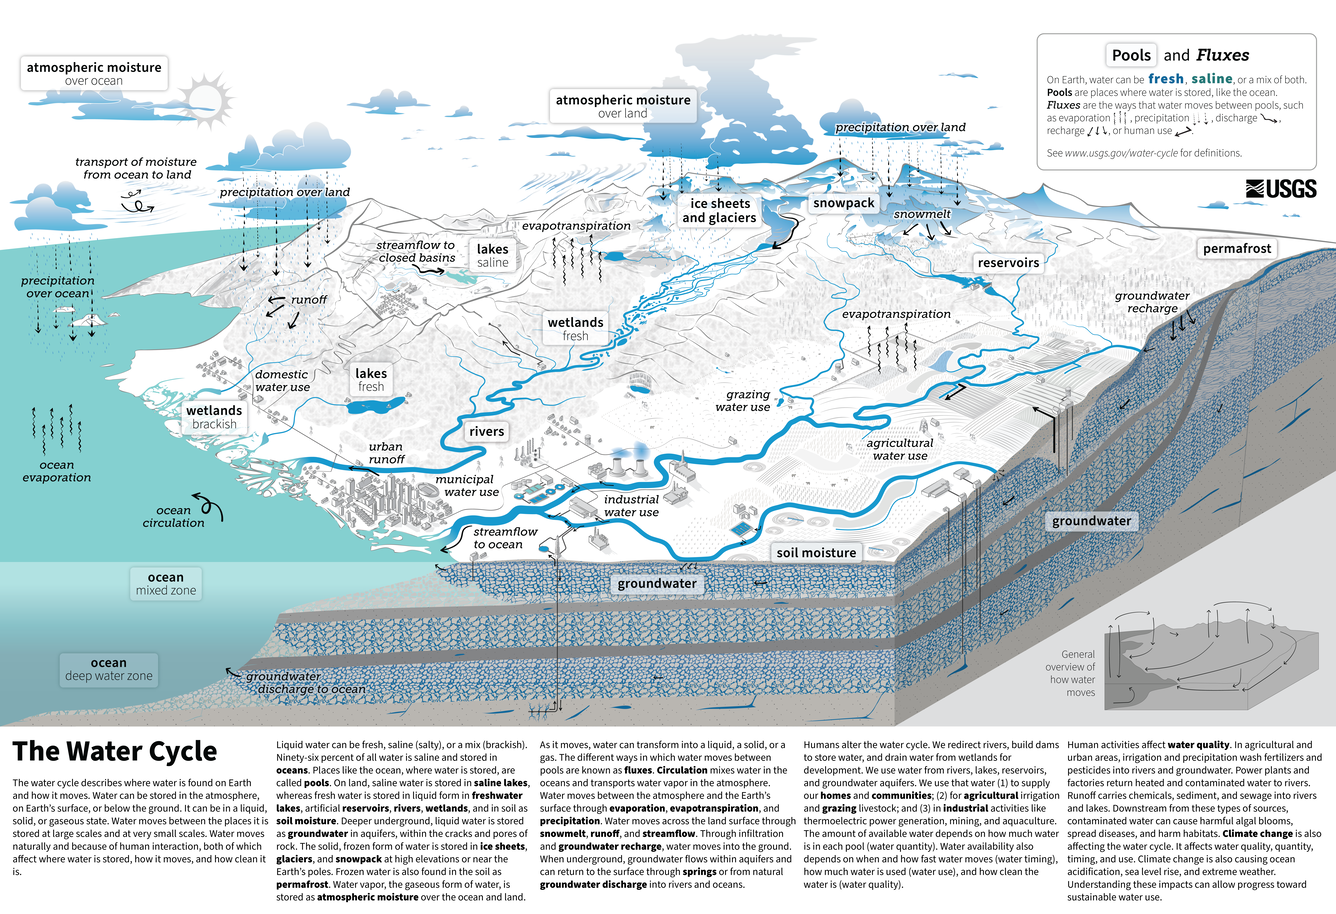
\includegraphics[keepaspectratio]{_assets/img/USGS_WaterCycle_English_ONLINE_20230302.png}}

}

\caption{The water cycle plays a key role in our climate system.
\href{https://labs.waterdata.usgs.gov/visualizations/water-cycle/index.html\#/}{\faIcon{camera-retro}:
USGS Water Cycle}}

\end{figure}%

\section{Statistical characteristics of climate
hazards}\label{statistical-characteristics-of-climate-hazards}

Climate hazards exhibit several key statistical properties that are
crucial for risk assessment and management. Understanding these
characteristics helps explain why traditional statistical approaches
often fail for climate extremes.

\subsection{Decision-theoretic
foundation}\label{decision-theoretic-foundation}

For any climate risk decision, we need to evaluate: \[
\mathbb{E}(R(a)) = \int_{\mathcal{S}} R(a, {\bf{s}}) p({\bf{s}}) d{\bf{s}}
\]

where \(a\) is a decision, \(R(a, {\bf{s}})\) is the reward/utility
function, and \({\bf{s}}\) represents the state of the climate system.

\textbf{Crucial insight}: \[
\mathbb{E}(R(a)) \neq R(a, \mathbb{E}({\bf{s}}))
\]

This means we cannot simply use ``average'' climate conditions to assess
risk. The full probability distribution \(p({\bf{s}})\) matters,
especially the tails.

\subsection{Key statistical
properties}\label{key-statistical-properties}

Climate hazards are characterized by:

\begin{itemize}
\tightlist
\item
  \textbf{Fat tails}: Extreme events are more probable than normal
  distributions predict
\item
  \textbf{Quasi-periodic oscillations}: Multi-year patterns like ENSO,
  AMO, PDO
\item
  \textbf{Non-stationarity}: Statistical properties change over time due
  to climate change
\item
  \textbf{Multi-scale variability}: Processes operate across temporal
  and spatial scales
\item
  \textbf{Spatial coherence}: Extreme events often affect large regions
  simultaneously
\item
  \textbf{Deep uncertainty}: Structural uncertainty about future climate
  evolution
\end{itemize}

\subsection{Examples of climate hazard
characteristics}\label{examples-of-climate-hazard-characteristics}

\subsubsection{Extreme events: recent
examples}\label{extreme-events-recent-examples}

\textbf{Floods in Paraguay, 2015}: Demonstrates the compound nature of
climate hazards, where prolonged precipitation combined with river basin
characteristics led to widespread inundation.

\textbf{Texas Cold Snap, 2021}: Illustrates how rare events outside the
historical range of variability can have catastrophic impacts on
unprepared infrastructure systems.

\subsubsection{Fat tails and extreme value
behavior}\label{fat-tails-and-extreme-value-behavior}

Many climate variables exhibit ``fat tail'' behavior, meaning extreme
values occur more frequently than predicted by normal distributions.
This has profound implications for: - Infrastructure design based on
return periods - Insurance and risk transfer mechanisms - Emergency
preparedness planning

\subsubsection{Non-stationarity and climate
change}\label{non-stationarity-and-climate-change}

Traditional statistical analysis assumes ``stationarity'' - that
statistical properties remain constant over time. Climate change
violates this assumption through: - Changing mean values (e.g., rising
temperatures) - Changing variability (e.g., intensifying precipitation
extremes) - Shifting seasonal patterns - Evolving spatial patterns of
extremes

\subsubsection{Multi-scale temporal
variability}\label{multi-scale-temporal-variability}

Climate hazards vary across multiple time scales: -
\textbf{Interannual}: El Niño-Southern Oscillation (2-7 years) -
\textbf{Decadal}: Atlantic Multidecadal Oscillation (60-80 years) -
\textbf{Centennial}: Long-term climate trends and solar cycles -
\textbf{Millennial}: Ice age cycles and geological forcing

This multi-scale nature means that short observational records may not
capture the full range of possible climate states.

\subsection{Implications for climate risk
assessment}\label{implications-for-climate-risk-assessment}

\subsubsection{Requirements for ``good'' climate
estimates}\label{requirements-for-good-climate-estimates}

To support decision-making, climate hazard characterizations should be:
- \textbf{Physically realistic}: Consistent with known climate processes
- \textbf{High resolution}: Adequate spatial and temporal detail for
impact assessment - \textbf{Uncertainty-aware}: Large ensemble sizes to
quantify uncertainty - \textbf{Scenario-inclusive}: Multiple plausible
futures for deep uncertainties

\subsubsection{Why extremes matter}\label{why-extremes-matter}

Climate risk assessment focuses on extremes because: - Most climate
impacts are driven by extreme events, not average conditions -
Infrastructure and ecosystems are often designed for historical extremes
- Climate change may disproportionately affect extreme events - Extreme
events drive most climate-related economic losses

\subsection{Discussion questions for climate
science}\label{discussion-questions-for-climate-science}

When studying climate science for risk assessment, consider these
questions:

\begin{itemize}
\tightlist
\item
  What are the challenges of using climate models to predict future
  climate?
\item
  What are the challenges of using climate models to predict future
  impacts?
\item
  How can observations help us understand future climate when the
  climate system is changing?
\item
  What is the difference between \textbf{climate risks} and
  \textbf{climate change risks}?
\item
  How should we plan for climate change impacts that are highly
  uncertain?
\end{itemize}

These questions highlight the intersection between physical climate
science and decision-making under uncertainty.

\section{What drives climate hazard
uncertainty?}\label{what-drives-climate-hazard-uncertainty}

Understanding the sources of uncertainty in climate hazard assessment is
crucial for effective risk management.

\subsection{Motivating applications}\label{motivating-applications}

\subsubsection{Stormwater infrastructure
design}\label{stormwater-infrastructure-design}

Consider sizing a stormwater pipe: 1. Use rainfall-runoff model:
\(Q = CiA\) (rational method) - \(i\) is rainfall intensity, \(A\) is
drainage area, \(C\) is runoff coefficient 2. Select design rainfall
based on return period \(T\): \(p(i > i^*) = 1/T\) 3. Size culvert to
handle design flow \(Q^* = Ci^*A\) 4. \textbf{Requires knowing} \(p(i)\)
- the probability distribution of rainfall intensity

\subsubsection{Floodplain mapping}\label{floodplain-mapping}

For riverine flood risk assessment: 1. Analyze historical streamflow
data at gauge locations 2. Estimate the 99th percentile (100-year return
level) of annual maximum flows 3. Use hydraulic models to map flood
extent and depths 4. \textbf{Requires understanding} the probability
distribution of extreme flows

\subsubsection{Reservoir design and
operations}\label{reservoir-design-and-operations}

For water supply reliability: 1. Consider \(N\) years of inflows,
releases, and evaporation 2. Count failure events (reservoir emptying)
3. Repeat with different flow scenarios 4. \textbf{If sampling from}
\(p(\text{inflow})\), estimate system reliability using Monte Carlo
methods

\subsubsection{Index insurance pricing}\label{index-insurance-pricing}

For weather-based insurance products: 1. Define insurance index \(I\)
(e.g., total seasonal rainfall) 2. Set threshold \(I^*\) for payouts of
amount \(X\) 3. Payout probability: \(p^* = p(I > I^*)\) 4. Risk
premium:
\(R = X \left( \mathbb{E}[p^*] + \lambda \mathbb{V}^{1/2}[p^*] \right)\)
5. \textbf{Requires estimating} probability distributions and their
uncertainty

\subsection{Case study: storm surge risk
assessment}\label{case-study-storm-surge-risk-assessment}

\subsubsection{Problem statement}\label{problem-statement}

Design a storm surge barrier for Galveston Bay. What is the probability
distribution of storm surge at your location?

This requires understanding multiple components:

\subsubsection{Historical data analysis}\label{historical-data-analysis}

\begin{itemize}
\tightlist
\item
  \textbf{Advantages}: Measures actual hazards at locations of interest
\item
  \textbf{Limitations}:

  \begin{itemize}
  \tightlist
  \item
    Sampling uncertainty from short records
  \item
    Doesn't account for changing future conditions
  \item
    Limited spatial coverage
  \end{itemize}
\end{itemize}

\subsubsection{Tropical cyclone
characteristics}\label{tropical-cyclone-characteristics}

To generate synthetic storm records, we need to model: - Storm tracks
and intensities - Wind and precipitation fields - Storm surge physics
using models (ADCIRC, GeoClaw, SFINCS)

\subsubsection{Sea level rise scenarios}\label{sea-level-rise-scenarios}

Future storm surge risk depends on: 1. Greenhouse gas emissions
scenarios 2. Climate system sensitivity to CO₂ 3. Ice sheet response to
warming 4. Local land subsidence rates

\subsubsection{Model limitations and
uncertainties}\label{model-limitations-and-uncertainties}

Recent research highlights persistent model biases: \textgreater{}
``Models are incorrectly simulating the equatorial Pacific response to
greenhouse gas warming. This implies that projections of regional
tropical cyclone activity may be incorrect as well'' (Sobel et al. 2023)

\subsection{Sources of uncertainty}\label{sources-of-uncertainty}

\subsubsection{Historical Data}\label{historical-data}

\begin{itemize}
\tightlist
\item
  \textbf{Strengths}: Direct measurement of hazards
\item
  \textbf{Weaknesses}: Sampling uncertainty, limited to past conditions
\end{itemize}

\subsubsection{Model Simulations}\label{model-simulations}

\begin{itemize}
\tightlist
\item
  \textbf{Strengths}: Can explore future scenarios, larger sample sizes
\item
  \textbf{Weaknesses}: Model structure uncertainty, potential biases
\end{itemize}

\subsubsection{Deep Uncertainty}\label{deep-uncertainty}

Many aspects of future climate involve ``deep uncertainty'': - Unknown
probability distributions - Uncertain model structure - Ambiguous
scenario definitions

\subsection{Key concepts and
terminology}\label{key-concepts-and-terminology}

\begin{itemize}
\tightlist
\item
  \textbf{Return Period}: Average time between exceedances of a
  threshold
\item
  \textbf{Return Level}: Magnitude of event associated with a given
  return period\\
\item
  \textbf{Monte Carlo}: Statistical sampling method for uncertainty
  quantification
\item
  \textbf{Synthetic Record}: Model-generated data extending historical
  observations
\item
  \textbf{Climate Sensitivity}: Global temperature response to CO₂
  doubling
\end{itemize}

\section{Earth's energy balance and greenhouse
effect}\label{earths-energy-balance-and-greenhouse-effect}

\emph{{[}This section to be developed with fundamental climate
physics{]}}

\section{Multi-scale variability}\label{multi-scale-variability}

\emph{{[}This section to be developed with climate system dynamics{]}}

\section{Basics of GCMs and Earth system
models}\label{basics-of-gcms-and-earth-system-models}

\emph{{[}This section to be developed with climate model
fundamentals{]}}

\section*{Further reading}\label{further-reading-1}
\addcontentsline{toc}{section}{Further reading}

\markright{Further reading}

\chapter{Probability and Inference ✏️}\label{probability-and-inference}

\section*{Learning objectives}\label{learning-objectives-1}
\addcontentsline{toc}{section}{Learning objectives}

\markright{Learning objectives}

After reading this chapter, you should be able to:

\begin{itemize}
\tightlist
\item
  Understand foundational probability concepts (random variables,
  distributions, moments).
\item
  Apply descriptive and inferential statistical methods to
  climate-related datasets.
\item
  Recognize when and why certain probability models are appropriate for
  climate variables.
\end{itemize}

\section{Three steps of probabilistic
inference}\label{three-steps-of-probabilistic-inference}

Before diving into the mathematical foundations, let's establish what
we're trying to accomplish with probabilistic methods in climate risk
assessment. \textbf{Probabilistic inference} is fundamentally about
learning from data to make decisions under uncertainty.

Following Gelman et al. (2014), we can organize all of probabilistic
modeling into three essential steps:

\begin{enumerate}
\def\labelenumi{\arabic{enumi}.}
\tightlist
\item
  \textbf{Set up a full probability model}: Define a joint probability
  distribution for all observable and unobservable quantities in your
  problem
\item
  \textbf{Condition on observed data}: Calculate the posterior
  distribution of unknown quantities given what you've observed
\item
  \textbf{Evaluate the fit and implications}: Check how well the model
  captures reality and what it implies for decisions
\end{enumerate}

This three-step workflow applies whether you're estimating flood return
periods, projecting future hurricane intensities, or evaluating
adaptation strategies. Let's see this in action with a simple example
before diving into the mathematical machinery.

\subsection{A simple example: Coin
flipping}\label{a-simple-example-coin-flipping}

Let's start with the simplest possible example to illustrate the
three-step workflow. Suppose you have a coin and want to know if it's
fair. This simple model is analogous to many real-world risk problems:
for example, asking if a given year has a `high' or `low' chance of
experiencing a major flood based on a complex climate model's binary
prediction. In both cases, we have a binary outcome and want to infer
the underlying probability.

\textbf{Step 1 - Set up the model}: - Parameter of interest: \(\theta\)
= probability the coin lands heads - Prior belief: maybe the coin is
fair, so \(\theta\) could be around 0.5 - Data model: each flip follows
\(\text{Bernoulli}(\theta)\)

\textbf{Step 2 - Learn from data}: You flip the coin 10 times and
observe 7 heads. Use Bayes' theorem to update your belief about
\(\theta\).

\textbf{Step 3 - Make decisions}: Based on your posterior distribution
for \(\theta\), decide whether the coin is likely fair or biased.

This simple example captures the essence of probabilistic inference.
We'll formalize this logic throughout the chapter, then apply it to much
more complex climate risk problems.

\section{The language of uncertainty}\label{the-language-of-uncertainty}

We assume you have taken courses in probability and statistics and are
familiar with basic concepts. This section provides a focused review of
essential foundations, emphasizing how they serve probabilistic
inference for climate risk. For more mathematical details,
\href{https://betanalpha.github.io/writing/}{Michael Betancourt's
writing} is an outstanding resource.

\subsection{General notation for statistical
inference}\label{general-notation-for-statistical-inference}

Before developing the theory, let's establish clear notation that we'll
use throughout the book. Following Gelman et al. (2014), we distinguish
three types of quantities:

\begin{itemize}
\tightlist
\item
  \textbf{Parameters} (\(\theta\)): Unknown quantities we want to learn
  about (e.g., the true 100-year flood level, hurricane intensity
  parameters, or climate sensitivity)
\item
  \textbf{Observed data} (\(y\)): Quantities we have measured (e.g.,
  historical flood heights, satellite temperature measurements, or storm
  track records)
\item
  \textbf{Unobserved predictions} (\(\tilde{y}\)): Unknown but
  potentially observable quantities (e.g., next year's maximum
  temperature, future sea level, or the outcome of a proposed adaptation
  strategy)
\end{itemize}

The \textbf{joint probability model} \(p(\theta, y, \tilde{y})\)
describes our beliefs about all these quantities and their
relationships. This joint distribution is the central object in
probabilistic inference---everything else flows from asking questions of
this distribution.

For climate risk assessment, \(\theta\) might represent physical
parameters like climate sensitivity or return period parameters, \(y\)
represents our historical observations and measurements, and
\(\tilde{y}\) represents future climate conditions we need to predict
for planning.

\subsection{Exchangeability}\label{exchangeability}

A fundamental assumption underlying most statistical models is
\textbf{exchangeability}: the idea that we can learn about future
observations from past observations because they share some common
underlying structure.

Two random variables \(Y_1\) and \(Y_2\) are exchangeable if their joint
distribution is unchanged by swapping their labels:
\(p(Y_1, Y_2) = p(Y_2, Y_1)\). More generally, observations
\(Y_1, \ldots, Y_n\) are exchangeable if their joint distribution is
invariant under permutations.

For climate applications, exchangeability justifies using historical
flood records to estimate future flood risk, or using temperature
measurements from different years to understand temperature variability.
However, exchangeability can break down when the underlying system
changes---for instance, due to climate change or urbanization affecting
flood patterns.

\subsection{Axiomatic foundations}\label{axiomatic-foundations}

Probability theory rests on three simple axioms that ensure
probabilities behave consistently: they're non-negative, total
probability equals one, and probabilities of mutually exclusive events
add up. From these basic rules, we can derive all the mathematical
machinery needed for probabilistic inference (Jaynes 2003).

\subsection{Joint distributions}\label{joint-distributions}

The central concept in probabilistic inference is the \textbf{joint
probability distribution}. For any problem involving uncertainty, our
goal is to specify a joint distribution over all relevant
quantities---both observed and unobserved.

The joint distribution \(p(\theta, y, \tilde{y})\) completely
characterizes our knowledge state about:

\begin{itemize}
\tightlist
\item
  What we want to learn (parameters \(\theta\))
\item
  What we have observed (data \(y\))\\
\item
  What we want to predict (future observations \(\tilde{y}\))
\end{itemize}

Everything else in probabilistic inference involves asking questions of
this joint distribution:

\begin{itemize}
\tightlist
\item
  \textbf{Learning from data}: \(p(\theta | y) \propto p(\theta, y)\)
  (conditioning)
\item
  \textbf{Making predictions}:
  \(p(\tilde{y} | y) = \int p(\tilde{y}, \theta | y) d\theta\)
  (marginalization)
\item
  \textbf{Quantifying decision-relevant quantities}:
  \(\mathbb{E}[f(\theta, \tilde{y}) | y]\) (expectation of functions)
\end{itemize}

This perspective---that statistical modeling is about building joint
distributions---provides the foundation for the computational methods
we'll develop later.

\subsection{Bayes' theorem}\label{bayes-theorem}

\textbf{Bayes' theorem} connects the different types of probability
statements and provides the foundation for updating beliefs based on
evidence. Since joint probability can be decomposed as
\(p(\theta, y) = p(\theta) p(y | \theta) = p(y) p(\theta | y)\), we can
derive:

\[
p(\theta | y) = \frac{p(\theta) p(y | \theta)}{p(y)}
\]

This equation has a powerful interpretation: \(p(\theta)\) represents
our \textbf{prior} beliefs about parameters \(\theta\),
\(p(y | \theta)\) represents the \textbf{likelihood} of observing data
\(y\) given parameters \(\theta\), and \(p(\theta | y)\) represents our
\textbf{posterior} beliefs after seeing the data.

In many applications, we work with the \textbf{proportional form}
\(p(\theta | y) \propto p(\theta) p(y | \theta)\) since the denominator
\(p(y)\) doesn't depend on \(\theta\). This framework is essential for
\textbf{Bayesian inference} in climate science, where we often want to
update our understanding of physical processes based on observations.

\section{Using probability models to learn from
data}\label{using-probability-models-to-learn-from-data}

\textbf{Probability theory} gives us the language for representing
uncertainty, but \textbf{probabilistic inference} is about using that
language to answer specific questions. Given a joint probability model
\(p(\theta, y, \tilde{y})\), we need computational tools to extract the
information relevant for decision-making.

All probabilistic inference involves two fundamental operations on the
joint distribution:

\subsection{The two fundamental
operations}\label{the-two-fundamental-operations}

\subsubsection{1. Conditioning: Learning from
data}\label{conditioning-learning-from-data}

\textbf{Conditioning} answers: ``How does observing data \(y\) change
our beliefs about parameters \(\theta\)?''

We use \textbf{Bayes' theorem} to compute the posterior distribution:
\[p(\theta | y) = \frac{p(\theta, y)}{p(y)} = \frac{p(\theta) p(y | \theta)}{\int p(\theta) p(y | \theta) d\theta}\]

The posterior \(p(\theta | y)\) represents our updated knowledge about
\(\theta\) after seeing data \(y\). This is the mathematical engine for
learning---it tells us how to rationally update our beliefs based on
evidence.

For climate risk assessment, conditioning might update our beliefs
about:

\begin{itemize}
\tightlist
\item
  Hurricane intensity parameters after observing a new storm season
\item
  Flood return levels after observing recent extreme events\\
\item
  Climate sensitivity parameters after incorporating new temperature
  data
\end{itemize}

\subsubsection{2. Marginalization: Focusing on what
matters}\label{marginalization-focusing-on-what-matters}

\textbf{Marginalization} answers: ``What do we know about quantity
\(\theta_1\) while ignoring nuisance parameters \(\theta_2\)?''

We integrate out unwanted variables to focus on quantities of interest:
\[p(\theta_1 | y) = \int p(\theta_1, \theta_2 | y) d\theta_2\]

This allows us to extract the uncertainty in specific parameters while
averaging over everything else we don't care about for a particular
decision.

For example, when estimating flood risk, we might marginalize over
uncertain rainfall distribution parameters to focus solely on the flood
frequency we need for infrastructure planning.

\subsection{Computing expectations}\label{computing-expectations}

These two operations ultimately serve one purpose: computing
\textbf{expectations} that inform decisions. When we need to know the
probability of an event or the expected value of some quantity of
interest, we often need to apply both conditioning and marginalization
to extract that information from our joint distribution.

The goal of probabilistic inference is computing \textbf{expectations}
--- probability-weighted averages of quantities we care about. Most
decision-relevant quantities can be expressed as an expectation:

\begin{itemize}
\tightlist
\item
  The \textbf{mean} is \(\mathbb{E}[X]\)
\item
  The \textbf{variance} is \(\mathbb{E}[(X - \mathbb{E}[X])^2]\)
\item
  The \textbf{probability of an event} is
  \(\mathbb{E}[\mathbf{1}_{\text{event}}]\) (expectation of an indicator
  function)
\item
  \textbf{Expected annual damages} from hurricanes integrate over storm
  intensity, frequency, and damage functions
\item
  \textbf{Failure probabilities} for infrastructure under extreme heat
  integrate over temperature distributions and failure thresholds
\end{itemize}

Formally, we want to compute:
\[\mathbb{E}[g(\theta, \tilde{y}) | y] = \int g(\theta, \tilde{y}) p(\theta, \tilde{y} | y) d\theta d\tilde{y}\]

where \(g(\theta, \tilde{y})\) is some function of our parameters and
predictions that captures what we need for decision-making.

\subsubsection{Analytical vs computational
approaches}\label{analytical-vs-computational-approaches}

For simple models, we can sometimes compute expectations analytically by
solving integrals directly. But for the complex, high-dimensional
problems typical in climate risk assessment, we need computational
approaches:

\textbf{Monte Carlo estimation} approximates expectations by: 1. Drawing
many samples from the probability model:
\((\theta^{(1)}, \tilde{y}^{(1)}), \ldots, (\theta^{(S)}, \tilde{y}^{(S)})\)
2. Computing the function of interest:
\(g(\theta^{(s)}, \tilde{y}^{(s)})\) for each sample 3. Averaging:
\(\mathbb{E}[g(\theta, \tilde{y}) | y] \approx \frac{1}{S} \sum_{s=1}^S g(\theta^{(s)}, \tilde{y}^{(s)})\)

This approach forms the foundation for computational methods we'll
develop in subsequent chapters.

\subsection{Interpreting probability}\label{interpreting-probability}

Now that we've seen how expectations drive decision-making, it's worth
reflecting on what the probabilities in these expectations \emph{mean}.
This philosophical question becomes crucial when studying extreme events
and catastrophic risks that cannot be objectively verified through
repeated experimentation.

\textbf{Frequentist (objective) interpretation} views probability as
limiting frequencies of repeatable events. Under this view, statements
like ``the probability of a category 5 hurricane is 0.02'' refer to
long-run frequencies we could observe if we repeated the same conditions
many times.

\textbf{Bayesian (subjective/epistemic) interpretation} views
probability as degrees of belief or states of knowledge. Here,
probability statements reflect our uncertainty given available
information, even for unique events like ``the probability that sea
level rise exceeds 1 meter by 2100.''

For extreme events and catastrophic risks, the Bayesian interpretation
is often more useful because:

\begin{itemize}
\tightlist
\item
  Many catastrophic events are rare or unique (we can't repeat the
  experiment)
\item
  We often need to reason about future scenarios that have never
  occurred
\item
  Scientific knowledge combines multiple sources of uncertain
  information
\end{itemize}

\subsection{Computational approaches}\label{computational-approaches}

The Bayesian framework naturally leads us to computational methods for
calculating expectations, since the required integrals are often
intractable analytically.

\subsubsection{Law of large numbers}\label{law-of-large-numbers}

The \textbf{law of large numbers} justifies this approach by formalizing
that sample averages converge to true expectations. For independent,
identically distributed random variables \(X_1, X_2, \ldots\) with mean
\(\mu\): \[
\lim_{n \to \infty} \frac{1}{n} \sum_{i=1}^n X_i = \mu
\]

For catastrophic risk assessment, this means:

\begin{itemize}
\tightlist
\item
  Monte Carlo estimates of expected annual losses become more accurate
  with more simulations
\item
  Historical averages of rare event frequencies converge to true rates
  (given stationarity)
\item
  Complex expectations over joint distributions of multiple hazards can
  be reliably estimated
\end{itemize}

However, for extreme events, convergence can be \textbf{slow} due to
heavy tails and rare events. Estimating expectations of catastrophic
losses may require many thousands of simulations to achieve reasonable
accuracy.

\subsubsection{Central limit theorem}\label{central-limit-theorem}

The law of large numbers tells us that Monte Carlo estimates converge,
but how uncertain are our estimates? The \textbf{central limit theorem}
quantifies this uncertainty: our sample average \(\bar{Y}\) is
approximately normally distributed around the true expectation \(\mu\):

\[\bar{Y} \sim \mathcal{N}\left(\mu, \frac{\sigma^2}{n}\right)\]

For catastrophic risk assessment, this means we can quantify the
\textbf{Monte Carlo uncertainty} in our estimates of expected annual
losses, failure probabilities, and other risk metrics. This is crucial
for decision-making because it distinguishes between uncertainty in our
estimates (which decreases with more simulation) and fundamental
uncertainty about the underlying extreme event processes.

Statistical inference for extreme events involves making conclusions
about catastrophic risks from limited data. Two fundamentally different
philosophical approaches dominate, each with important implications for
how we understand and communicate about rare event risks.

\subsubsection{Frequentist vs Bayesian
approaches}\label{frequentist-vs-bayesian-approaches}

\textbf{Frequentist inference} treats the parameters of extreme event
distributions (like hurricane intensity parameters or flood return
levels) as fixed but unknown quantities. Under this approach,
uncertainty comes from sampling variability---we'd get different
parameter estimates if we observed different historical samples.
Confidence intervals represent the variability we'd expect across many
hypothetical repetitions of the same data collection process.

\textbf{Bayesian inference} treats parameters as random variables
representing our knowledge state. Prior distributions encode our beliefs
about plausible parameter values (perhaps from physical understanding or
regional climate information), which get updated with observed data to
produce posterior distributions representing our updated knowledge.

For catastrophic risk assessment, the philosophical difference matters:

\begin{itemize}
\tightlist
\item
  Frequentist: ``Given these fixed (unknown) hurricane parameters,
  there's a 5\% chance our confidence interval won't contain the true
  100-year return level''
\item
  Bayesian: ``Given our data and prior knowledge, there's a 95\%
  probability the 100-year return level lies in this credible interval''
\end{itemize}

\subsubsection{Why Bayesian methods suit extreme
events}\label{why-bayesian-methods-suit-extreme-events}

Bayesian approaches prove particularly valuable for extreme event
analysis because:

\begin{itemize}
\tightlist
\item
  \textbf{Limited data}: Extreme events are rare, making prior knowledge
  from physical processes crucial
\item
  \textbf{Decision focus}: Decisions require acting on current
  knowledge, not hypothetical repetitions
\item
  \textbf{Unique events}: Many catastrophic scenarios (like worst-case
  sea level rise) are inherently unique
\item
  \textbf{Uncertainty propagation}: Complex models benefit from full
  uncertainty characterization
\end{itemize}

\subsubsection{Hypothesis testing for
extremes}\label{hypothesis-testing-for-extremes}

A common practical question is whether observed data are consistent with
specific hypotheses about extreme event behavior---for instance, testing
whether hurricane intensities show trends or whether flood frequencies
have changed. Both frequentist and Bayesian frameworks provide tools for
these questions, though they interpret the results differently.

\section{Probability building blocks}\label{probability-building-blocks}

The inference framework above relies on several key probability
concepts. This section provides the essential building blocks for
constructing probability models.

\subsection{Random variables}\label{random-variables}

A \textbf{random variable} is a function that assigns numerical values
to outcomes of random experiments. We use capital letters (\(X\), \(Y\),
\(Z\)) to denote random variables and lowercase letters (\(x\), \(y\),
\(z\)) for their specific realizations or values.

For catastrophic risk applications, \(X\) might represent ``maximum
storm surge height during a hurricane'' and \(x = 4.2\) meters would be
a specific observation. \textbf{Continuous random variables} (like storm
surge heights, wildfire burned area, or drought duration) can take any
value in an interval, while \textbf{discrete random variables} (like the
annual number of Category 4+ hurricanes or power outage events) take
countable values.

\subsection{CDFs, PDFs, and PMFs}\label{cdfs-pdfs-and-pmfs}

To work with random variables, we need functions that describe how
probability is distributed across possible values.

The \textbf{cumulative distribution function (CDF)} answers ``what is
the probability that \(X\) is at most \(x\)?'':
\[F_X(x) = \Pr(X \leq x)\]

For continuous random variables, we work with \textbf{probability
density functions (PDFs)}. The density \(f_X(x)\) represents probability
per unit length, related to the CDF through calculus:
\[F_X(x) = \int_{-\infty}^x f_X(u) \, du \quad \text{and} \quad f_X(x) = \frac{d}{dx}F_X(x)\]

We calculate probabilities by integrating the PDF over intervals:
\[\Pr[a \leq X \leq b] = \int_a^b f_X(x) \, dx\]

\begin{tcolorbox}[enhanced jigsaw, arc=.35mm, breakable, title=\textcolor{quarto-callout-important-color}{\faExclamation}\hspace{0.5em}{Important}, coltitle=black, opacityback=0, bottomtitle=1mm, colback=white, left=2mm, opacitybacktitle=0.6, toptitle=1mm, colframe=quarto-callout-important-color-frame, leftrule=.75mm, titlerule=0mm, rightrule=.15mm, bottomrule=.15mm, colbacktitle=quarto-callout-important-color!10!white, toprule=.15mm]

For continuous random variables, \(\Pr(X = x^*) = 0\) for any specific
value \(x^*\). Probability is concentrated over intervals, not points.

\end{tcolorbox}

\textbf{Discrete random variables} use \textbf{probability mass
functions (PMFs)} instead: \(p_X(x) = \Pr(X = x)\). Unlike continuous
variables, discrete variables can assign non-zero probability to
individual values.

\subsection{Marginal, conditional, and joint
distributions}\label{marginal-conditional-and-joint-distributions}

Catastrophic events often involve multiple interacting hazards---storm
surge and wind speed during hurricanes, temperature and drought severity
during heat waves, or rainfall intensity and duration during floods.
Understanding these \textbf{compound extremes} requires working with
multiple random variables simultaneously.

\textbf{Joint probability} describes multiple extreme events occurring
together: \(p(x, y)\) for joint densities or \(\Pr(X = x, Y = y)\) for
discrete events. This answers questions like ``what's the probability of
both extreme storm surge AND category 4+ winds?'' --- critical for
compound hurricane risk.

\textbf{Marginal probability} focuses on one hazard while ignoring
others: \(p(x)\) for continuous variables or \(\Pr(X = x)\) for discrete
events. For instance, the marginal distribution of wildfire burned area
ignores weather conditions, even though they strongly influence fire
behavior.

\textbf{Conditional probability} describes one extreme given another has
occurred: \(p(x | y)\) for conditional densities or
\(\Pr(X = x | Y = y) = \frac{\Pr(X = x, Y = y)}{\Pr(Y = y)}\) for
discrete events. This answers questions like ``given an extreme heat
event, what's the distribution of drought severity?'' --- essential for
cascading risk assessment.

\subsection{Independence}\label{independence}

Two events \(A\) and \(B\) are \textbf{independent} if knowing that one
occurred provides no information about the other. Mathematically,
independence means: \[\Pr(A \cap B) = \Pr(A) \cdot \Pr(B)\]

Equivalently, for independent events: \(\Pr(A | B) = \Pr(A)\) and
\(\Pr(B | A) = \Pr(B)\).

For random variables \(X\) and \(Y\), independence means the joint
density factorizes: \(p(x, y) = p(x) \cdot p(y)\). This is a strong
assumption that often doesn't hold in climate systems---temperature and
precipitation are typically dependent, as are wind speed and atmospheric
pressure.

\textbf{Conditional independence} is also important: \(X\) and \(Y\) may
be dependent overall but independent given knowledge of a third variable
\(Z\). This concept is crucial for understanding how climate variables
relate through mediating factors.

\subsection{Common probability
distributions}\label{common-probability-distributions}

Several key distributions appear frequently in catastrophe modeling and
extreme event analysis:

\begin{itemize}
\tightlist
\item
  The \textbf{Poisson distribution} \(Y \sim \text{Poisson}(\lambda)\)
  models rare event counts like annual numbers of Category 4+
  hurricanes, major earthquakes, or wildfire ignitions over fixed
  periods.
\item
  The \textbf{Negative Binomial distribution} handles overdispersed
  extreme event counts when variance exceeds the mean---common when
  events cluster in time (like hurricane seasons).
\item
  The \textbf{Gamma distribution} models positive-valued extremes like
  maximum daily rainfall amounts, drought durations, and time between
  major flood events.
\item
  The \textbf{Weibull distribution} is fundamental for extreme value
  analysis, modeling phenomena like maximum wind speeds, peak storm
  surge heights, and infrastructure failure times.
\item
  \textbf{Generalized Extreme Value (GEV)} and \textbf{Generalized
  Pareto (GP)} distributions specifically model the statistical behavior
  of extreme values and exceedances over high thresholds---foundational
  for catastrophe risk assessment.
\end{itemize}

\subsubsection{Moments}\label{moments}

The \textbf{moments} of a distribution characterize its shape and
properties---particularly important for understanding extreme event
behavior. The first few moments have direct interpretations for
catastrophe modeling:

\begin{itemize}
\tightlist
\item
  \textbf{First moment (mean)}: \(\mathbb{E}[X] = \mu\) - the center of
  the distribution
\item
  \textbf{Second central moment (variance)}:
  \(\text{Var}(X) = \mathbb{E}[(X - \mu)^2] = \sigma^2\) - spread around
  the mean\\
\item
  \textbf{Third central moment (skewness)}: measures asymmetry -
  positive skew indicates long right tails with rare extreme values
\item
  \textbf{Fourth central moment (kurtosis)}: measures tail heaviness -
  higher kurtosis means more frequent extreme values
\end{itemize}

For catastrophic events, \textbf{skewness} and \textbf{kurtosis} are
crucial. Storm surge heights typically show positive skew (most events
are small, rare events are catastrophic), while wildfire burned areas
often exhibit heavy tails with extreme kurtosis during exceptional fire
seasons.

\section*{Further reading}\label{further-reading-2}
\addcontentsline{toc}{section}{Further reading}

\markright{Further reading}

If most of this content is unfamiliar to you, reviewing a more
comprehensive introduction to probability and statistics before
proceeding may be helpful. While introductory statistics is often taught
in a dry way, Blitzstein and Hwang (2019), Downey (2021), and Gelman
(2021) are three excellent resources that I highly recommend (see
\href{./chapters/about/resources.qmd}{recommended reading} for more
suggestions).

\chapter{Optimization ✏️}\label{optimization}

\section*{See first}\label{see-first}
\addcontentsline{toc}{section}{See first}

\markright{See first}

This chapter builds on concepts from: -
\href{./chapters/fundamentals/probability-stats.qmd}{Probability and
Statistics}

\section*{Learning objectives}\label{learning-objectives-2}
\addcontentsline{toc}{section}{Learning objectives}

\markright{Learning objectives}

\begin{itemize}
\tightlist
\item
  Understand the components of an optimization problem: decision
  variables, objective functions, and constraints.
\item
  Learn how optimization is applied in statistics and policy search.
\item
  Explore the trade-offs between problem complexity and solution
  accuracy.
\end{itemize}

Optimization is a field of study unto itself, and forms an essential
backbone of statistics, machine learning, and operations research. Here,
we briefly summarize key concepts and techniques in optimization, with a
focus on their application to statistics and policy search.

\section{Overview}\label{overview}

Optimization is the study of finding the best solution to a problem from
a set of feasible solutions. Thus, optimization problems typically
consist of

\begin{enumerate}
\def\labelenumi{\arabic{enumi}.}
\tightlist
\item
  A set of decision variables , \(x\), which are the inputs we can
  control (or the ``dials'' we can turn).
\item
  One (or more) objective function(s), \(f(x)\), which we want to
  minimize or maximize.
\item
  A set of constraints which define the feasible region.
\end{enumerate}

Optimization is an incredibly diverse field. Problems can have many
constraints or none; can have discrete or continuous decision variables
(or both); can be static or dynamic; deterministic or stochastic; linear
or nonlinear; or much more. When you encounter an optimization problem
in the wild, you should always make sure you understand the decision
variables (which define what is being optimized), the objective
function(s), which define what makes a solution ``good'', and the
constraints, which define what solutions are being considered. When you
build an optimization model, you should always make sure to communicate
these three components clearly.

Because optimization is a widely studied field, exact solutions to some
classes of problems are known, and nearly exact solutions to many others
are known. However, these exact solutions often require formulating the
problem in a very specific way. Thus, there is generally a trade-off
between designing an optimization problem that is (relatively) easy to
solve vs.~one that represents the relevant system dynamics and
uncertainties (relatively) accurately. Consequently, converting a
decision problem into an optimization problem is somewhat of an art
form, rather than an exact science; this is largely the field of
operations research.

\section{Motivation: Inference}\label{motivation-inference}

One common application of optimization is in statistics. Specifically,
we often want to evaluate how consistent the data are with different
values of the parameters, and to find the values of the parameters that
are most consistent with the data.

\subsection{General Case}\label{general-case}

\subsubsection{Likelihood}\label{likelihood}

The likelihood is the probability of the \textbf{observations} \(y\)
given some \textbf{parameters} \(\theta\): \[
p(y | \theta)
\]

Often, we want to study how the likelihood changes for different values
of \(\theta\), holding \(y\) fixed. This is just \(p(y | \theta)\) for a
range of \(\theta\).

\begin{tcolorbox}[enhanced jigsaw, arc=.35mm, breakable, title=\textcolor{quarto-callout-note-color}{\faInfo}\hspace{0.5em}{Note}, coltitle=black, opacityback=0, bottomtitle=1mm, colback=white, left=2mm, opacitybacktitle=0.6, toptitle=1mm, colframe=quarto-callout-note-color-frame, leftrule=.75mm, titlerule=0mm, rightrule=.15mm, bottomrule=.15mm, colbacktitle=quarto-callout-note-color!10!white, toprule=.15mm]

You will sometimes see this referred to as \(\mathcal{L}(\theta)\).
However, since this is a probability distribution, it doesn't really
need its own notation.

\end{tcolorbox}

\subsubsection{Likelihood function for multiple
observations}\label{likelihood-function-for-multiple-observations}

Often, we have multiple observations \(y_1, y_2, \ldots, y_n\).

Independent and identically distributed (i.i.d.) assumption: \[
\begin{aligned}
p(y_1, y_2, \ldots, y_n) &= p(y_1) p(y_2) \times \ldots \times p(y_n)\\
 &= \prod_{i=1}^n p(y_i)
\end{aligned}
\]

Usually we have more than one data point. Say we measure
\(y = y_1, y_2, \ldots, y_n\): \[
p(y | \theta) = \prod_{i=1}^n p(y_i | \theta)
\]

\subsubsection{Log trick}\label{log-trick}

Recall: \(\log(AB) = \log(A) + \log(B)\) or, more generally, \[
\log \left( \prod_{i=1}^n f_i \right) = \sum_{i=1}^n \log(f_i)
\]

Thus, we can work with the ``log likelihood'': \[
\log p(y | \theta) =  \log \left( \prod_{i=1}^n p(y_i | \theta) \right) = \sum_{i=1}^n \log \left( p(y_i | \theta) \right)
\]

Adding small numbers is also more numerically stable than multiplying
them

Can we find the parameters \(\theta^*\) that maximize the likelihood
\(p(y | \theta)\)?

\subsubsection{Log likelihood}\label{log-likelihood}

We can use the log likelihood \(\log p(y | \theta)\) instead of the
likelihood \(p(y | \theta)\).

The log likelihood is monotonic with the likelihood, so \[
\arg \max \log p(y | \theta) = \arg \max p(y | \theta)
\]

Solving things analytically takes time up-front, but can be much faster
to run because you can avoid the optimization step. Consider the
(potentially multivariate) Gaussian example with known covariance matrix
\(\Sigma\). We want to \emph{maximize} the likelihood \[
\sum_{i=1}^n p(y_i | \mu, \Sigma)
\]

To maximize, we set its derivative with respect to \(\mu\), which we'll
denote with \(\nabla_\mu\), to zero: \[
\sum_{i=1}^n \nabla_\mu \log p(y_i | \mu, \Sigma) = 0
\]

Substituting in the multivariate Gaussian likelihood we get: \[
\begin{aligned}
0 & =\sum_{i=1}^n \nabla_\mu \log \frac{1}{\sqrt{(2 \pi)^d|\Sigma|}} \exp \left(-\frac{1}{2}\left(x_i-\mu\right)^{\top} \Sigma^{-1}\left(x_i-\mu\right)\right) \\
& =\sum_{i=1}^n \nabla_\mu\left(\log \left(\frac{1}{\sqrt{(2 \pi)^d|\Sigma|}}\right)\right)+\log \left(\exp \left(-\frac{1}{2}\left(x_i-\mu\right)^{\top} \Sigma^{-1}\left(x_i-\mu\right)\right)\right) \\
& =\sum_{i=1}^n \nabla_\mu\left(-\frac{1}{2}\left(x_i-\mu\right)^{\top} \Sigma^{-1}\left(x_i-\mu\right)\right)\\
&=\sum_{i=1}^n \Sigma^{-1}\left(x_i-\mu\right) \\
0 &= \sum_{i=1}^n (x_i - \mu) \\
\mu &= \frac{1}{n} \sum_{i=1}^n x_i
\end{aligned}
\]

You are not expected to remember the above equations and I won't ask you
to do this derivation in a time-constrained exam. You should understand
the general procedure:

\begin{enumerate}
\def\labelenumi{\arabic{enumi}.}
\tightlist
\item
  write down log likelihood for all data points

  \begin{enumerate}
  \def\labelenumii{\arabic{enumii}.}
  \tightlist
  \item
    write down likelihood for one data point
  \item
    write down log likelihood for one data point
  \item
    sum over all data points
  \end{enumerate}
\item
  take \(\frac{d}{d\theta}\) and set equal to zero to maximize
\item
  solve for \(\theta^*\).
\end{enumerate}

\subsection{Example: Linear Regression}\label{example-linear-regression}

Let's consider the generic regression probelem where we have paired
observations \(\left\{x_i, y_i\right\}_{i=1}^n\). In general, we can
write this regression as \[
y_i | \alpha, \beta, \epsilon \sim \mathcal{N}(\alpha + x_i \beta, \sigma^2)
\] where \(x_i\) and \(\beta\) may be vectors.

We can use the same approach to derive the maximum likelihood estimate
for linear regression:

\begin{enumerate}
\def\labelenumi{\arabic{enumi}.}
\tightlist
\item
  Write the likelihood for one data point
\item
  Write the log likelihood for one data point
\item
  Write the log likelihood for all data points
\item
  Take \(\frac{d}{d\theta}\) and set equal to zero to maximize
\end{enumerate}

If you want a walkthrough, see
\href{https://www.cs.princeton.edu/courses/archive/fall18/cos324/files/mle-regression.pdf}{Ryan
Adams's lecture notes} starting at about equation 11.

If we work through the math, we can show that the log likelihood for the
linear regression problem is \[
\log p(y | X, \beta, \sigma) = \frac{N}{2} \log (2 \sigma^2 \pi)  - \frac{1}{2 \sigma^2} \left( X \beta - y \right)^T \left( X \beta - y \right)
\]

\begin{tcolorbox}[enhanced jigsaw, arc=.35mm, breakable, title=\textcolor{quarto-callout-note-color}{\faInfo}\hspace{0.5em}{Linear algebra notation}, coltitle=black, opacityback=0, bottomtitle=1mm, colback=white, left=2mm, opacitybacktitle=0.6, toptitle=1mm, colframe=quarto-callout-note-color-frame, leftrule=.75mm, titlerule=0mm, rightrule=.15mm, bottomrule=.15mm, colbacktitle=quarto-callout-note-color!10!white, toprule=.15mm]

There is no intercept here! This is a common notation and assumes that
the first column of \(X\) is all ones. That is equivalent to writing
down an intercept, but lets us use linear algebra notation and keep
track of fewer variable names

\end{tcolorbox}

From this, we can show that terms drop out and \[
\beta^\text{MLE} = \arg \min_\beta \left( X \beta - y \right)^T \left( X \beta - y \right)
\] which is exactly the least squares problem (minimize squared error):
\[
\min_{\theta} \sum_{i=1}^n (y_i - y_i^\text{pred})^2
\]

\begin{tcolorbox}[enhanced jigsaw, arc=.35mm, breakable, title=\textcolor{quarto-callout-important-color}{\faExclamation}\hspace{0.5em}{Key point}, coltitle=black, opacityback=0, bottomtitle=1mm, colback=white, left=2mm, opacitybacktitle=0.6, toptitle=1mm, colframe=quarto-callout-important-color-frame, leftrule=.75mm, titlerule=0mm, rightrule=.15mm, bottomrule=.15mm, colbacktitle=quarto-callout-important-color!10!white, toprule=.15mm]

``Least squares can be interpreted as assuming Gaussian noise, and
particular choices of likelihood can be interpreted directly as (usually
exponentiated) loss functions''
--\href{https://www.cs.princeton.edu/courses/archive/fall18/cos324/files/mle-regression.pdf}{Adams}

\end{tcolorbox}

If we then want to estimate \(\sigma\), we can estimate the standard
deviation of the residuals.

\begin{tcolorbox}[enhanced jigsaw, arc=.35mm, breakable, title=\textcolor{quarto-callout-tip-color}{\faLightbulb}\hspace{0.5em}{Computational examples}, coltitle=black, opacityback=0, bottomtitle=1mm, colback=white, left=2mm, opacitybacktitle=0.6, toptitle=1mm, colframe=quarto-callout-tip-color-frame, leftrule=.75mm, titlerule=0mm, rightrule=.15mm, bottomrule=.15mm, colbacktitle=quarto-callout-tip-color!10!white, toprule=.15mm]

For detailed computational examples of likelihood functions, MLE
estimation, and numerical optimization, see the companion file:
\href{./chapters/fundamentals/optimization-examples.qmd}{Maximum
Likelihood Estimation: Computational Examples}.

Examples include: - Plotting likelihood functions for single and
multiple data points - Poisson likelihood for count data (tropical
cyclone example)\\
- Multivariate likelihood surfaces - Numerical optimization with
\texttt{Optim.jl} - Linear regression MLE equivalence to least squares

\end{tcolorbox}

\section{Motivation: Policy Search}\label{motivation-policy-search}

\section{Optimization Toolkit}\label{optimization-toolkit}

\subsection{Gradient-Based
Optimization}\label{gradient-based-optimization}

This is useful for thinking about neural networks, but also for many
other optimization problems. The key idea is that we can use the
gradient of the objective function to find the direction in which to
move to improve our solution. This is often called \textbf{gradient
descent}. The basic idea is to take a step in the direction of the
gradient, which is the direction of steepest ascent. In the simplest
case, \[
\Delta x = -\alpha \nabla f(x)
\] where \(\alpha\) is the step size or learning rate. This is a
hyperparameter that we can tune.

The primary limitation of gradient descent is that it can get stuck in
local minima. This is especially true for non-convex problems, where
there may be many local minima. A vast range of techniques, a treatment
of which merits a textbook on its own, have been developed to address
this issue, including for example the Adam optimizer (Kingma and Ba
2017).

\subsection{Stochastic Optimization}\label{stochastic-optimization}

\subsection{Sequential Decision
Problems}\label{sequential-decision-problems}

\subsection{High-Dimensional
Optimization}\label{high-dimensional-optimization}

\section*{Further reading}\label{further-reading-3}
\addcontentsline{toc}{section}{Further reading}

\markright{Further reading}

\begin{itemize}
\tightlist
\item
  \textbf{Sutton and Barto (2018)} provides a comprehensive introduction
  to reinforcement learning, which is broadly the study of sequential
  decision-making under uncertainty.
\item
  \textbf{Powell (2022)} provides a comprehensive treatment of
  sequential decision-making under uncertainty, aiming at a unified
  framework
\end{itemize}

\chapter{Monte Carlo Methods ✏️}\label{monte-carlo-methods}

\section*{See first}\label{see-first-1}
\addcontentsline{toc}{section}{See first}

\markright{See first}

This chapter builds on concepts from: -
\href{./chapters/fundamentals/probability-stats.qmd}{Probability and
Statistics}

\section*{Learning objectives}\label{learning-objectives-3}
\addcontentsline{toc}{section}{Learning objectives}

\markright{Learning objectives}

\begin{itemize}
\tightlist
\item
  Apply Monte Carlo methods to approximate integrals and expectations
\item
  Use Markov Chain Monte Carlo (MCMC) techniques to estimate posterior
  distributions
\item
  Understand parameter uncertainty propagation in decision-making
\item
  Implement Monte Carlo simulation for climate risk assessment
\end{itemize}

Monte Carlo is a powerful class of methods used to estimate the
properties of a distribution by generating random samples from that
distribution. Specifically, Monte Carlo methods are used to estimate the
expected value of a function of random variables.

\section{Overview}\label{overview-1}

Monte Carlo methods are used to approximate integrals using sums. If we
want to compute an expectation \(\mathbb{E}[f(X)]\) where \(X\) has
probability density \(p(x)\):

\[
\mathbb{E}[f(X)] = \int f(x) p(x) dx
\]

we can approximate this using Monte Carlo: \[
\mathbb{E}[f(X)] \approx \frac{1}{N} \sum_{i=1}^N f(x_i)
\] where \(x_1, x_2, \ldots, x_N\) are samples drawn from \(p(x)\).

This is particularly powerful when \(p(x)\) is a complex posterior
distribution that we can only sample from, not evaluate directly.

\section{Motivation: Bayesian
inference}\label{motivation-bayesian-inference}

Bayesian inference provides a principled framework for updating our
beliefs about parameters given observed data. The key insight is that
parameters have probability distributions, not single point values.

\subsection{Bayes' theorem}\label{bayes-theorem-1}

For continuous parameters, Bayes' theorem states: \[
p(\theta | y) = \frac{p(y | \theta) p(\theta)}{p(y)}
\]

where: - \(p(\theta | y)\) is the \textbf{posterior} distribution (what
we want) - \(p(y | \theta)\) is the \textbf{likelihood} (probability of
data given parameters) - \(p(\theta)\) is the \textbf{prior}
distribution (our initial beliefs) - \(p(y)\) is the \textbf{marginal
likelihood} (normalizing constant)

Since \(p(y)\) doesn't depend on \(\theta\), we often work with: \[
p(\theta | y) \propto p(y | \theta) p(\theta)
\]

\subsection{The challenge}\label{the-challenge}

For most real-world problems, the posterior distribution
\(p(\theta | y)\) cannot be computed analytically. This is where Monte
Carlo methods become essential - we use them to draw samples from
complex posterior distributions.

\subsection{Markov Chain Monte Carlo
(MCMC)}\label{markov-chain-monte-carlo-mcmc}

MCMC methods generate samples from posterior distributions by: 1.
Starting at some initial parameter values 2. Proposing new parameter
values 3. Accepting or rejecting proposals based on the posterior
probability 4. Repeating to create a ``chain'' of samples

Modern MCMC algorithms like the No-U-Turn Sampler (NUTS) use gradient
information to efficiently explore high-dimensional parameter spaces.

\section{Motivation: parameter
uncertainty}\label{motivation-parameter-uncertainty}

A fundamental challenge in climate risk assessment is that model
parameters are uncertain. Consider a simple flood risk assessment
problem:

\begin{itemize}
\tightlist
\item
  We have a probability distribution for flood heights: \(p(h)\)
\item
  We have a damage function: \(d(h)\) (damages as a function of height)
\item
  We want the probability distribution of damages: \(p(d)\)
\end{itemize}

Mathematically: \[
p(d) = \int_h d(h) p(h) \, dh
\]

\subsection{The challenge}\label{the-challenge-1}

This integral is often impossible to solve analytically, especially
when: 1. We use realistic (non-analytical) damage functions 2. We want
to account for parameter uncertainty in \(p(h)\) 3. We have multiple
uncertain parameters

\subsection{Monte Carlo Solution}\label{monte-carlo-solution}

Instead of solving the integral analytically: 1. Sample flood heights:
\(h_1, h_2, \ldots, h_N \sim p(h)\) 2. Apply damage function:
\(d_i = d(h_i)\) for each sample 3. Analyze the resulting damage
samples: \(\{d_1, d_2, \ldots, d_N\}\)

This approach generalizes to complex, multi-parameter problems where
analytical solutions are impossible.

\section{Monte Carlo Theory}\label{monte-carlo-theory}

\subsection{Fundamental theorem}\label{fundamental-theorem}

If \(\theta^s \sim p(\theta)\), then by the Law of Large Numbers: \[
\mathbb{E}[f(\theta)] = \int_{\theta} f(\theta) p(\theta) d\theta \approx \frac{1}{S} \sum_{s=1}^S f(\theta^s)
\]

This convergence is \textbf{guaranteed} as \(S \to \infty\), making
Monte Carlo a robust approach for complex problems.

\subsection{Advantages over deterministic
integration}\label{advantages-over-deterministic-integration}

\textbf{Deterministic approach}: - Sample \(\theta\) at regular grid
points - Compute \(f(\theta)\) at each point and sum -
\textbf{Problems}: Curse of dimensionality, choice of grid spacing,
boundary handling

\textbf{Monte Carlo approach}: - Sample \(\theta\) from the actual
distribution \(p(\theta)\) - Automatically focuses computational effort
where probability is high - \textbf{Benefits}: Scales well to high
dimensions, handles complex domains

\section{Motivation: resilience}\label{motivation-resilience}

Monte Carlo methods are essential for resilience analysis because they
can handle: - Multiple uncertain hazards occurring simultaneously -
Complex system interactions and cascading failures - Non-linear damage
functions and thresholds - Rare but high-impact events

\section{Motivation: sensitivity
analysis}\label{motivation-sensitivity-analysis}

Monte Carlo methods excel at sensitivity analysis - understanding how
uncertain inputs affect outputs.

\subsection{Parameter sensitivity}\label{parameter-sensitivity}

By systematically varying parameters and observing changes in Monte
Carlo outputs, we can: 1. \textbf{Identify critical parameters}: Which
uncertainties matter most? 2. \textbf{Quantify sensitivity}: How much
does output uncertainty change with input uncertainty? 3. \textbf{Guide
data collection}: Where would additional measurements be most valuable?

\subsection{Global sensitivity
analysis}\label{global-sensitivity-analysis}

Unlike local sensitivity (derivatives at a point), Monte Carlo enables
\textbf{global sensitivity analysis} across the entire parameter space,
capturing: - Non-linear relationships - Parameter interactions -
Threshold effects - Tail behavior

\section{Bayesian Decision Theory
Context}\label{bayesian-decision-theory-context}

Recall from decision theory: \[
\mathbb{E}\left[L(a, \theta) \right] = \int_\theta L(a, \theta) p(\theta) d\theta
\] Where \(\theta\) is a vector of parameters, \(a\) is some action or
decision, and \(L\) is the loss function.

\begin{tcolorbox}[enhanced jigsaw, arc=.35mm, breakable, title=\textcolor{quarto-callout-note-color}{\faInfo}\hspace{0.5em}{Note}, coltitle=black, opacityback=0, bottomtitle=1mm, colback=white, left=2mm, opacitybacktitle=0.6, toptitle=1mm, colframe=quarto-callout-note-color-frame, leftrule=.75mm, titlerule=0mm, rightrule=.15mm, bottomrule=.15mm, colbacktitle=quarto-callout-note-color!10!white, toprule=.15mm]

We previously called \(\theta\) a ``state of the world'' and \(L\) a
``reward function''.

\end{tcolorbox}

\section{Practical problem: flood risk
assessment}\label{practical-problem-flood-risk-assessment}

You have been commissioned by a client to assess their exposure to
flooding. Specifically, they want to know the probability distribution
of annual flood damages at their property if they do not elevate or
floodproof their building.

\begin{enumerate}
\def\labelenumi{\arabic{enumi}.}
\tightlist
\item
  \(p(h)\): probability distribution of annual maximum flood heights at
  their property
\item
  \(d(h)\): flood damages as a deterministic function of flood height
\item
  \(p(d) = \int_h d(h) p(h) \, dh\)
\end{enumerate}

With this information, they can compute metrics like the expected annual
damage, the 99th percentile annual damage, and the probability of any
flood occurring that will help them make a decision.

\section{Functions of random variables: the
challenge}\label{functions-of-random-variables-the-challenge}

Plugging in a bounded logistic model for \(d(h)\) and our lognormal
model for \(h\): \[
\begin{align}
p(d) &= \int_h d(h) p(h) \, dh \\
&= \int_{-\infty}^\infty \mathbb{I}[h > 0] \text{logistic}(h) \mathcal{N}(h | \mu, \sigma^2) \, dh\\
&= \int_0^\infty \text{logistic}(h) \mathcal{N}(\mu, \sigma^2) \, dh\\
&= \int_0^\infty \frac{1}{1 + \exp(-k * (x - x0))} \frac {1}{\sigma {\sqrt {2\pi }}} \exp \left\{-{\frac {1}{2}}\left({\frac {x-\mu }{\sigma }}\right)^{2} \right\} \, dh
\end{align}
\]

\subsection{Limitations: analytic
approach}\label{limitations-analytic-approach}

We might be able to solve this analytically (Wolfram Alpha can't\ldots).
But:

\begin{enumerate}
\def\labelenumi{\arabic{enumi}.}
\tightlist
\item
  Numerous simplifying assumptions and approximations.
\item
  What if we want to use a different distribution?
\item
  A different damage model?
\end{enumerate}

\subsection{Monte Carlo Solution
Strategy}\label{monte-carlo-solution-strategy}

A deterministic strategy: 1. sample
\(h^s = 0, \Delta h, 2\Delta h, \ldots, (S-1)\Delta h\) 2. compute
\(\text{logistic}(h^s) \mathcal{N}(h^s | \mu, \sigma^2)\) at each point
and sum 3. drawbacks: we have to go to \(\infty\) and select
\(\Delta h\).

A sampling strategy: 1. sample \(h^1, h^2, \ldots, h^S \sim p(h)\) --
which we can do because we have a model for \(p(h)\) 2. for each value:
compute \(\mathbb{I}(h^s > 0) \text{logistic}(h^s)\) and take the
average 3. this converges to the correct expectation!

\section{Parameter uncertainty
propagation}\label{parameter-uncertainty-propagation}

\subsection{The core problem}\label{the-core-problem}

We have been working with a single probability distribution for flood
depths, which we computed by maximum likelihood.

These values are not precise. What happens if we consider the lognormal
distribution with slightly different, but still plausible, parameters?

What about the depth-damage parameters \(x_0\) and \(k\)?

\subsection{Parameter uncertainty
impact}\label{parameter-uncertainty-impact}

\begin{itemize}
\tightlist
\item
  Uncertainties in our model parameters propagate to uncertainties in
  the things we care about.
\item
  As we collect more data, fewer combinations of parameters are
  consistent with observations
\item
  Different parameter combinations can lead to substantially different
  risk assessments
\end{itemize}

\section{Bayesian Inference with
MCMC}\label{bayesian-inference-with-mcmc}

\subsection{Prior Information: A Simple
Example}\label{prior-information-a-simple-example}

Everyone is tested for CEVE543acitis, a rare and deadly disease: 1. It
is known that 1 in 1,000 people have CEVE543acitis 2. The test is 99\%
accurate 3. Your test comes back positive. What is the probability that
you have CEVE543acitis?

\subsection{Bayes' Rule: Discrete Event
Version}\label{bayes-rule-discrete-event-version}

\[
\Pr \left\{ \theta | y \right\} = \frac{\Pr \left\{ y | \theta \right\} \Pr \left\{ \theta \right\}}{\Pr \left\{ y \right\}}
\]

Define \(y\) is getting a positive test result and \(\theta\) is having
the underlying condition. Note that we do not observe \(\theta\)
directly! Here \(y=1\) and we want to know
\(\Pr\left\{\theta = 1 \mid y=1 \right\}\).

A naive application of maximum likelihood:
\(\Pr\left\{y=1 \mid \theta=1 \right\} > \Pr\left\{y=1 \mid \theta=0 \right\}\)
so best estimate is \(\theta=1\)

\subsection{Key Ideas for Bayesian
Inference}\label{key-ideas-for-bayesian-inference}

\begin{enumerate}
\def\labelenumi{\arabic{enumi}.}
\tightlist
\item
  Parameters have \textbf{probability distributions}, not single point
  values
\item
  Start with some prior distribution for parameters
\item
  Goal: what is the distribution of the parameters given the data?
\end{enumerate}

\subsection{Bayes' Rule for
Distributions}\label{bayes-rule-for-distributions}

\[
p(\theta \mid y) = \frac{p(y \mid \theta) p(\theta)}{p(y)}
\]

If we are drawing samples from a distribution, we can calculate up to a
constant of proportionality and -- since \(p(y)\) doesn't depend on
\(\theta\) -- we can usually ignore it.

\[
\overbrace{p(\theta \mid y)}^\rm{posterior} \propto \underbrace{p(y \mid \theta)}_\rm{likelihood} \overbrace{p(\theta)}^\rm{prior}
\]

\subsection{Markov Chain Monte Carlo
(MCMC)}\label{markov-chain-monte-carlo-mcmc-1}

\begin{enumerate}
\def\labelenumi{\arabic{enumi}.}
\tightlist
\item
  A class of methods for sampling from a probability distribution
\item
  Random walkers:

  \begin{enumerate}
  \def\labelenumii{\arabic{enumii}.}
  \tightlist
  \item
    Start at some value
  \item
    Propose a new value
  \item
    Accept or reject the new value based on some criteria
  \end{enumerate}
\item
  Repeat to get a ``chain'' of samples
\end{enumerate}

\subsection{MCMC Limitations and Modern
Solutions}\label{mcmc-limitations-and-modern-solutions}

\begin{enumerate}
\def\labelenumi{\arabic{enumi}.}
\tightlist
\item
  Works great for a very simple problem
\item
  Computation blows up in higher dimensions (\texttt{p\_accept} gets
  very small)
\item
  Have to code a new sampler for each problem
\end{enumerate}

Modern samplers leverage gradients and clever tricks to draw better
samples for harder problems.

\section{Value of Bayesian Inference}\label{value-of-bayesian-inference}

\subsection{Key Benefits}\label{key-benefits}

\begin{enumerate}
\def\labelenumi{\arabic{enumi}.}
\tightlist
\item
  Draw samples from tricky posteriors to compute expectations
  \(\mathbb{E}[f(\theta)]\)
\item
  Quantify parametric uncertainty

  \begin{itemize}
  \tightlist
  \item
    In practice, sometimes this is a big deal and sometimes model
    structure uncertainties matter more
  \end{itemize}
\item
  Force us to specify a data generating process
\item
  Computational methods fail loudly
\end{enumerate}

\subsection{The Posterior as
Compromise}\label{the-posterior-as-compromise}

The posterior is a compromise between the prior and the likelihood.

\begin{itemize}
\tightlist
\item
  Bad priors lead to bad inferences
\item
  The choice of prior is subjective, which some people hate
\item
  We approach this in a principled manner
\item
  Lots of other steps are also subjective (choice of likelihood model,
  which data to use, problem framing, etc)
\item
  False sense of objectivity is dangerous anyways!
\end{itemize}

\begin{tcolorbox}[enhanced jigsaw, arc=.35mm, breakable, title=\textcolor{quarto-callout-tip-color}{\faLightbulb}\hspace{0.5em}{Computational examples}, coltitle=black, opacityback=0, bottomtitle=1mm, colback=white, left=2mm, opacitybacktitle=0.6, toptitle=1mm, colframe=quarto-callout-tip-color-frame, leftrule=.75mm, titlerule=0mm, rightrule=.15mm, bottomrule=.15mm, colbacktitle=quarto-callout-tip-color!10!white, toprule=.15mm]

For detailed computational examples, see the companion files:

\begin{enumerate}
\def\labelenumi{\arabic{enumi}.}
\item
  \href{./chapters/fundamentals/monte-carlo-bayesian.qmd}{Bayesian
  Inference and MCMC: Computational Examples} - MCMC sampling,
  prior/posterior analysis, Turing.jl usage
\item
  \href{./chapters/fundamentals/monte-carlo-uncertainty.qmd}{Parameter
  Uncertainty and Risk Assessment: Computational Examples} - Monte Carlo
  simulation for flood risk, parameter uncertainty propagation,
  sensitivity analysis
\end{enumerate}

Examples include: - Flood risk assessment with uncertain parameters -
Depth-damage function analysis - Parameter sensitivity studies - Return
period analysis with uncertainty - Bayesian model specification and
sampling - Prior predictive checks - MCMC diagnostics and trace plots

\end{tcolorbox}

\chapter{Machine Learning ✏️}\label{machine-learning}

\section*{See first}\label{see-first-2}
\addcontentsline{toc}{section}{See first}

\markright{See first}

This chapter builds on concepts from: -
\href{./chapters/fundamentals/probability-stats.qmd}{Probability and
Statistics} -
\href{./chapters/fundamentals/optimization.qmd}{Optimization}

\section*{Learning objectives}\label{learning-objectives-4}
\addcontentsline{toc}{section}{Learning objectives}

\markright{Learning objectives}

By the end of this chapter, students should be able to:

\begin{itemize}
\tightlist
\item
  Apply fundamental supervised learning concepts (regression and
  classification) to frame typical hydroclimate hazard assessment
  problems, and understand the crucial steps of data preparation and
  model evaluation.
\item
  Understand nonparametric and semiparametric methods for flexible
  modeling of climate data distributions.
\item
  Critically evaluate the application of machine learning in
  hydroclimate hazard assessment literature (papers, reports, models,
  datasets), identifying key assumptions, limitations, and potential
  biases.
\item
  Understand the basic principles and potential of more advanced machine
  learning techniques (deep learning for sequence data, probabilistic
  models for scenario generation) in the context of hydroclimate
  hazards, while also recognizing their inherent complexities and
  interpretability challenges.
\end{itemize}

\section{Machine learning
fundamentals}\label{machine-learning-fundamentals}

Machine learning has become an essential tool in hydroclimate hazard
assessment, offering powerful methods for pattern recognition,
prediction, and data analysis. However, critical engagement with
ML-driven products is essential - understanding assumptions,
limitations, and appropriate applications.

This chapter focuses on fundamental concepts and critical evaluation,
with computational notebooks providing practical examples.

\subsection{Motivating Example}\label{motivating-example}

Consider the fundamental machine learning problem: we want to make
predictions about the value of \(y\) given some \(x\), where the true
relationship is unknown.

Suppose the true function is: \[
f(x) = 2x + x \sin(2 \pi x)
\]

But we only observe noisy data and don't know the true functional form.
How do we approximate \(f\) from the data?

This illustrates the core challenge of machine learning: learning
relationships from limited, noisy observations to make predictions on
new data.

\subsection{Function Approximation
Approaches}\label{function-approximation-approaches}

\subsubsection{Parametric Methods}\label{parametric-methods}

Parametric methods model the function \(f\) using parameters \(\theta\).
Finding \(\hat{f}\) becomes equivalent to choosing appropriate
\(\theta\).

\textbf{Linear Regression Example:} \[
y | X \sim \mathcal{N}(X^T \beta, \sigma^2 I)
\]

This is equivalent to: \[
y_i | X_i \sim \mathcal{N} \left(\sum_{j=1}^J X_{ij} \beta_j, \sigma^2 \right)
\]

\textbf{Point Estimation vs.~Bayesian Inference:}

We can obtain point estimates rather than full posterior distributions:
- \textbf{Maximum Likelihood Estimate (MLE)}:
\(\arg \max_\theta p(y | \theta)\) - \textbf{Maximum a Posteriori
Estimate (MAP)}: \(\arg \max_\theta p(\theta | y)\)

Point estimates are appropriate when: 1. We need just a plausible value
of the parameters 2. We don't need to carefully quantify parametric
uncertainty 3. Computational efficiency is prioritized

\subsubsection{Nonparametric Methods}\label{nonparametric-methods}

\(K\) nearest neighbors (KNN) exemplifies nonparametric methods: find
the \(K\) training examples closest to a given input and return the
average output.

\textbf{Important Note}: ``Nonparametric'' doesn't mean no
parameters---\(K\) is still a parameter that must be chosen!

\textbf{Advantages}: Flexible, makes few assumptions about functional
form \textbf{Disadvantages}: Can be sensitive to local data density,
curse of dimensionality

\subsection{Loss Functions}\label{loss-functions}

We need to define what constitutes a ``best'' approximation through loss
functions that measure differences between predicted and actual values.

\textbf{Common Loss Functions:}

\begin{enumerate}
\def\labelenumi{\arabic{enumi}.}
\item
  \textbf{Mean Squared Error (MSE)}: \(L(y, \hat{y}) = (y - \hat{y})^2\)

  \begin{itemize}
  \tightlist
  \item
    Emphasizes larger errors but sensitive to outliers
  \end{itemize}
\item
  \textbf{Mean Absolute Error (MAE)}: \(L(y, \hat{y}) = |y - \hat{y}|\)

  \begin{itemize}
  \tightlist
  \item
    Less sensitive to outliers, non-differentiable at zero
  \end{itemize}
\item
  \textbf{Huber Loss}: Combines MSE and MAE with threshold parameter
  \(\delta\): \[
  L_\delta(y, \hat{y}) = \begin{cases} 
  \frac{1}{2}(y - \hat{y})^2 & \text{for } |y - \hat{y}| \leq \delta \\
  \delta \left( |y - \hat{y}| - \frac{1}{2}\delta \right) & \text{otherwise}
  \end{cases}
  \]
\item
  \textbf{Quantile Loss}: Tailored to specific quantiles \(\tau\),
  useful for asymmetric errors: \[
  L_\tau(y, \hat{y}) = \begin{cases}
  \tau(y - \hat{y}) & \text{if } (y - \hat{y}) > 0 \\
  (\tau - 1)(y - \hat{y}) & \text{otherwise}
  \end{cases}
  \]
\end{enumerate}

\subsection{Bias-Variance Tradeoff}\label{bias-variance-tradeoff}

Every model error can be decomposed as: \[
\text{MSE} = \text{Bias}^2 + \text{Variance} + \text{Irreducible Error}
\]

\textbf{Bias}: How much on average are predicted values different from
actual values? \[
\text{Bias}(\hat{f}(x)) = E[\hat{f}(x) - f(x)]
\]

\textbf{Variance}: How much does prediction vary between different model
realizations? \[
\text{Variance}(\hat{f}(x)) = E[\hat{f}(x)^2] - E[\hat{f}(x)]^2
\]

\textbf{Irreducible Error}: Noise inherent in real-world data that
cannot be removed.

\textbf{Key Insight}: Bayesian methods address this tradeoff through
priors that add bias but often reduce variance.

\subsection{Regularization}\label{regularization}

\textbf{Ridge Regression} includes an L2 penalty to discourage overly
complex models: \[
L(\beta) = \| Y - X^T \beta \|_2^2 + \lambda \| \beta \|_2^2
\]

\textbf{Lasso Regression} uses an L1 penalty that can set coefficients
to exactly zero: \[
L(\beta) = \| Y - X^T \beta \|_2^2 + \lambda \| \beta \|_1
\]

where \(\lambda\) controls the regularization strength.

\subsection{Supervised Learning}\label{supervised-learning}

Supervised learning involves learning from labeled data (inputs and
desired outputs). Given paired data
\(\{(X_i, y_i) \mid i = 1, 2, \ldots, n\}\) where \(X_i\) are predictors
and \(y_i\) are targets, the goal is to approximate a function \(f\)
that provides good predictions on new data.

\subsubsection{Regression}\label{regression}

Predicting continuous hazard variables (e.g., flood depth, streamflow,
precipitation amounts). The challenge is modeling relationships between
predictors and continuous outcomes while handling uncertainty and
avoiding overfitting.

\subsubsection{Classification}\label{classification}

Predicting categorical hazard outcomes (e.g., landslide occurrence,
drought severity class, flood/no-flood). Often involves probability
estimation rather than just binary decisions, which is crucial for risk
assessment applications.

\subsection{Unsupervised Learning}\label{unsupervised-learning}

Learning patterns from data without explicit target variables. Common
applications include dimensionality reduction, clustering similar
climate patterns, and exploratory data analysis.

\subsection{Model Evaluation and
Validation}\label{model-evaluation-and-validation}

\subsubsection{Hyperparameters}\label{hyperparameters}

Many ML models have nested parameters called ``hyperparameters'':

\begin{itemize}
\tightlist
\item
  \textbf{Parameters}: Learned during model fitting (e.g., where to
  partition regions in trees)
\item
  \textbf{Hyperparameters}: Must be chosen before training (e.g., number
  of trees in a forest)
\end{itemize}

Hyperparameters are not optimized during model training and require
separate tuning strategies.

\subsubsection{Cross-Validation}\label{cross-validation}

\textbf{Key idea}: Evaluate models on data not used for fitting
(\emph{out of sample}).

\textbf{K-fold Cross-Validation Process}: 1. Split data into \(K\) folds
2. For each fold \(k = 1, \ldots, K\): - Fit model on all folds except
the \(k\)-th - Evaluate model on the \(k\)-th fold 3. Average
performance across all folds

Cross-validation reduces variance in performance estimates, but
cross-validated estimates can still be biased due to hyperparameter
overfitting.

\subsubsection{Train-Test Split}\label{train-test-split}

For unbiased performance assessment: 1. \textbf{Split data} into
training (70-80\%) and test (20-30\%) sets - For spatially/temporally
structured data, use structured splits 2. \textbf{Fit model} on training
set (including cross-validation for hyperparameter tuning) 3.
\textbf{Final evaluation} on test set as last step

This provides an honest estimate of model performance on truly unseen
data.

\subsubsection{Grid Search}\label{grid-search}

Simple hyperparameter optimization approach: 1. Predefine a set of \(S\)
hyperparameter combinations 2. For each combination, fit the model using
cross-validation 3. Choose the best-performing model

More sophisticated approaches include random search and Bayesian
optimization.

\section{Nonparametric methods}\label{nonparametric-methods-1}

From Bayes' rule, \[
f(y | \vec{x}) = \frac{f(y, \vec{x})}{f(\vec{x})}
\] if we can build reliable multivariate probability distributions, we
can build a general framework for conditional distributions.

\subsection{Density Estimation}\label{density-estimation}

\begin{tcolorbox}[enhanced jigsaw, arc=.35mm, breakable, title=\textcolor{quarto-callout-note-color}{\faInfo}\hspace{0.5em}{Credit}, coltitle=black, opacityback=0, bottomtitle=1mm, colback=white, left=2mm, opacitybacktitle=0.6, toptitle=1mm, colframe=quarto-callout-note-color-frame, leftrule=.75mm, titlerule=0mm, rightrule=.15mm, bottomrule=.15mm, colbacktitle=quarto-callout-note-color!10!white, toprule=.15mm]

Pulling some bits from
https://vita.had.co.nz/papers/density-estimation.pdf, be sure to cite
correctly.

\end{tcolorbox}

Density estimation builds an estimate of some underlying probability
density function using an observed data sample. Density estimation can
either be parametric, where the data is from a known family, or
nonparametric, which attempts to flexibly estimate an unknown
distribution.

A simple approach is a histogram (refer to grad class notes). The
histogram requires two parameters: bin width and starting position of
the first bin.

\begin{tcolorbox}[enhanced jigsaw, arc=.35mm, breakable, title=\textcolor{quarto-callout-note-color}{\faInfo}\hspace{0.5em}{Note}, coltitle=black, opacityback=0, bottomtitle=1mm, colback=white, left=2mm, opacitybacktitle=0.6, toptitle=1mm, colframe=quarto-callout-note-color-frame, leftrule=.75mm, titlerule=0mm, rightrule=.15mm, bottomrule=.15mm, colbacktitle=quarto-callout-note-color!10!white, toprule=.15mm]

REFER TO Ricardo Gutierrez-Osuna notes

\end{tcolorbox}

Another approach is kernel density estimation (KDE), which uses a kernel
function \[
\hat{f}_{\text{KDE}} (x) = \frac{1}{n} \sum_{i=1}^n K(\frac{x - x_i}{h})
\] where \(K\) is the kernel function, \(h\) is the bandwidth, and
\(x_i\) are the data points.

The main challenge to the kde approach is varying data density: regions
of high data density could have small bandwidths, but regions with
sparse data need large bandwidths.

\subsection{Nonparametric Regression}\label{nonparametric-regression}

\subsection{Neighborhood Methods}\label{neighborhood-methods}

\subsection{Bootstrapping}\label{bootstrapping}

\subsection{Semi-parametric Methods}\label{semi-parametric-methods}

\section{Generalized linear models
(GLMs)}\label{generalized-linear-models-glms}

Linear regression assumes normally distributed errors and a linear
relationship between predictors and the response. Generalized Linear
Models extend this framework to other distributions and link functions,
making them particularly useful for climate applications.

\subsection{Why Linear Models?}\label{why-linear-models}

The linear relationship \(y = ax + b\) is often a strong assumption, not
always physically justifiable, though frequently useful. A helpful way
to think about linear models is as Taylor series representations of
functions - they provide local approximations to more complex
relationships.

\subsection{The GLM Framework}\label{the-glm-framework}

GLMs consist of three components: 1. \textbf{Random component}: The
probability distribution of the response variable 2. \textbf{Systematic
component}: Linear combination of predictors \(\alpha + \beta x_i\) 3.
\textbf{Link function}: Connects the systematic component to the
expected response

\subsection{Binomial Regression: Forest Fire
Example}\label{binomial-regression-forest-fire-example}

Consider modeling forest fire occurrence based on average summertime
temperature. We have binary outcomes (fire occurred or not) and want to
model the probability of occurrence.

For each data point, we use a Bernoulli distribution: \[
y_i \sim \mathrm{Bernoulli}(p_i)
\]

The challenge: we need \(p_i \in (0, 1)\) but linear predictors
\(\alpha + \beta x_i \in (-\infty, \infty)\).

\subsubsection{Logit Link Function}\label{logit-link-function}

The canonical link function is the \textbf{logit}: \[
\begin{align}
\textrm{logit}(p_i) &= \alpha + \beta x_i \\
\log \frac{p_i}{1 - p_i} &= \alpha + \beta x_i \\
p_i &= \frac{\exp(\alpha + \beta x_i)}{1 + \exp(\alpha + \beta x_i)}
\end{align}
\]

This maps the linear space \((-\infty, \infty)\) onto the probability
space \((0, 1)\).

\subsubsection{Alternative Link
Functions}\label{alternative-link-functions}

Other link functions exist, such as the \textbf{probit link} (inverse of
standard normal CDF), popular in economics. The choice can affect tail
behavior and interpretation.

\subsection{Poisson Regression: Wildlife Sightings
Example}\label{poisson-regression-wildlife-sightings-example}

For count data (e.g., number of wildlife sightings, flood events),
Poisson regression is appropriate: \[
y_i \sim \mathrm{Poisson}(\lambda_i)
\]

The canonical link function is logarithmic: \[
\log(\lambda_i) = \alpha + \beta x_i
\]

This ensures \(\lambda_i > 0\) (required for Poisson) while allowing
linear relationships on the log scale.

\subsection{Implementation in Julia}\label{implementation-in-julia}

GLMs can be implemented using Bayesian frameworks like Turing.jl:

\begin{Shaded}
\begin{Highlighting}[]
\PreprocessorTok{@model} \KeywordTok{function} \FunctionTok{logistic\_regression}\NormalTok{(y}\OperatorTok{::}\DataTypeTok{AbstractVector}\NormalTok{, x}\OperatorTok{::}\DataTypeTok{AbstractVector}\NormalTok{)}
\NormalTok{    α }\OperatorTok{\textasciitilde{}} \FunctionTok{Normal}\NormalTok{(}\FloatTok{0}\NormalTok{, }\FloatTok{1}\NormalTok{)}
\NormalTok{    β }\OperatorTok{\textasciitilde{}} \FunctionTok{Normal}\NormalTok{(}\FloatTok{0}\NormalTok{, }\FloatTok{1}\NormalTok{)}
    \ControlFlowTok{for}\NormalTok{ i }\KeywordTok{in} \FunctionTok{eachindex}\NormalTok{(y)}
\NormalTok{        p }\OperatorTok{=} \FunctionTok{logistic}\NormalTok{(α }\OperatorTok{+}\NormalTok{ β }\OperatorTok{*}\NormalTok{ x[i])}
\NormalTok{        y[i] }\OperatorTok{\textasciitilde{}} \FunctionTok{Bernoulli}\NormalTok{(p)}
    \ControlFlowTok{end}
\KeywordTok{end}
\end{Highlighting}
\end{Shaded}

\subsection{Other GLM Families}\label{other-glm-families}

\begin{itemize}
\tightlist
\item
  \textbf{Negative Binomial regression}: For overdispersed count data
\item
  \textbf{Robust regression}: Using t-distributions for heavy-tailed
  errors
\item
  \textbf{Gamma regression}: For positive continuous data with
  non-constant variance
\end{itemize}

\subsection{Semi-parametric Methods}\label{semi-parametric-methods-1}

\section{Machine learning practice}\label{machine-learning-practice}

\subsection{Input Data and
Preprocessing}\label{input-data-and-preprocessing}

\begin{itemize}
\tightlist
\item
  The quality and preparation of input data is crucial for model
  performance.
\item
  Known issues with common hydroclimate datasets (e.g., biases,
  resolution limitations).
\item
  Handling common data issues: Missing values, outliers, scaling.
\end{itemize}

\subsection{Feature Engineering}\label{feature-engineering}

\begin{itemize}
\tightlist
\item
  Creating informative predictors from raw data.
\end{itemize}

\subsection{Feature Selection}\label{feature-selection}

\begin{itemize}
\tightlist
\item
  Choosing the most relevant variables for the model.
\end{itemize}

\subsection{Loss Functions}\label{loss-functions-1}

\begin{itemize}
\tightlist
\item
  Explain the concept of a loss function as a measure of model error
  during training.
\item
  Discuss common loss functions for regression (e.g., MSE, MAE) and
  their sensitivity to different error types.
\item
  Introduce loss functions for classification (e.g., binary
  cross-entropy).
\item
  Briefly mention the importance of selecting a loss function aligned
  with the hazard prediction goal.
\end{itemize}

\subsubsection{Common Regression
Metrics}\label{common-regression-metrics}

\begin{itemize}
\tightlist
\item
  RMSE, MAE, \(R^2\), and their interpretation in a hazard context.
\end{itemize}

\subsubsection{Common Classification
Metrics}\label{common-classification-metrics}

\begin{itemize}
\tightlist
\item
  Accuracy, Precision, Recall, F1-score, Confusion Matrix, and their
  relevance to hazard prediction accuracy and reliability.
\end{itemize}

\subsection{Training and Evaluating Models for
Generalization}\label{training-and-evaluating-models-for-generalization}

\begin{itemize}
\tightlist
\item
  The primary goal of model training and evaluation is to achieve robust
  predictive performance on unseen data, avoiding overfitting or
  underfitting (the bias-variance tradeoff).
\item
  \textbf{Training, Validation, and Testing Sets:}

  \begin{itemize}
  \tightlist
  \item
    The standard evaluation framework to assess generalization.
  \item
    The validation set's role in hyperparameter tuning and model
    selection.
  \item
    Robustly assessing out-of-sample performance using the test set.
  \end{itemize}
\item
  \textbf{Cross-Validation:} A technique for more reliable estimation of
  generalization performance.
\item
  \textbf{Regularization:} Techniques (e.g., L1, L2) to prevent
  overfitting by penalizing model complexity.
\end{itemize}

\section{Tree-based methods and ensemble
learning}\label{tree-based-methods-and-ensemble-learning}

\subsection{Decision Trees}\label{decision-trees}

Decision trees partition the predictor space into distinct regions and
make constant predictions within each region. They are intuitive,
interpretable, and handle both regression and classification tasks.

\subsubsection{Tree Construction}\label{tree-construction}

The algorithm uses recursive binary splitting: 1. Select a predictor
\(X_j\) and cutpoint \(s\) that minimizes the loss function 2. Split the
space into \(\{X | X_j < s\}\) and \(\{X | X_j \geq s\}\) 3. Repeat for
each resulting region

For regression, the loss function is typically residual sum of squares
(RSS): \[
\sum_{j=1}^J \sum_{i \in R_j} \left(y_i - \hat{y}_j \right)^2
\]

For classification, common loss functions include cross-entropy: \[
D = - \sum_{k=1}^K p_{mk} \log \hat{p}_{mk}
\] where \(\hat{p}_{mk}\) is the proportion of observations in region
\(m\) that are in class \(k\).

\subsubsection{Bias-Variance Tradeoff in
Trees}\label{bias-variance-tradeoff-in-trees}

\begin{itemize}
\tightlist
\item
  \textbf{Deep trees}: Low bias, high variance (overfitting risk)
\item
  \textbf{Shallow trees}: High bias, low variance (underfitting risk)
\end{itemize}

\subsubsection{Pruning}\label{pruning}

To control overfitting, use cost complexity pruning: \[
\text{Loss} = \sum_{m=1}^{|T|} \sum_{i: X_i \in R_m} \left(y_i - \hat{y}_{R_m} \right)^2 + \alpha |T|
\]

where \(|T|\) is the number of terminal nodes and \(\alpha\) is the
complexity parameter.

\subsection{Ensemble Methods}\label{ensemble-methods}

The key insight: \textbf{combine many ``weak'' learners into a
``strong'' learner}. Ensemble methods work better when the weak learners
are less correlated.

\subsubsection{Bagging (Bootstrap
Aggregating)}\label{bagging-bootstrap-aggregating}

\textbf{Problem}: Decision trees have high variance.

\textbf{Solution}: Average predictions from multiple trees trained on
bootstrap samples: \[
\hat{f}_\text{bag} = \frac{1}{B} \sum_{b=1}^B \hat{f}^{*b}(x)
\]

\subsubsection{Random Forests}\label{random-forests}

\textbf{Problem}: Bagged trees are highly correlated if there's one
dominant predictor.

\textbf{Solution}: At each split, consider only a random subset of \(m\)
predictors (typically \(m \approx \sqrt{p}\)).

\textbf{Algorithm}: 1. For each bootstrap sample, grow a tree 2. At each
split, randomly select \(m\) predictors from \(p\) total 3. Choose the
best split among these \(m\) predictors 4. Average predictions across
all trees

\subsubsection{Boosting}\label{boosting}

\textbf{Idea}: Sequentially fit trees to residuals from previous
iterations.

\textbf{Algorithm}: 1. Initialize \(\hat{f}(x) = 0\) and residuals
\(r_i = y_i\) 2. For \(b = 1, 2, \ldots, B\): - Fit tree \(\hat{f}^b\)
to \((X, r)\) with \(d\) splits - Update:
\(\hat{f}(x) \leftarrow \hat{f}(x) + \lambda \hat{f}^b(x)\) - Update
residuals 3. Output: \(\hat{f}(x) = \sum_{b=1}^B \lambda \hat{f}^b(x)\)

Key parameters: number of trees \(B\), shrinkage rate \(\lambda\), tree
depth \(d\).

\subsection{Implementation in Julia}\label{implementation-in-julia-1}

Using the DecisionTree.jl package:

\begin{Shaded}
\begin{Highlighting}[]
\CommentTok{\# Random Forest Regressor}
\NormalTok{m }\OperatorTok{=} \FunctionTok{Int}\NormalTok{(}\FunctionTok{ceil}\NormalTok{(}\FunctionTok{sqrt}\NormalTok{(}\FunctionTok{size}\NormalTok{(features, }\FloatTok{2}\NormalTok{))))  }\CommentTok{\# number of features per split}
\NormalTok{model }\OperatorTok{=} \FunctionTok{RandomForestRegressor}\NormalTok{(n\_subfeatures}\OperatorTok{=}\NormalTok{m, n\_trees}\OperatorTok{=}\FloatTok{250}\NormalTok{)}
\FunctionTok{fit!}\NormalTok{(model, features, labels)}
\NormalTok{predictions }\OperatorTok{=}\NormalTok{ DecisionTree.}\FunctionTok{predict}\NormalTok{(model, features)}
\end{Highlighting}
\end{Shaded}

\section{Principal component analysis
(PCA)}\label{principal-component-analysis-pca}

\subsection{Motivation for Dimensionality
Reduction}\label{motivation-for-dimensionality-reduction}

High-dimensional data presents several challenges: 1. Difficult to
visualize and interpret 2. Computational challenges (curse of
dimensionality) 3. Redundant or correlated dimensions 4. Need to
identify meaningful patterns

Climate data is particularly high-dimensional: indexed by location and
time, often with strong spatial correlation.

\subsection{PCA Theory}\label{pca-theory}

Given \(n\) observations and \(p\) features \(X_1, X_2, \ldots, X_p\):

\begin{itemize}
\item
  Find a low-dimensional representation that captures maximum variation
\item
  The first \textbf{principal component} is the linear combination that
  maximizes variance:
  \[Z_1 = \phi_{11}X_1 + \phi_{21}X_2 + \ldots + \phi_{p1}X_p\] with
  constraint \(\sum_{j=1}^p \phi_{j1}^2 = 1\)
\item
  The \textbf{loading vector}
  \(\phi_1 = (\phi_{11}, \phi_{21}, \ldots, \phi_{p1})^T\) defines the
  direction of maximum variation
\end{itemize}

\subsection{PCA as Optimization}\label{pca-as-optimization}

Consider representing data \(X\) with a linear model: \[
f(Z) = \mu + \phi_q Z
\]

Minimize reconstruction error: \[
\min \sum_{i=1}^n \| X_i - \phi_q Z \|_2^2
\]

The solution involves the singular value decomposition (SVD) of the
empirical covariance matrix.

\subsection{Climate Data Applications}\label{climate-data-applications}

For space-time climate data, PCA provides: - \textbf{Spatial patterns}
(EOFs - Empirical Orthogonal Functions) - \textbf{Time series}
(principal component loadings) - \textbf{Data compression} and
\textbf{noise reduction}

\subsection{Preprocessing
Considerations}\label{preprocessing-considerations}

\subsubsection{Centering}\label{centering}

Variables should have mean zero. For climate data, work with
\textbf{anomalies}: \[
x(t) = \overline{x}(t) + x'(t)
\] where \(\overline{x}(t)\) is climatology and \(x'(t)\) is the
anomaly.

\subsubsection{Standardization}\label{standardization}

Optional: standardize variables to unit variance when variables have
different scales or units.

\subsubsection{Weighting}\label{weighting}

For spatial data, consider area weighting: \(\sqrt{\cos(\phi)}\) where
\(\phi\) is latitude.

\subsection{Implementation}\label{implementation}

Julia packages for PCA: - \textbf{EmpiricalOrthogonalFunctions.jl}:
Specialized for climate data - \textbf{MultivariateStats.jl}:
General-purpose PCA implementation

\subsection{Choosing Number of
Components}\label{choosing-number-of-components}

Use a \textbf{scree plot} to identify natural breaks in explained
variance. Consider practical trade-offs between dimension reduction and
information retention.

\section{Deep learning and advanced
methods}\label{deep-learning-and-advanced-methods}

\begin{itemize}
\tightlist
\item
  This section introduces more advanced machine learning techniques that
  have shown promise in complex data analysis.
\end{itemize}

\subsection{Deep Learning Background}\label{deep-learning-background}

\begin{itemize}
\tightlist
\item
  Briefly introduce the core idea of deep learning: hierarchical feature
  learning through multi-layered neural networks.
\end{itemize}

\subsection{Modeling Temporal Dependencies: Recurrent Neural Networks
(RNNs) and
LSTMs}\label{modeling-temporal-dependencies-recurrent-neural-networks-rnns-and-lstms}

\begin{itemize}
\tightlist
\item
  Introduce the concept of processing sequential data, crucial for
  time-series hazard prediction.
\item
  Explain the basic idea and utility of LSTMs for capturing long-range
  dependencies in temporal data (e.g., streamflow forecasting).
\item
  Briefly discuss their complexity and data requirements.
\end{itemize}

\subsection{Probabilistic Models}\label{probabilistic-models}

\begin{itemize}
\tightlist
\item
  Introduce the concept of models that can generate synthetic hazard
  data and quantify uncertainty.
\item
  Briefly discuss GANs and diffusion models and their potential for
  creating realistic hazard scenarios and exploring uncertainty.
\item
  Acknowledge the challenges in evaluating and interpreting these
  models.
\end{itemize}

\subsection{Image (Spatial) Models}\label{image-spatial-models}

\begin{itemize}
\tightlist
\item
  Briefly introduce Convolutional Neural Networks (CNNs) for analyzing
  spatial patterns in hazard-related data (e.g., satellite imagery for
  flood extent mapping).
\end{itemize}

\subsection{Spatiotemporal Models}\label{spatiotemporal-models}

\begin{itemize}
\tightlist
\item
  Briefly mention models that combine spatial and temporal analysis
  (e.g., using combinations of CNNs and RNNs for dynamic hazard
  prediction).
\end{itemize}

\subsection{Scientific Machine
Learning}\label{scientific-machine-learning}

The field of scientific machine learning (SciML) typically refers to
using ML to solve systems of differential equations (Rackauckas et al.
2020)

\section*{Conclusion}\label{conclusion}
\addcontentsline{toc}{section}{Conclusion}

\markright{Conclusion}

\begin{itemize}
\tightlist
\item
  Summarize the fundamental ML concepts and their application to hazard
  assessment.
\item
  Re-emphasize the importance of critical thinking when engaging with
  ML-driven hazard products.
\item
  Point to the computational notebooks for practical examples and deeper
  exploration.
\item
  Briefly preview the application of these concepts in subsequent
  chapters.
\end{itemize}

\section*{Further reading}\label{further-reading-4}
\addcontentsline{toc}{section}{Further reading}

\markright{Further reading}

\begin{itemize}
\tightlist
\item
  There are numerous books on modern deep learning approaches, but
  Bishop and Bishop (2024) is an accessible and comprehensive
  introduction
\item
  James et al. (2013) provides a clear overview of traditional
  statistical learning methods, mostly predating the recent deep
  learning boom, that provides a conceptual link between statistics and
  machine learning
\item
  Thuerey et al. (2024) covers modern techniques for physics-based deep
  learning, covering topics like neural operators, diffusion models,
  physics-informed neural networks, and related topics. These topics
  would nicely supplement the material in this book, but are not covered
  here except to note their potential relevance and applications.
\end{itemize}

\chapter{Correlation and Dimensionality
✏️}\label{correlation-and-dimensionality}

\section*{See first}\label{see-first-3}
\addcontentsline{toc}{section}{See first}

\markright{See first}

This chapter builds on concepts from: -
\href{./chapters/fundamentals/probability-stats.qmd}{Probability and
Statistics} -
\href{./chapters/fundamentals/ml-nonparametric.qmd}{Machine Learning and
Nonparametric Methods}

\section*{Learning objectives}\label{learning-objectives-5}
\addcontentsline{toc}{section}{Learning objectives}

\markright{Learning objectives}

\begin{itemize}
\tightlist
\item
  Model and interpret spatial dependence in climate fields
\item
  Perform kriging and other geostatistical interpolations for mapping
  hazards
\item
  Understand the fundamentals of spatial autocorrelation and variogram
  analysis
\item
  Apply time series analysis methods to detect trends and patterns in
  climate data
\item
  Use dimension reduction techniques for high-dimensional climate
  datasets
\item
  Integrate spatial and temporal methods for spatiotemporal climate
  analysis
\end{itemize}

\section{Spatial Statistics}\label{spatial-statistics}

\subsection{Spatial Autocorrelation and
Variograms}\label{spatial-autocorrelation-and-variograms}

\subsection{Interpolation Methods}\label{interpolation-methods}

\subsection{Kriging}\label{kriging}

\begin{itemize}
\tightlist
\item
  (ordinary, universal)
\end{itemize}

\subsection{Gaussian Processes in 1D}\label{gaussian-processes-in-1d}

\subsection{Gaussian Processes in Multiple
Dimensions}\label{gaussian-processes-in-multiple-dimensions}

\section{Time Series Analysis}\label{time-series-analysis}

\subsection{Autocorrelation Functions}\label{autocorrelation-functions}

\subsection{Frequency Analysis}\label{frequency-analysis}

\subsection{Wavelets}\label{wavelets}

\subsection{Autoregressive Models}\label{autoregressive-models}

Sometimes used in practice, but most useful as a didactic tool.

\subsection{Trends}\label{trends}

We are often interested in the following sorts of trends:

\begin{itemize}
\tightlist
\item
  Changing Mean

  \begin{itemize}
  \tightlist
  \item
    Shifts
  \item
    Smooth Changes

    \begin{itemize}
    \tightlist
    \item
      Monotonic
    \item
      Cyclical
    \end{itemize}
  \end{itemize}
\item
  Changing Variance
\item
  Changing Event Frequency
\item
  Changing Seasonality
\end{itemize}

Probability Distribution of the Process changes slowly with time: due to
identifiable or unknown causes

Key questions:

\begin{itemize}
\tightlist
\item
  is change ``natural'' or can it be attributed to specific human
  activity?
\item
  did change in recording method or station location change the
  ``record''
\item
  are policies working?
\item
  if trend is removed, are underlying causal factors revealed?
\item
  are time series models valid if process has trends?
\end{itemize}

\subsubsection{Example}\label{example}

TODO: add the Folosm River data with a vertical line at 1945

This is the annual maximum flood time series from the Fair Oaks station
on the American River above Sacramento. Folsom Dam was built as a
multi-purpose structure in 1945. The system of dam and dikes was
designed to provide Sacramento with flood protection at a level between
the 200- to 500-year return period flood as estimated from the 1912 to
1942 annual maximum flood data. There have now been 6 annual maximum
floods larger than the largest observed in the pre-dam construction
period. As a result, if the recent data is used, the estimated flood
protection is below FEMA's nominal level of 100 years, which makes the
property in Sacramento uninsurable for flood risk. Moving windows of two
different lengths are used to estimate the 100-year flood using the
Log-Normal distribution. The estimate is reported at the center of each
moving window. The 21-year moving window shows nearly a four-fold
increase in the magnitude of the 100-year flood over time, with most of
the increase coming in the period after 1940. The 51-year window shows a
1.8-fold increase in the estimated 100-year flood magnitude, with a
nearly monotonic increase starting post-dam construction. Are the
changes just due to chance? Do they reflect changes in the basin,
leading to higher floods with the same rainfall? Do they reflect changes
in global climate?

\subsubsection{Mann-Kendall}\label{mann-kendall}

There's an example in Helsel et al. (2020) for the Potomac River that we
can work through

\subsection{Other Time Series Models}\label{other-time-series-models}

\begin{itemize}
\tightlist
\item
  ARIMA
\item
  Generalized Additive Models
\item
  State Space Models
\item
  LSTMs
\item
  and beyond
\end{itemize}

\section{High-Dimensional Methods}\label{high-dimensional-methods}

\subsection{Covariance and
Correlation}\label{covariance-and-correlation}

\subsection{Structured Variability}\label{structured-variability}

\begin{itemize}
\tightlist
\item
  e.g., model grid
\end{itemize}

\subsection{Dimension Reduction}\label{dimension-reduction}

\begin{tcolorbox}[enhanced jigsaw, arc=.35mm, breakable, title=\textcolor{quarto-callout-note-color}{\faInfo}\hspace{0.5em}{Motivate with some example scatterplots}, coltitle=black, opacityback=0, bottomtitle=1mm, colback=white, left=2mm, opacitybacktitle=0.6, toptitle=1mm, colframe=quarto-callout-note-color-frame, leftrule=.75mm, titlerule=0mm, rightrule=.15mm, bottomrule=.15mm, colbacktitle=quarto-callout-note-color!10!white, toprule=.15mm]

What is the true dimensionality of this data?

\end{tcolorbox}

\begin{itemize}
\tightlist
\item
  Goal: summarize data with many (\(p\)) variables by a smaller set of
  \(k\) derived (synthetic, composite) variables
\item
  Start with \(A_{n \times p}\), \(n\) samples of \(p\) variables. Get
  \(X_{n \times k}\), \(k < p\).
\item
  You will lose \emph{some} information in \(A\) that is not in \(X\)
\item
  balancing act betwen clarity of represenation (ease of understanding)
  vs loss of relevant information
\end{itemize}

\subsubsection{Principal Component Analysis
(PCA)}\label{principal-component-analysis-pca-1}

\textbf{Overview and Motivation:}

High-dimensional data presents several challenges: - Difficult to
visualize and interpret - Contains redundant or irrelevant dimensions -
Computational challenges in high dimensions (``curse of
dimensionality'') - Need to identify meaningful patterns in complex
datasets

PCA addresses these challenges by finding low-dimensional
representations that preserve as much variation as possible in the
original data.

\textbf{Mathematical Foundation:}

For \(n\) observations and \(p\) features \(X_1, X_2, \ldots, X_p\), PCA
finds a low-dimensional representation that captures maximum variance.

The first \textbf{principal component} is the \textbf{linear
combination} of features that maximizes variance:
\[Z_1  = \phi_{11}X_1 + \phi_{21}X_2 + \ldots + \phi_{p1}X_p\]

with normalization constraint: \(\sum_{j=1}^p \phi_{j1}^2 = 1\)

The \textbf{loading vector}
\(\phi_1 = (\phi_{11}, \phi_{21}, \ldots, \phi_{p1})^T\) defines a
direction in feature space along which the data vary the most.

\textbf{PCA as an Optimization Problem:}

We can formulate PCA as finding the best linear approximation to the
data: \[f(Z) = \mu + \phi_q Z\]

where: - \(\mu\) is a location vector (typically zero for centered data)
- \(\phi_q\) is a \(p \times q\) matrix with \(q\) \textbf{orthogonal}
unit vectors as columns - \(Z\) is a \(q\)-dimensional vector of
\textbf{coefficients} or \textbf{scores}

The optimization problem becomes:
\[\min \sum_{i=1}^n \| X_i - \phi_q Z_i \|_2^2\]

\textbf{Connection to Singular Value Decomposition (SVD):}

The solution can be written as a singular value decomposition of the
empirical covariance matrix. This assumes that variance is an
appropriate measure of variability in the data.

\textbf{Important caveat:} This assumption may be poor when: - Variables
have very different scales - Outliers are present - Non-Gaussian
distributions where variance doesn't capture the relevant structure

\textbf{Uniqueness and Interpretation:}

Each principal component loading vector is unique up to a sign flip. The
choice of sign is arbitrary and doesn't affect the interpretation.

\textbf{Climate Science Applications:}

In climate science, we commonly work with space-time data where PCA
components can be interpreted as:

\begin{enumerate}
\def\labelenumi{\arabic{enumi}.}
\tightlist
\item
  \textbf{Spatial patterns} (\(Z\)): The ``EOFs'' (Empirical Orthogonal
  Functions) or principal components represent dominant spatial patterns
  of variability
\item
  \textbf{Time series} (\(\phi\)): The loadings represent time evolution
  of each spatial pattern
\item
  \textbf{Data reconstruction}: Can reconstruct the full field at time
  \(t\) from the EOFs and their time series
\end{enumerate}

\textbf{Preprocessing Considerations:}

\textbf{Centering:} - Variables should have mean zero for standard PCA -
Variance is the average squared deviation from the mean - Centered and
non-centered data will have different covariance matrices

\textbf{Standardization:} - Optional: standardize variables to unit
variance - Important when variables have different units or scales -
Equivalent to weighting variables by inverse of their variances

\textbf{Climate Anomalies:} In climate science, it's common to decompose
time series into climatology and anomalies:
\[x(t) = \overline{x}(t) + x'(t)\] where \(\overline{x}(t)\) is the
\textbf{climatology} and \(x'(t)\) is the \textbf{anomaly}.

Common approaches for defining climatology: 1. \textbf{Time-mean} over a
reference period 2. \textbf{Seasonal climatology} computed separately
for each month or season (DJF, MAM, JJA, SON) 3. \textbf{Harmonic
climatology} with seasonal cycle removed using sinusoidal terms

\textbf{Spatial Data Considerations:}

\textbf{Weighting:} - \textbf{Area weighting}: Use \(\sqrt{\cos(\phi)}\)
where \(\phi\) is latitude to weight by grid cell area -
\textbf{Variance weighting}: Weight by inverse variance (equivalent to
standardization) - \textbf{Physical considerations}: Weight variables
based on measurement uncertainty or physical importance

\textbf{Model Selection:}

\textbf{How Many Components to Retain?} - \textbf{Scree plot}: Look for
``elbow'' where eigenvalues level off - \textbf{Cumulative variance}:
Retain components explaining desired percentage (e.g., 90\%) -
\textbf{Cross-validation}: Choose number based on out-of-sample
performance - \textbf{Physical interpretation}: Retain components with
clear physical meaning

\textbf{Computational Implementation:}

\textbf{Julia Packages:} -
\href{https://kmarkert.github.io/EmpiricalOrthogonalFunctions.jl/dev/}{\texttt{EmpiricalOrthogonalFunctions.jl}}:
Climate-focused PCA/EOF analysis, based on Python's EOFS library -
\href{https://juliastats.org/MultivariateStats.jl/dev/pca/}{\texttt{MultivariateStats.jl}}:
General-purpose multivariate statistics including PCA

\textbf{Practical Workflow:}

\begin{Shaded}
\begin{Highlighting}[]
\ImportTok{using} \BuiltInTok{EmpiricalOrthogonalFunctions}

\CommentTok{\# Assume data matrix with time × space structure}
\NormalTok{solver }\OperatorTok{=}\NormalTok{ EmpiricalOrthogonalFunctions.}\FunctionTok{Eof}\NormalTok{(data)}

\CommentTok{\# Get EOFs (spatial patterns)}
\NormalTok{eofs }\OperatorTok{=}\NormalTok{ solver.}\FunctionTok{eofs}\NormalTok{()}

\CommentTok{\# Get principal components (time series)  }
\NormalTok{pcs }\OperatorTok{=}\NormalTok{ solver.}\FunctionTok{pcs}\NormalTok{()}

\CommentTok{\# Get explained variance}
\NormalTok{variance }\OperatorTok{=}\NormalTok{ solver.}\FunctionTok{varianceFraction}\NormalTok{()}
\end{Highlighting}
\end{Shaded}

\textbf{Extensions and Advanced Methods:}

\textbf{Probabilistic PCA}: Provides probabilistic framework with
uncertainty quantification \textbf{Robust PCA}: Less sensitive to
outliers and non-Gaussian distributions\\
\textbf{Sparse PCA}: Produces interpretable loadings with many zero
entries \textbf{Canonical Correlation Analysis}: Analyzes relationships
between two sets of variables

\textbf{Climate Applications:}

\textbf{Mode Analysis}: Identify dominant climate variability patterns
(ENSO, NAO, etc.) \textbf{Model Evaluation}: Compare spatial patterns
between observations and climate models \textbf{Dimension Reduction}:
Reduce high-dimensional climate model output for analysis \textbf{Data
Compression}: Efficiently store and transmit large climate datasets

\textbf{Further Reading:}

\begin{itemize}
\tightlist
\item
  \href{https://youtube.com/watch?v=nbBvuuNVfco&feature=shared}{SVD
  Mathematical Overview} by Steven Brunton provides conceptual SVD
  overview
\item
  \href{https://computationalthinking.mit.edu/Fall23/data_science/pca/}{MIT
  Computational Thinking PCA Lecture}
\item
  Chapter 10.2 of James et al. (2013) for statistical learning
  perspective
\item
  \href{https://climatedataguide.ucar.edu/climate-tools/empirical-orthogonal-function-eof-analysis-and-rotated-eof-analysis}{NCAR
  EOF Tutorial} for climate applications
\end{itemize}

\subsection{Copulas}\label{copulas}

\subsection{Deep Models}\label{deep-models}

Many generative AI models are fundamentally sampling from
high-dimensional conditional distributions. Handling the high
dimensionality of these distributions is a key challenge.

\begin{itemize}
\tightlist
\item
  GAN
\item
  cGAN
\item
  Diffusion Models
\end{itemize}

\section{Spatiotemporal Integration}\label{spatiotemporal-integration}

\subsection{Spatiotemporal Covariance
Structures}\label{spatiotemporal-covariance-structures}

\subsection{Spatiotemporal Kriging}\label{spatiotemporal-kriging}

\subsection{State-Space Models for Climate
Data}\label{state-space-models-for-climate-data}

\subsection{Climate Field
Reconstruction}\label{climate-field-reconstruction}

\subsection{Empirical Orthogonal Functions
(EOFs)}\label{empirical-orthogonal-functions-eofs}

\subsection{Machine Learning for Spatiotemporal Climate
Data}\label{machine-learning-for-spatiotemporal-climate-data}

\section{Applications to Climate
Data}\label{applications-to-climate-data}

\subsection{Gridded Climate Data
Analysis}\label{gridded-climate-data-analysis}

Almost all the high-dimensional data we deal with in climate science are
spatial (e.g., gridded climate model output, reanalysis products,
satellite observations).

\subsection{Climate Mode Analysis}\label{climate-mode-analysis}

\subsection{Extreme Event Detection in Spatiotemporal
Fields}\label{extreme-event-detection-in-spatiotemporal-fields}

\subsection{Model Evaluation and
Intercomparison}\label{model-evaluation-and-intercomparison}

\section*{Further reading}\label{further-reading-5}
\addcontentsline{toc}{section}{Further reading}

\markright{Further reading}

\chapter{Model Validation and Comparison
✏️}\label{model-validation-and-comparison}

\section*{See first}\label{see-first-4}
\addcontentsline{toc}{section}{See first}

\markright{See first}

This chapter builds on concepts from: -
\href{./chapters/fundamentals/probability-stats.qmd}{Probability and
Statistics} -
\href{./chapters/fundamentals/optimization.qmd}{Optimization} (maximum
likelihood estimation) -
\href{./chapters/fundamentals/monte-carlo.qmd}{Monte Carlo Methods}
(Bayesian inference)

\section*{Learning objectives}\label{learning-objectives-6}
\addcontentsline{toc}{section}{Learning objectives}

\markright{Learning objectives}

After reading this chapter, you should be able to:

\begin{itemize}
\tightlist
\item
  Apply graphical diagnostic methods to assess model fit quality
\item
  Use information criteria (AIC, DIC, BIC) for quantitative model
  comparison
\item
  Understand the relationship between model selection and predictive
  accuracy
\item
  Recognize the subjective nature of model selection and make
  transparent choices
\end{itemize}

\section{Overview}\label{overview-2}

Model validation and comparison are critical steps in any statistical
analysis. We need methods to:

\begin{enumerate}
\def\labelenumi{\arabic{enumi}.}
\tightlist
\item
  \textbf{Assess model fit}: Does our model adequately capture the
  patterns in the data?
\item
  \textbf{Compare alternatives}: Which model should we choose among
  competing options?
\item
  \textbf{Predict future observations}: How well will our model perform
  on new data?
\end{enumerate}

These challenges are particularly acute in climate science because Earth
systems are high-dimensional, multi-scale, and nonlinear.

\section{Graphical diagnostic
methods}\label{graphical-diagnostic-methods}

\subsection{The Power of
Visualization}\label{the-power-of-visualization}

Before diving into numerical criteria, graphical methods provide
intuitive ways to assess model performance. ``Vibe checks with plots'' -
as they say - can be more informative than numerical summaries alone.

Key diagnostic plots include:

\subsubsection{Histogram and Density
Plot}\label{histogram-and-density-plot}

\begin{itemize}
\tightlist
\item
  \textbf{What we plot}: Histogram of the data and the probability
  density function
\item
  \textbf{Ideal case}: The histogram and the PDF appear to show the same
  distribution
\item
  \textbf{Warnings}: Systematic deviations between empirical and fitted
  distributions
\item
  \textbf{Limitations}: Hard to learn much about the tails of the
  distribution from this plot
\end{itemize}

\subsubsection{Probability Plot (P-P
Plot)}\label{probability-plot-p-p-plot}

\begin{itemize}
\tightlist
\item
  \textbf{What we plot}: Empirical CDF (1 - AEP) against the fitted
  distribution's CDF
\item
  \textbf{Ideal case}: A straight line, indicating perfect agreement
  between the empirical CDF and the fitted CDF
\item
  \textbf{Warnings}: Curvature or systematic deviations from the line,
  especially in the tails
\item
  \textbf{Limitations}: Sampling uncertainty affects interpretation
\end{itemize}

\subsubsection{Q-Q Plot}\label{q-q-plot}

\begin{itemize}
\tightlist
\item
  \textbf{What we plot}: Quantiles (i.e., return levels) of the data
  against quantiles of the fitted distribution
\item
  \textbf{Ideal case}: A straight line through the data points
\item
  \textbf{Warnings}: Curvature or systematic deviations from the line,
  especially in the tails
\item
  \textbf{Limitations}: Sampling uncertainty, especially for extreme
  quantiles
\end{itemize}

\subsubsection{Calibration Histogram}\label{calibration-histogram}

For spatial analyses with many locations: - \textbf{What we plot}:
Histogram where each observation is the observed quantile of the data,
given the conditional model at that location/year - \textbf{Ideal case}:
A uniform distribution - \textbf{Warnings}: Systematic deviations from
uniformity - \textbf{Limitations}: Aggregating over sites can hide local
issues

\subsection{Model Adequacy vs Perfect
Fit}\label{model-adequacy-vs-perfect-fit}

The goal is not to find a ``perfect'' model (which doesn't exist), but
rather a model that is: - \textbf{Adequate} for the intended purpose -
\textbf{Interpretable} given the context - \textbf{Robust} to reasonable
changes in assumptions - \textbf{Predictively useful} for
decision-making

\textbf{Remember}: You cannot look at a single criterion and decide
whether a model is ``good'' or not.

\section{Information criteria}\label{information-criteria}

\subsection{The Fundamental Problem}\label{the-fundamental-problem}

We want to make probabilistic predictions about \textbf{unobserved} data
\(\tilde{y}\). The challenge is balancing: - \textbf{Complexity}: More
parameters can better fit observed data - \textbf{Overfitting}: Complex
models may perform poorly on new data - \textbf{Parsimony}: Simpler
models are more interpretable and robust

\subsection{Predictive Accuracy
Framework}\label{predictive-accuracy-framework}

We define predictive performance using a utility function, commonly the
log predictive density: \[
\overline{u}(M) = \mathbb{E}[\log p(\tilde{y} | D, M)] = \int p_t(\tilde{y}) \log p(\tilde{y} | D, M) d\tilde{y}
\] where \(p_t(\tilde{y})\) is the true data generating distribution
(unknown!).

Maximizing this expected utility is equivalent to minimizing the
Kullback-Leibler divergence between our model and the true
data-generating process.

\subsubsection{Kullback-Leibler
Divergence}\label{kullback-leibler-divergence}

The KL divergence measures how similar two distributions are: \[
D_\text{KL} (P \parallel Q) = \sum_{x \in \mathcal{X}} P(x) \log \left[ \frac{P(x)}{Q(x)} \right]
\]

One interpretation of \(D_\text{KL} (P \parallel Q)\) is the measure of
information gained by revising one's beliefs from the prior distribution
\(Q\) to the posterior distribution \(P\). Another interpretation is the
amount of information lost when \(Q\) is used to approximate \(P\).

\subsubsection{Working with Estimates}\label{working-with-estimates}

In practice, we don't know the true distribution, so we approximate the
log pointwise predictive density (lppd): \[
\begin{align}
\text{lppd} &= \log \prod_{i=1}^N p_\text{post}(y_i) = \sum_{i=1}^N \log \int p(y_i | \theta) p_\text{post} (\theta) d \theta \\
&\approx \sum_{i=1}^N \log \left[ \frac{1}{S} \sum_{s=1}^S p(y_i | \theta^s) \right]
\end{align}
\] where we have approximated the posterior with \(S\) simulations from
the posterior (e.g., using MCMC).

The LPPD of observed data \(y\) is an overestimate of the expected LPPD
for future data, which is why information criteria include bias
corrections.

\subsection{Akaike Information Criterion
(AIC)}\label{akaike-information-criterion-aic}

For models with \(k\) parameters estimated by maximum likelihood: \[
\text{AIC} = 2k - 2\ln\hat{\mathcal{L}}
\]

where \(\hat{\mathcal{L}}\) is the maximized likelihood.

\textbf{Key assumptions}: - Parameters are asymptotically normal -
Residuals are independent given parameter estimates - Sample size is
large relative to number of parameters

\subsection{Deviance Information Criterion
(DIC)}\label{deviance-information-criterion-dic}

Extends AIC to Bayesian settings by: 1. Replacing MLE with posterior
mean: \(\hat{\theta}_{\text{Bayes}} = \mathbb{E}[\theta | y]\) 2. Using
data-based bias correction for effective parameters

\[
\text{DIC} = -2\log p(y | \hat{\theta}_{\text{Bayes}}) + 2p_{\text{DIC}}
\]

\subsection{Bayesian Information Criterion
(BIC)}\label{bayesian-information-criterion-bic}

Takes a different approach, approximating the marginal likelihood: \[
\text{BIC} = k\ln(n) - 2\ln\hat{\mathcal{L}}
\]

Assuming a ``true model'' exists, BIC tends to select simpler models
than AIC.

\subsection{Significance Criteria}\label{significance-criteria}

Use Null Hypothesis Significance Testing (NHST) to decide whether to
include a variable. For example, should we add a trend term in our
regression?

\begin{enumerate}
\def\labelenumi{\arabic{enumi}.}
\tightlist
\item
  Form a null hypothesis: \(\beta = 0\)
\item
  Test statistics ⇒ \(p\)-value
\item
  If \(p < \alpha\) then use \(M_2\) else use \(M_1\)
\end{enumerate}

Note that: - This is equivalent to Bayes factor in certain contexts -
Still assumes existence of a true model (hence the many problems with
NHST) - \textbf{This is widely used in practice, often without
justification}

\section{Model selection philosophy}\label{model-selection-philosophy}

\subsection{No Magic Numbers}\label{no-magic-numbers}

\textbf{Critical insight}: You cannot look at a single criterion and
decide whether a model is ``good'' or not. Model selection involves
subjective choices about: - Which criteria to prioritize - How to
balance fit vs complexity - What constitutes ``adequate'' performance -
Which aspects of the data are most important to capture

\subsection{Transparency Over False
Objectivity}\label{transparency-over-false-objectivity}

Rather than pretending model selection is purely objective: 1.
\textbf{Make assumptions explicit} so others can follow and critique 2.
\textbf{Consider multiple criteria} and understand their trade-offs 3.
\textbf{Use domain knowledge} to inform choices 4. \textbf{Test
sensitivity} to key assumptions

\section{Model combination and ensemble
methods}\label{model-combination-and-ensemble-methods}

\subsection{Bayesian Model Averaging}\label{bayesian-model-averaging}

Instead of selecting a single ``best'' model, we can average across
models: \[
p(\tilde{y} | D) = \sum_{\ell=1}^L p(\tilde{y} | D, M_\ell) p(M_\ell | D)
\]

This approach: - Accounts for model uncertainty - Often improves
predictive performance - Provides more realistic uncertainty estimates

\subsection{Model Stacking}\label{model-stacking}

Alternative ensemble approach that optimizes predictive performance by
finding optimal weights for combining models without assuming any single
model is ``true.''

\begin{tcolorbox}[enhanced jigsaw, arc=.35mm, breakable, title=\textcolor{quarto-callout-tip-color}{\faLightbulb}\hspace{0.5em}{Computational examples}, coltitle=black, opacityback=0, bottomtitle=1mm, colback=white, left=2mm, opacitybacktitle=0.6, toptitle=1mm, colframe=quarto-callout-tip-color-frame, leftrule=.75mm, titlerule=0mm, rightrule=.15mm, bottomrule=.15mm, colbacktitle=quarto-callout-tip-color!10!white, toprule=.15mm]

For detailed computational examples of model validation and comparison,
see the companion file:
\href{./chapters/fundamentals/model-comparison-examples.qmd}{Model
Validation Examples: Diagnostic Plots and Information Criteria}.

Examples include: - Extreme value model fitting with diagnostic plots
(using Extremes.jl) - \texttt{Extremes.histplot()},
\texttt{Extremes.probplot()}, \texttt{Extremes.qqplot()},
\texttt{Extremes.qqplotci()}, and \texttt{Extremes.diagnosticplots()}
functions - Information criteria comparison across model families -
Bayesian model averaging implementation - Model validation for Houston
precipitation data and HOUSTON HOBBY AP station

\end{tcolorbox}

\section*{Further reading}\label{further-reading-6}
\addcontentsline{toc}{section}{Further reading}

\markright{Further reading}

For more accessible discussion, see Chapter 7 of McElreath (2020). For
more technical treatment, see Piironen and Vehtari (2017). For practical
guidance on extreme value model selection, see Coles (2001).

\part{\textbf{II: Hazard Assessment}}

\chapter{Extreme Value Theory ✏️}\label{extreme-value-theory}

\section*{See first}\label{see-first-5}
\addcontentsline{toc}{section}{See first}

\markright{See first}

This chapter builds on concepts from: -
\href{./chapters/fundamentals/probability-stats.qmd}{Probability and
Statistics} -
\href{./chapters/fundamentals/climate-science.qmd}{Fundamentals of
Climate Science}

\section*{Learning objectives}\label{learning-objectives-7}
\addcontentsline{toc}{section}{Learning objectives}

\markright{Learning objectives}

After reading this chapter, you should be able to:

\begin{itemize}
\tightlist
\item
  Understand the motivation for extreme value theory in climate risk
  assessment
\item
  Distinguish between block maxima and peak-over-threshold approaches\\
\item
  Select and fit appropriate extreme value distributions (GEV, GPD)
\item
  Calculate return periods, return levels, and exceedance probabilities
\item
  Quantify and interpret different sources of uncertainty in extreme
  value analysis
\item
  Recognize the challenges posed by non-stationarity and climate change
\item
  Apply extreme value methods to real-world case studies
\end{itemize}

\section{Overview}\label{overview-3}

Extreme value theory (EVT) provides the statistical foundation for
analyzing rare, high-impact events.

\subsection{Applications}\label{applications-1}

Key applications include:

\begin{itemize}
\tightlist
\item
  \textbf{Engineering design}: Infrastructure sizing for extreme loads
\item
  \textbf{Emergency management}: Planning for rare but catastrophic
  events\\
\item
  \textbf{Regulation}: Setting safety standards and building codes
\item
  \textbf{Insurance}: Pricing catastrophic risk and managing tail
  exposures
\item
  \textbf{Financial risk}: Managing extreme market movements and
  operational risks
\end{itemize}

\subsection{Variables of Interest}\label{variables-of-interest}

Common applications in climate risk include: - Streamflow extremes for
flood risk assessment - Precipitation rates and totals for stormwater
design - Wind speeds for structural engineering - Temperature extremes
for energy planning and public health

\subsection{Why Extremes Are
Challenging}\label{why-extremes-are-challenging}

Extremes present unique statistical challenges:

\begin{itemize}
\tightlist
\item
  \textbf{Rarity}: By definition, we have limited data on extreme events
\item
  \textbf{Extrapolation}: Need to estimate probabilities beyond observed
  range\\
\item
  \textbf{High stakes}: Errors in extreme value estimates have large
  consequences
\item
  \textbf{Fundamental challenge}: Extrapolation is inherently difficult
\end{itemize}

\textbf{Key sources of uncertainty}:

\begin{enumerate}
\def\labelenumi{\arabic{enumi}.}
\tightlist
\item
  \textbf{Parametric uncertainty}: Multiple parameter values consistent
  with data
\item
  \textbf{Model structure uncertainty}: Different distributional
  assumptions
\item
  \textbf{Sampling uncertainty}: Finite data for rare event estimation
\item
  \textbf{Non-stationarity}: Climate change affects extreme value
  statistics
\end{enumerate}

\section{Theoretical Frameworks}\label{theoretical-frameworks}

Two primary approaches exist for extreme value analysis:

\section{Block Maxima Approach}\label{block-maxima-approach}

\subsection{Methodology}\label{methodology}

\textbf{Block maxima} divides data into blocks (typically years) and
models the maximum in each block:

\begin{enumerate}
\def\labelenumi{\arabic{enumi}.}
\tightlist
\item
  \textbf{Define blocks}: Usually annual (but definition of ``year''
  matters)
\item
  \textbf{Extract maxima}: One extreme value per block
\item
  \textbf{Model distribution}: Fit theoretical distribution to block
  maxima
\end{enumerate}

\subsection{Advantages and
Disadvantages}\label{advantages-and-disadvantages}

\textbf{Advantages}: - Easier to communicate and implement - Flexible
modeling frameworks available - Direct connection to return periods -
Well-established theoretical foundation

\textbf{Disadvantages}: - Timing of extremes within blocks not captured
- Multiple extremes in one block ignored - Sometimes block maximum not
particularly ``extreme'' - Potential waste of information

\subsection{Generalized Extreme Value (GEV)
Distribution}\label{generalized-extreme-value-gev-distribution}

The \textbf{GEV distribution} is the natural choice for block maxima.
For properly standardized maxima, the distribution has cumulative
distribution function:

\[F(x) = \exp\left\{-\left[1 + \xi\left(\frac{x - \mu}{\sigma}\right)\right]^{-1/\xi}\right\}\]

where: - \(\mu\): location parameter (center of distribution) -
\(\sigma > 0\): scale parameter (spread of distribution) - \(\xi\):
shape parameter (tail behavior)

\subsection{Shape Parameter
Interpretation}\label{shape-parameter-interpretation}

The shape parameter \(\xi\) determines tail behavior:

\begin{itemize}
\tightlist
\item
  \textbf{\(\xi > 0\) (Fréchet)}: Heavy tails, no upper bound
\item
  \textbf{\(\xi = 0\) (Gumbel)}: Light tails, unbounded but
  exponentially decreasing
\item
  \textbf{\(\xi < 0\) (Weibull)}: Light tails, finite upper bound at
  \(\mu - \sigma/\xi\)
\end{itemize}

\textbf{Critical insight}: Shape parameter estimation is challenging but
crucial for extrapolation.

\section{Peak-Over-Threshold (POT)
Approach}\label{peak-over-threshold-pot-approach}

\subsection{Methodology}\label{methodology-1}

\textbf{Peak-over-threshold} models all events exceeding a chosen
threshold:

\begin{enumerate}
\def\labelenumi{\arabic{enumi}.}
\tightlist
\item
  \textbf{Define threshold} \(u\): Values above this level considered
  ``extreme''
\item
  \textbf{Extract exceedances}: All values \(x_i > u\)
\item
  \textbf{Model excesses}: Fit distribution to \(y_i = x_i - u\)
\item
  \textbf{Model arrivals}: Separately model frequency of threshold
  exceedances
\end{enumerate}

\subsection{Advantages and
Disadvantages}\label{advantages-and-disadvantages-1}

\textbf{Advantages}: - Focuses on meaningful events regardless of timing
- Uses more extreme data than block maxima approach - Can capture
multiple extremes per time period - More efficient use of available
extreme value information

\textbf{Disadvantages}:\\
- Threshold selection is subjective and critical - Arrival process
modeling adds complexity - Potential dependence between threshold
exceedances

\subsection{Generalized Pareto Distribution
(GPD)}\label{generalized-pareto-distribution-gpd}

For threshold excesses \(Y = X - u | X > u\), the \textbf{GPD} is the
natural choice:

\[F(y) = 1 - \left(1 + \xi \frac{y}{\sigma}\right)^{-1/\xi}\]

where \(y \geq 0\), \(\sigma > 0\), and: - \(\sigma\): scale parameter\\
- \(\xi\): shape parameter (same interpretation as GEV)

\textbf{Connection to GEV}: GPD and GEV have the same shape parameter by
theoretical construction.

\section{Terminology and Key
Concepts}\label{terminology-and-key-concepts}

\subsection{Return Periods and Levels}\label{return-periods-and-levels}

Fundamental concepts for communicating extreme value results:

\begin{itemize}
\tightlist
\item
  \textbf{Exceedance probability}: \(p\) = probability of exceeding a
  level in any given year
\item
  \textbf{Return period/recurrence interval}: \(T = 1/p\) = average time
  between exceedances\\
\item
  \textbf{Return level}: Value exceeded with probability \(1/T\) =
  quantile corresponding to return period \(T\)
\end{itemize}

\textbf{Example}: 100-year flood has: - Exceedance probability:
\(p = 0.01\) (1\% chance per year) - Return period: \(T = 100\) years -
Return level: Discharge exceeded on average once per century

\textbf{Important}: Return period is an \textbf{average} - a 100-year
event can occur multiple times in a decade or not at all for centuries.

\subsection{Plotting Positions}\label{plotting-positions}

For visualization, need to assign return periods to observed data:

\begin{itemize}
\tightlist
\item
  \textbf{Ranks}: Largest observation = rank 1, second largest = rank 2,
  etc.
\item
  \textbf{Weibull plotting position}: \(p = m/(N+1)\) where \(m\) =
  rank, \(N\) = sample size
\item
  \textbf{Return period}: \(T = 1/p = (N+1)/m\)
\end{itemize}

\textbf{Note}: Various plotting position formulas exist in literature -
choice affects visualization but not fitted model parameters.

\subsection{Threshold Selection}\label{threshold-selection}

\textbf{Central challenge}: Balance bias vs.~variance - \textbf{Too
low}: Model not asymptotically valid → bias - \textbf{Too high}: Few
exceedances → large uncertainty

\subsection{Mean Residual Life Plot}\label{mean-residual-life-plot}

Based on GPD mean excess property:

If \(Y_i \sim \text{GPD}(\sigma, \xi)\), then the mean is given by
\begin{equation}\phantomsection\label{eq-gpd-mean}{
\mathbb{E}[Y] = \frac{\sigma}{1 - \xi}, \quad \xi < 1.
}\end{equation}

For threshold exceedances:
\begin{equation}\phantomsection\label{eq-gpd-mean-excess}{
\mathbb{E}[X - u | X > u] = \frac{\sigma_u}{1 - \xi}, \quad \xi < 1
}\end{equation}

If GPD is appropriate above threshold \(u_0\), then mean excess should
be approximately linear in \(u\) for \(u > u_0\). This forms the basis
of the ``mean residual life plot'' - subjective but useful diagnostic.

\subsection{Parameter Stability Plot}\label{parameter-stability-plot}

Alternative approach: estimate GPD parameters for range of thresholds.
Shape parameter \(\xi\) should be approximately constant above
appropriate threshold.

\subsection{Declustering}\label{declustering}

\textbf{Problem}: Successive threshold exceedances may be dependent
(e.g., multi-day storms) \textbf{Solution}: ``Decluster'' by combining
nearby exceedances or imposing minimum separation

\textbf{Methods}: - \textbf{Runs declustering}: Combine exceedances
separated by \textless{} threshold for \textless{} specified duration -
\textbf{Peak identification}: Extract local maxima with minimum
separation

\textbf{Practical consideration}: Balance between removing dependence
and preserving extreme values.

\begin{figure}

\centering{

\pandocbounded{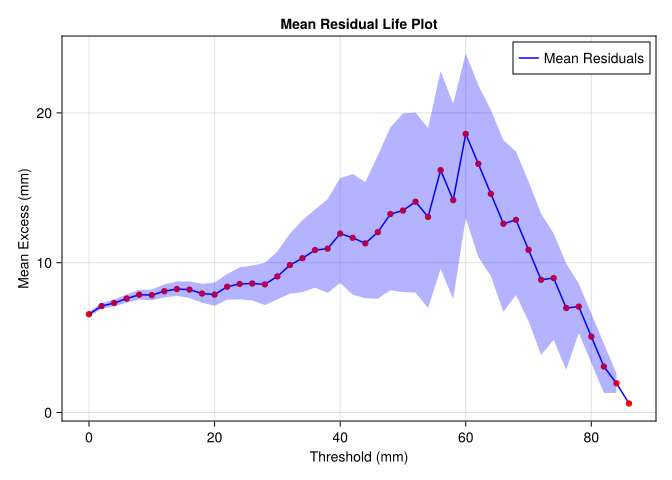
\includegraphics[keepaspectratio]{index_files/mediabag/chapters/hazard/extremes_files/figure-latex/..-..-notebooks-block-maxima-fig-mean-residual-life-output-1.pdf}}

}

\caption{\label{fig-mean-residual-life}Mean Residual Life Plot for
extreme rainfall data}

\end{figure}%

\begin{figure}

\centering{

\pandocbounded{\includegraphics[keepaspectratio]{index_files/mediabag/chapters/hazard/extremes_files/figure-latex/..-..-notebooks-sewells-point-fig-return-scatter-output-1.pdf}}

}

\caption{\label{fig-return-scatter}Return Period with Uncertainty}

\end{figure}%

\subsection{Parameter Estimation}\label{parameter-estimation}

Several approaches exist for fitting extreme value distributions:

\subsubsection{Maximum Likelihood Estimation
(MLE)}\label{maximum-likelihood-estimation-mle}

\textbf{Most common approach}: Find parameters that maximize likelihood
of observed data

\textbf{Advantages}: - Asymptotically efficient and unbiased - Provides
uncertainty estimates via Fisher information - Standard statistical
inference procedures apply

\textbf{Disadvantages}: - Can be unstable for small samples - May not
exist for some parameter combinations - Sensitive to outliers

\subsubsection{Probability Weighted Moments
(PWM)}\label{probability-weighted-moments-pwm}

\textbf{Alternative approach}: Match theoretical and sample probability
weighted moments

\textbf{Advantages}: - Often more robust than MLE for small samples -
Computationally simpler - Less sensitive to outliers

\textbf{Disadvantages}: - Less efficient than MLE asymptotically -
Uncertainty quantification more complex

\subsubsection{Bayesian Methods}\label{bayesian-methods}

\textbf{Modern approach}: Specify prior distributions and compute
posterior

\textbf{Advantages}: - Natural uncertainty quantification - Can
incorporate prior knowledge - Regularizes parameter estimates - Handles
model selection coherently

\textbf{Disadvantages}: - Requires prior specification - Computationally
intensive - Results depend on prior choice

\section{Challenges in Extreme Value
Analysis}\label{challenges-in-extreme-value-analysis}

\subsection{Parametric Uncertainty}\label{parametric-uncertainty}

\textbf{Problem}: Many parameter values consistent with limited extreme
data \textbf{Consequence}: Very different conclusions about rare event
probabilities \textbf{Example}: Shape parameter uncertainty leads to
large confidence intervals for return levels

\textbf{Management approaches}: - Bayesian methods for uncertainty
quantification - Regional information to stabilize estimates -
Informative priors based on physical understanding

\subsection{Model Structure
Uncertainty}\label{model-structure-uncertainty}

\textbf{Problem}: Different distributional assumptions yield different
results \textbf{Common comparisons}: - GEV vs.~alternative distributions
(Log-Pearson III, etc.) - Stationary vs.~non-stationary models - Block
maxima vs.~POT approaches

\textbf{Management approaches}: - Information criteria for model
selection - Model averaging across plausible alternatives - Sensitivity
analysis across model choices

\subsection{Sampling Uncertainty}\label{sampling-uncertainty}

\textbf{Problem}: Finite samples for rare event estimation \textbf{Key
insight}: If Hurricane Harvey had never occurred, 100-year rainfall
estimates would be very different

\textbf{Implications}: - Confidence intervals grow rapidly with return
period - Need for longer records or supplementary information - Regional
pooling to increase effective sample size

\section{Non-Stationarity and Climate
Change}\label{non-stationarity-and-climate-change-1}

\textbf{Traditional assumption}: Statistical properties constant over
time \textbf{Climate reality}: Extreme value characteristics changing
due to: - Rising temperatures affecting heat extremes - Changing
precipitation patterns - Shifting storm tracks and intensity - Sea level
rise affecting coastal extremes

\subsection{Covariate Methods}\label{covariate-methods}

Allow extreme value parameters to depend on covariates:

\[\mu(t) = \mu_0 + \mu_1 \cdot \text{covariate}(t)\]

\textbf{Common covariates}: - Time trends (linear, polynomial) - Climate
indices (ENSO, AMO) - Global temperature anomalies - Physical process
variables

\textbf{Benefits}: Called ``process-informed'' approaches (Schlef et al.
2023) \textbf{Reviews}: See Salas, Obeysekera, and Vogel (2018) for
comprehensive treatment

\subsection{Implementation Challenges}\label{implementation-challenges}

\begin{itemize}
\tightlist
\item
  \textbf{Model selection}: Which covariates to include?
\item
  \textbf{Functional form}: Linear vs.~nonlinear relationships?
\item
  \textbf{Parameter dependence}: Which parameters vary with covariates?
\item
  \textbf{Prediction}: How to project covariates into future?
\end{itemize}

\subsection{Practical Considerations}\label{practical-considerations}

\textbf{Design implications}: Traditional return period concept breaks
down \textbf{Risk assessment}: Need for time-varying risk measures
\textbf{Decision-making}: Robust strategies under non-stationarity

\section{Non-Stationary Extreme Value Analysis: Theory and
Practice}\label{non-stationary-extreme-value-analysis-theory-and-practice}

\subsection{The Stationarity Assumption and Its
Breakdown}\label{the-stationarity-assumption-and-its-breakdown}

Extreme value theory is based on the assumption that the data are
independent and identically distributed (iid): - Each draw comes from
the same distribution - Statistical properties remain constant over time

This assumption is violated by: - Climate change effects on temperature
and precipitation extremes - Low-frequency variability (e.g., Pacific
Decadal Oscillation) - Memory processes in the climate system -
Urbanization and land use changes

\subsection{What is Stationarity?}\label{what-is-stationarity}

A stationary process is a stochastic process whose unconditional joint
probability distribution does not change when shifted in time. A
stochastic process is a model for a \emph{sequence} of random variables
(e.g., random walk, MCMC).

As famously stated by Milly et al. (2008): ``Stationarity is dead.''

\subsection{Climate Change Impacts on
Extremes}\label{climate-change-impacts-on-extremes}

\textbf{Thermodynamic Effects:} - Clausius-Clapeyron relation:
\(e_s(T) = e_0 \exp\left(\frac{L_v}{R_v T}\right)\) - Approximately 7\%
increase in atmospheric moisture per degree K of warming - Direct
impacts on precipitation intensity

\textbf{Dynamic Effects:} - Longer, hotter summers due to slower
seasonal transitions - Poleward expansion of tropical circulation
patterns - Changes in storm structure and intensity - Shifts in jet
stream patterns affecting extreme weather

The following content draws from Seneviratne et al. (2021) executive
summary:

\textbf{Climate Change Impacts on Precipitation:} - The frequency and
intensity of heavy precipitation events have likely increased at the
global scale over a majority of land regions with good observational
coverage - Heavy precipitation has likely increased on the continental
scale over three continents: North America, Europe, and Asia - Heavy
precipitation will generally become more frequent and more intense with
additional global warming - At a global warming level of 4°C relative to
the pre-industrial level, very rare (e.g., one in 10 or more years)
heavy precipitation events would become more frequent and more intense
than in the recent past, on the global scale (virtually certain) and in
all continents and AR6 regions - The projected increase in the intensity
of extreme precipitation translates to an increase in the frequency and
magnitude of pluvial floods -- surface water and flash floods -- (high
confidence)

\textbf{Climate Change Impacts on River Floods:} - Significant trends in
peak streamflow have been observed in some regions over the past decades
(high confidence) - The seasonality of river floods has changed in cold
regions where snow-melt is involved, with an earlier occurrence of peak
streamflow (high confidence) - Global hydrological models project a
larger fraction of land areas to be affected by an increase in river
floods than by a decrease in river floods (medium confidence)

\textbf{Climate Change Impacts on Extreme Temperatures:} - The frequency
and intensity of hot extremes (including heatwaves) have increased, and
those of cold extremes have decreased on the global scale since 1950
(virtually certain) - Human-induced greenhouse gas forcing is the main
driver of the observed changes in hot and cold extremes on the global
scale (virtually certain) and on most continents (very likely) - The
frequency and intensity of hot extremes will continue to increase and
those of cold extremes will continue to decrease, at global and
continental scales and in nearly all inhabited regions with increasing
global warming levels

\textbf{Climate Change Impacts on Tropical Cyclones:} - The average and
maximum rain rates associated with tropical cyclones (TCs),
extratropical cyclones and atmospheric rivers across the globe, and
severe convective storms in some regions, increase in a warming world
(high confidence) - It is likely that the global proportion of Category
3--5 tropical cyclone instances has increased over the past four decades
- The proportion of intense TCs, average peak TC wind speeds, and peak
wind speeds of the most intense TCs will increase on the global scale
with increasing global warming (high confidence) - Future wind speed
changes are expected to be small, although poleward shifts in the storm
tracks could lead to substantial changes in extreme wind speeds in some
regions (medium confidence)

\textbf{El Niño-Southern Oscillation Effects:} El Niño-Southern
Oscillation remains a major driver of interannual climate variability,
affecting extreme value statistics through teleconnections that modify
regional precipitation and temperature patterns.

\subsection{Non-Stationary Modeling
Approaches}\label{non-stationary-modeling-approaches}

\textbf{Rolling Window Approach:} - Simple method that estimates
parameters using moving time windows - \textbf{Advantages}: Simple and
interpretable - \textbf{Disadvantages}: Noisy estimates, potential loss
of extreme events at window boundaries - Less bias but more variance
compared to stationary models

\textbf{Regression Models for Parameters:} In linear regression and
GLMs, every data point is drawn from its own distribution that depends
on parameters and covariates. We can apply this approach to extreme
value models by allowing GEV or GPD parameters to vary with covariates.

\textbf{Types of Parameter Variation:} What can vary with
time/covariates? 1. Location parameter: \(\mu(t) = f(X(t))\) 2. Scale
parameter: \(\sigma(t) = f(X(t))\) 3. Both location and scale parameters
4. Scale and coefficient of variation: \(\mu(t) = \phi \sigma(t)\) 5.
Varying shape parameter (impractical but theoretically allowed)

\textbf{Functional Forms for Parameter Variation:} How parameters vary
with covariates: 1. Linear relationships:
\(\theta(t) = \alpha + \beta_1 X_1(t) + \beta_2 X_2(t) + \cdots\) 2.
Nonlinear relationships using splines, GAMs, or other flexible
approaches 3. Anything is theoretically allowed, but not everything is
practical for extreme value analysis

\subsection{Covariate Selection}\label{covariate-selection}

\textbf{General Guidance:} - Physical theory and domain knowledge are
invaluable for covariate selection - For precipitation extremes,
logarithm of CO2 concentration is often a useful covariate because: - It
isolates the global warming signal from natural variability like ENSO -
It provides a monotonic trend that matches expected thermodynamic
responses

\textbf{Common Covariates:} - Time (linear or polynomial trends) -
Global mean temperature anomalies - Logarithm of atmospheric CO2
concentration - Climate oscillation indices (ENSO, AMO, PDO) - Local
environmental variables (sea surface temperatures, soil moisture)

\subsection{Case Study: Houston Hobby Airport Precipitation
Analysis}\label{case-study-houston-hobby-airport-precipitation-analysis}

\textbf{Motivation:} Analysis of trends in extreme precipitation at
Houston Hobby Airport demonstrates practical implementation of
non-stationary extreme value methods.

\textbf{Data Considerations:} - Annual maximum daily precipitation from
NOAA GHCND - Quality control: keep only years with at least 350 days of
data - Need to address potential non-stationarity due to climate change

\textbf{Trend Analysis:} The Mann-Kendall test is commonly used to
assess the presence of trends in time series data. Rank correlation
between precipitation ranks and years provides initial evidence of
trends.

\textbf{Model Formulations:}

\emph{Location Trend Model:} \[
\begin{aligned}
y_t &\sim \text{GEV} \left( \mu_t, \sigma, \xi \right) \\
\mu_t &= \alpha + \beta X_t
\end{aligned}
\]

\emph{Scale Trend Model:} \[
\begin{aligned}
y_t &\sim \text{GEV} \left( \mu, \sigma_t, \xi \right) \\
\log(\sigma_t) &= \alpha + \beta X_t
\end{aligned}
\]

\emph{Combined Location and Scale Trend:} \[
\begin{aligned}
y_t &\sim \text{GEV} \left( \mu_t, \sigma_t, \xi \right) \\
\mu_t &= \alpha_\mu + \beta_\mu X_t \\
\log(\sigma_t) &= \alpha_\sigma + \beta_\sigma X_t
\end{aligned}
\]

\subsection{Implementation
Considerations}\label{implementation-considerations}

\textbf{Computational Tools:} - \texttt{Extremes.jl} package provides
\texttt{gevfitbayes()} function with covariate support - Can specify
\texttt{locationcovid} and \texttt{logscalecovid} parameters for
regression modeling - Default uniform priors may not be ideal - custom
priors often needed

\textbf{Model Comparison:} Comparison between stationary and various
non-stationary models helps identify: - Which parameters are most
sensitive to climate change - How return level estimates change with
different trend assumptions - Uncertainty in future projections under
continued warming

\subsection{Key Insights from Non-Stationary
Analysis}\label{key-insights-from-non-stationary-analysis}

\textbf{Bias-Variance Trade-off:} - Non-stationary models reduce bias by
accounting for trends - But increase variance due to additional
parameters to estimate - Physical process knowledge helps guide model
selection

\textbf{Parametric Uncertainty:} - Non-stationary models typically have
larger parametric uncertainty - Future projections require assumptions
about covariate evolution - Model comparison becomes even more critical

\textbf{Practical Implications:} - Traditional design standards may need
updating - Infrastructure planning must account for changing risk
profiles - Adaptive management strategies become more important

\section{Regionalization and Spatial
Methods}\label{regionalization-and-spatial-methods}

\textbf{Motivation}: Single-site records often too short for reliable
extreme value analysis

Nearby stations should (usually) have similar precipitation, flood, or
other extreme event probabilities. Regionalization methods reduce
estimation error by pooling information while reducing sampling error
from random variation between nearby stations. However, regionalization
does NOT reduce sampling error from major regional events that affect
all stations simultaneously.

\subsection{Classical Regional Frequency
Analysis}\label{classical-regional-frequency-analysis}

\textbf{L-Moment Estimators:} L-moments are linear combinations of order
statistics that can be used to match theoretical and empirical
distribution moments.

\textbf{Advantages}: - Computationally efficient - Work well in practice
- Robust parameter estimation

\textbf{Disadvantages}: - Less flexible than likelihood-based methods -
Difficult to quantify parametric uncertainty - Limited ability to
incorporate covariates

\textbf{Regional Frequency Analysis Process:} 1. \textbf{Assign sites to
regions} based on climate, geography, or other similarity measures 2.
\textbf{Estimate L-moments for each site} using observed data 3.
\textbf{Check for regional homogeneity} using statistical tests 4.
\textbf{Take regional L-moments} as the weighted mean of site L-moments
5. \textbf{Apply scaling factors} (e.g., average annual maximum flood
for each site)

This approach is best implemented using the R \texttt{lmomRFA} package,
which can be called from Julia using \texttt{RCall.jl}.

\subsection{Region of Influence
Approach}\label{region-of-influence-approach}

\textbf{Motivation:} RFA assumes all sites are assigned to a single
region, but often regions are not distinct.

\textbf{Methodology:} 1. \textbf{Define similarity measures} between
each pair of sites (e.g., distance, land use, elevation, climate
indices) 2. \textbf{For estimates at site i}, define its ``region of
influence'' as the most similar sites (analogous to k-nearest neighbors)
3. \textbf{Estimate L-moments} for each site and compute weighted
average as in RFA 4. \textbf{Allow flexible, site-specific regions}
rather than rigid regional boundaries

\textbf{Advantages}: - More flexible than traditional RFA - Can adapt
region definition to local characteristics - Better handles sites near
regional boundaries

\subsection{Hierarchical Bayesian
Models}\label{hierarchical-bayesian-models}

Modern spatial approaches use hierarchical models to balance between
``full pooling'' (all sites identical) and ``no pooling'' (each site
independent).

\subsection{Full Pooling Approach}\label{full-pooling-approach}

\textbf{Concept}: Assume within a region, all sites have the same
distribution. Estimate a single distribution for the entire region. This
is analogous to classical regional frequency analysis.

\textbf{Bayesian Implementation:}

\begin{Shaded}
\begin{Highlighting}[]
\PreprocessorTok{@model} \KeywordTok{function} \FunctionTok{gev\_fully\_pooled}\NormalTok{(y}\OperatorTok{::}\DataTypeTok{AbstractMatrix}\NormalTok{)}
\NormalTok{    N\_yr, N\_stn }\OperatorTok{=} \FunctionTok{size}\NormalTok{(y)}
\NormalTok{    μ }\OperatorTok{\textasciitilde{}} \FunctionTok{Normal}\NormalTok{(}\FloatTok{5}\NormalTok{, }\FloatTok{5}\NormalTok{)}
\NormalTok{    σ }\OperatorTok{\textasciitilde{}} \FunctionTok{LogNormal}\NormalTok{(}\FloatTok{0}\NormalTok{, }\FloatTok{2}\NormalTok{)}
\NormalTok{    ξ }\OperatorTok{\textasciitilde{}} \FunctionTok{Uniform}\NormalTok{(}\OperatorTok{{-}}\FloatTok{0.5}\NormalTok{, }\FloatTok{0.5}\NormalTok{)}
    \ControlFlowTok{for}\NormalTok{ s }\KeywordTok{in} \FloatTok{1}\OperatorTok{:}\NormalTok{N\_stn}
        \ControlFlowTok{for}\NormalTok{ t }\KeywordTok{in} \FloatTok{1}\OperatorTok{:}\NormalTok{N\_yr}
            \ControlFlowTok{if}\NormalTok{ !}\FunctionTok{ismissing}\NormalTok{(y[t, s])}
\NormalTok{                y[t, s] }\OperatorTok{\textasciitilde{}} \FunctionTok{GeneralizedExtremeValue}\NormalTok{(μ, σ, ξ)}
            \ControlFlowTok{end}
        \ControlFlowTok{end}
    \ControlFlowTok{end}
\KeywordTok{end}
\end{Highlighting}
\end{Shaded}

\textbf{Advantages}: - Fast sampling due to high data-to-parameter ratio
- Simple to implement and interpret - Maximizes information sharing
across sites

\textbf{Important Limitation}: This approach weights each observation
equally, regardless of site or year. If some years have more
observations than others, those years are implicitly weighted more
heavily. A better model would weight each year equally.

\subsection{Partial Pooling Approach}\label{partial-pooling-approach}

\textbf{Concept}: Model parameters at each site as being drawn from a
common distribution. This balances between full pooling and no pooling
by sharing information while allowing site-specific variation.

\textbf{Mathematical Framework:} \[
\begin{aligned}
    y_{s,t} &\sim \text{GEV}(\mu_s, \sigma_s, \xi_s) \\
    \mu_s &\sim \text{Normal}(\mu^0, \tau^\mu) \\
    \sigma_s &\sim \text{LogNormal}(\sigma^0, \tau^\sigma) \\
    \xi &\sim \text{Uniform}(-0.5, 0.5) \text{ (fully pooled)}
\end{aligned}
\]

where \(s\) is the site index and \(t\) is the year index.

\textbf{Hyperparameters}: In Bayesian statistics, hyperparameters like
\(\mu^0\) and \(\tau^\mu\) are learned as part of the model. These
describe the distribution from which site-specific parameters are drawn.

\textbf{Implementation Example:}

\begin{Shaded}
\begin{Highlighting}[]
\PreprocessorTok{@model} \KeywordTok{function} \FunctionTok{gev\_partial\_pool}\NormalTok{(y}\OperatorTok{::}\DataTypeTok{AbstractMatrix}\NormalTok{)}
\NormalTok{    N\_yr, N\_stn }\OperatorTok{=} \FunctionTok{size}\NormalTok{(y)}

    \CommentTok{\# Define hyperparameters with informative priors}
\NormalTok{    μ₀ }\OperatorTok{\textasciitilde{}} \FunctionTok{Normal}\NormalTok{(}\FloatTok{5}\NormalTok{, }\FloatTok{3}\NormalTok{)}
\NormalTok{    τμ }\OperatorTok{\textasciitilde{}} \FunctionTok{LogNormal}\NormalTok{(}\FloatTok{0}\NormalTok{, }\FloatTok{0.5}\NormalTok{)}
\NormalTok{    σ₀ }\OperatorTok{\textasciitilde{}} \FunctionTok{LogNormal}\NormalTok{(}\FloatTok{0.5}\NormalTok{, }\FloatTok{0.5}\NormalTok{)}
\NormalTok{    τσ }\OperatorTok{\textasciitilde{}} \FunctionTok{LogNormal}\NormalTok{(}\FloatTok{0}\NormalTok{, }\FloatTok{0.5}\NormalTok{)}

    \CommentTok{\# Site{-}specific parameters depend on hyperparameters}
\NormalTok{    μ }\OperatorTok{\textasciitilde{}} \FunctionTok{filldist}\NormalTok{(}\FunctionTok{Normal}\NormalTok{(μ₀, τμ), N\_stn)}
\NormalTok{    σ }\OperatorTok{\textasciitilde{}} \FunctionTok{filldist}\NormalTok{(}\FunctionTok{truncated}\NormalTok{(}\FunctionTok{Normal}\NormalTok{(σ₀, τσ), }\FloatTok{0}\NormalTok{, }\ConstantTok{Inf}\NormalTok{), N\_stn)}

    \CommentTok{\# Fully pooled shape parameter}
\NormalTok{    ξ }\OperatorTok{\textasciitilde{}} \FunctionTok{Uniform}\NormalTok{(}\OperatorTok{{-}}\FloatTok{0.5}\NormalTok{, }\FloatTok{0.5}\NormalTok{)}

    \CommentTok{\# Likelihood}
    \ControlFlowTok{for}\NormalTok{ s }\KeywordTok{in} \FloatTok{1}\OperatorTok{:}\NormalTok{N\_stn}
        \ControlFlowTok{for}\NormalTok{ t }\KeywordTok{in} \FloatTok{1}\OperatorTok{:}\NormalTok{N\_yr}
\NormalTok{            y[t, s] }\OperatorTok{\textasciitilde{}} \FunctionTok{GeneralizedExtremeValue}\NormalTok{(μ[s], σ[s], ξ)}
        \ControlFlowTok{end}
    \ControlFlowTok{end}
\KeywordTok{end}
\end{Highlighting}
\end{Shaded}

\textbf{Computational Considerations}: With \(N\) stations, we have
\(4 + N + N + 1 = 5 + 2N\) parameters to estimate, making sampling
slower than full pooling. Careful prior specification becomes more
important with increased model complexity.

\subsection{Spatial Regression Models}\label{spatial-regression-models}

\textbf{Alternative Approach}: Model parameters as functions of
geographical location and environmental covariates. This can simplify
the model by reducing the number of parameters to estimate.

\textbf{Simple Spatial Model Example:} \[
\begin{aligned}
    \mu(s) &= \alpha^\mu + \beta^\mu_1 \cdot \text{lat}(s) + \beta^\mu_2 \cdot \text{lon}(s) \\
    \sigma(s) &= \alpha^\sigma + \beta^\sigma_1 \cdot \text{lat}(s) + \beta^\sigma_2 \cdot \text{lon}(s) \\
    y_{s,t} &\sim \text{GEV}(\mu(s), \sigma(s), \xi)
\end{aligned}
\]

\textbf{Extensions}: - Include elevation, distance to coast, climate
indices as covariates - Use flexible relationships (splines, GAMs)
instead of linear functions - Incorporate spatial correlation through
Gaussian process priors - Combine with temporal trends for
spatiotemporal modeling

\subsection{Practical Implementation
Considerations}\label{practical-implementation-considerations}

\textbf{Data Challenges:} - Missing data requires careful treatment in
likelihood calculations - Different record lengths across sites - Need
for quality control and homogenization

\textbf{Model Selection:} - Compare full pooling, partial pooling, and
no pooling approaches - Use cross-validation or information criteria -
Consider out-of-sample prediction performance

\textbf{Uncertainty Quantification:} - Hierarchical models naturally
provide uncertainty estimates - Can propagate parameter uncertainty to
return level calculations - Important for decision-making under
uncertainty

\subsection{Regional Frequency
Analysis}\label{regional-frequency-analysis}

\textbf{Approach}: Pool information across ``similar'' sites

\begin{enumerate}
\def\labelenumi{\arabic{enumi}.}
\tightlist
\item
  \textbf{Identify regions}: Group sites with similar extreme value
  behavior
\item
  \textbf{Normalize data}: Scale to common distribution
\item
  \textbf{Fit regional model}: Estimate shape parameter regionally
\item
  \textbf{Scale back}: Apply regional parameters to individual sites
\end{enumerate}

\textbf{Advantages}: - Increased effective sample size - More stable
parameter estimates - Better extrapolation to rare events

\textbf{Challenges}: - Defining hydrologically similar regions - Testing
regional homogeneity - Accounting for cross-site dependence

\subsection{Modern Spatial Approaches}\label{modern-spatial-approaches}

\textbf{Hierarchical models}: Borrow strength across space while
allowing local variation \textbf{Spatial random effects}: Model spatial
correlation in extreme value parameters \textbf{Machine learning}: Use
environmental covariates to predict extreme value parameters

\section{Case Studies}\label{case-studies}

\subsection{Hurricane Harvey and the Addicks/Barker
Reservoirs}\label{hurricane-harvey-and-the-addicksbarker-reservoirs}

\textbf{Context}: Legal case requiring extreme precipitation frequency
analysis

\textbf{Challenges}: - Interacting drivers of non-stationarity - Short
observational records - High stakes for affected communities

\textbf{Key insights}: - Plausible assumptions led to vastly different
estimates - No single ``objective'' answer exists - Uncertainty
quantification crucial for decision-making

\subsection{Texas Precipitation Frequency
Analysis}\label{texas-precipitation-frequency-analysis}

\textbf{Project}: Joint TWDB/TAMU/Rice effort to update Atlas 14

\textbf{Motivation}: - NOAA Atlas 14 doesn't account for climate change
- Need state-wide consistent methodology - Multiple durations and return
periods required

\textbf{Approach}: - More stations than federal analysis - Climate
change considerations - Advanced uncertainty quantification

\subsection{Winter Storm Uri Analysis}\label{winter-storm-uri-analysis}

\textbf{Questions}: How likely was this event? Should we have been
prepared?

\textbf{Variables studied}: - Temperature at individual grid cells -
Population-weighted temperature indices - Duration and spatial extent

\textbf{Findings}: Illustrated challenges of: - Compound extremes (cold
+ widespread) - Infrastructure vulnerability to rare events - Need for
robust planning under uncertainty

\section{Computational Tools}\label{computational-tools}

\textbf{R packages}: - \texttt{ismev}: Classical extreme value methods -
\texttt{evd}: Extended extreme value distributions - \texttt{POT}:
Peak-over-threshold methods

\textbf{Julia packages}: - \texttt{Extremes.jl}: Comprehensive extreme
value toolkit - Well-documented with practical examples

\textbf{Python packages}: - \texttt{scipy.stats}: Basic extreme value
distributions - \texttt{pyextremes}: Specialized extreme value analysis

\section*{Further reading}\label{further-reading-7}
\addcontentsline{toc}{section}{Further reading}

\markright{Further reading}

\textbf{Essential texts}: - Coles (2001): Canonical extreme value
textbook with mathematical rigor and practical examples

\textbf{Current research directions}: - Sampling uncertainty: Lu, Seiyon
Lee, and Doss-Gollin (2025) discusses spatial approaches -
Non-independence: Accounting for temporal and spatial dependence -
Climate change: Non-stationary extreme value models - Machine learning:
Neural networks for extreme value analysis - Multivariate extremes:
Joint behavior of multiple variables

\chapter{Downscaling and Bias Correction
✏️}\label{downscaling-and-bias-correction}

\section*{See first}\label{see-first-6}
\addcontentsline{toc}{section}{See first}

\markright{See first}

This chapter builds on concepts from: -
\href{./chapters/fundamentals/climate-science.qmd}{Fundamentals of
Climate Science} -
\href{./chapters/fundamentals/correlation-dimensionality.qmd}{Correlation
and Dimensionality}

\section*{Learning objectives}\label{learning-objectives-8}
\addcontentsline{toc}{section}{Learning objectives}

\markright{Learning objectives}

After reading this chapter, you should be able to:

\begin{itemize}
\tightlist
\item
  Distinguish between supervised and distributional downscaling
  approaches
\item
  Understand the motivation for downscaling climate model outputs
\item
  Apply bias correction and quantile-quantile mapping techniques
\item
  Recognize the stationarity assumption and its implications
\item
  Evaluate different downscaling methods for specific applications
\item
  Understand modern machine learning approaches to climate downscaling
\end{itemize}

\section{Motivation}\label{motivation}

Climate models operate at coarse spatial and temporal resolutions, but
many applications require high-resolution climate information:

\begin{itemize}
\tightlist
\item
  \textbf{Stormwater management}: Long-term design requires hourly
  precipitation at city scales
\item
  \textbf{Water resources management}: Subseasonal to multi-year
  planning needs basin-specific information
\item
  \textbf{Fire propagation}: Hourly to weekly meteorological conditions
  at landscape scales
\item
  \textbf{Agriculture}: Daily temperature and precipitation at field
  scales
\end{itemize}

\subsection{Objectives of Downscaling}\label{objectives-of-downscaling}

Downscaling aims to achieve three primary objectives (Lanzante et al.
2018):

\begin{enumerate}
\def\labelenumi{\arabic{enumi}.}
\tightlist
\item
  \textbf{Enhanced spatial detail}: Increase resolution from
  \textasciitilde100-200 km to \textasciitilde1-10 km
\item
  \textbf{Mitigation of systematic ESM biases}: Correct known model
  biases
\item
  \textbf{Generation of variables not explicitly rendered by GCMs}:
  Derive additional variables
\end{enumerate}

\subsection{Challenges with Earth System
Models}\label{challenges-with-earth-system-models}

Earth System Models (ESMs) face inherent limitations for local
applications:

\begin{enumerate}
\def\labelenumi{\arabic{enumi}.}
\tightlist
\item
  \textbf{Scale mismatch}: ESMs are tuned for energy balance and
  large-scale circulation, not local extremes
\item
  \textbf{Spatial averaging}: Grid cells represent averages over large
  areas
\item
  \textbf{Temporal averaging}: Time steps may miss sub-daily variability
\item
  \textbf{Process representation}: Local-scale processes may be
  parameterized or missing
\end{enumerate}

Two specific challenges illustrate these limitations:

\begin{itemize}
\tightlist
\item
  \textbf{``Dreary'' problem}: Models produce too many days with light
  precipitation
\item
  \textbf{``Drizzling'' problem}: Models fail to capture intense
  precipitation events
\end{itemize}

These systematic biases require correction for practical applications.

\section{Supervised Methods}\label{supervised-methods}

Supervised downscaling is especially common in weather forecasting,
where we have pairs of (observed, forecasted) data.

\subsection{Framework}\label{framework}

Supervised downscaling treats the problem as a statistical learning
task:

\begin{itemize}
\tightlist
\item
  \textbf{Input}: Pairs \((X_i, y_i)\) where:

  \begin{itemize}
  \tightlist
  \item
    \(X_i\): Predictors (e.g., gridded model output)
  \item
    \(y_i\): Predictand (e.g., station observations)
  \end{itemize}
\item
  \textbf{Goal}: Learn function \(f\) such that \(f(X_i) \approx y_i\)
\item
  \textbf{Key requirement}: \(X_i\) and \(y_i\) observed at the same
  time
\end{itemize}

Quality is measured through loss functions (e.g., mean squared error,
likelihood).

\subsection{Applications}\label{applications-2}

Supervised methods work well when: - Historical model-observation pairs
exist - Relationship between predictors and predictand is stable - Focus
is on weather forecasting or hindcasting

\textbf{Examples}: - Mapping satellite to radar precipitation data -
Post-processing numerical weather predictions - Downscaling reanalysis
to station observations

\subsection{Example: Linear
Regression}\label{example-linear-regression-1}

Simplest approach relates large-scale predictors to local observations:

\[y = \beta_0 + \sum_{j=1}^p \beta_j X_j + \epsilon\]

where \(X_j\) might include: - Temperature at multiple pressure levels -
Geopotential height gradients - Humidity measures - Previous day's local
weather

\textbf{Advantages}: Simple, interpretable, computationally fast
\textbf{Limitations}: Assumes linear relationships, may miss complex
interactions

\subsection{Example: Model Output Statistics
(MOS)}\label{example-model-output-statistics-mos}

Operational approach used by weather services:

\begin{enumerate}
\def\labelenumi{\arabic{enumi}.}
\tightlist
\item
  \textbf{Preprocessing}: Standardize model outputs and observations
\item
  \textbf{Predictor selection}: Choose relevant large-scale variables
\item
  \textbf{Model fitting}: Often multiple linear regression with
  categorical predictors
\item
  \textbf{Post-processing}: Apply adjustments for known biases
\end{enumerate}

\textbf{Key insight}: MOS exploits systematic model biases to improve
forecasts.

\subsection{Example: Generative ML}\label{example-generative-ml}

Modern approach using deep learning:

\begin{itemize}
\tightlist
\item
  \textbf{Generative Adversarial Networks (GANs)}: Learn to generate
  realistic high-resolution fields
\item
  \textbf{Diffusion models}: Model the data generation process through
  noise injection and removal
\item
  \textbf{Conditional models}: Generate outputs conditional on
  large-scale inputs
\end{itemize}

\textbf{Goal}: Sample from \(p(y|X)\) rather than just predict
\(\mathbb{E}[y|X]\)

\textbf{Advantages}: Can capture complex nonlinear relationships and
full probability distributions \textbf{Limitations}: Computationally
intensive, requires large training datasets, difficult to interpret

\section{Distribution-Based Methods}\label{distribution-based-methods}

\subsection{The Climate Model
Challenge}\label{the-climate-model-challenge}

Climate models present a unique challenge different from weather
forecasting. ESMs simulate from the distribution of weather given
climate boundary conditions:

\begin{itemize}
\tightlist
\item
  Run 100 ESM ensemble members over historical conditions
\item
  Study December 1, 1980 across all ensemble members
\item
  Some realizations will be rainy, others dry; some cool, others warm
\item
  \textbf{Statistically meaningful but not deterministic forecasts}
\end{itemize}

\subsection{No Paired Data Problem}\label{no-paired-data-problem}

Unlike weather forecasting, climate models don't provide paired
observations: - We have samples \({X_1, \ldots, X_N}\) from climate
model - We have samples \({y_1, \ldots, y_K}\) from observations - No
correspondence between \(X_i\) and \(y_j\) at specific times

\textbf{Key insight}: April 15, 1995 in model ≠ April 15, 1995 in
observations

Both are samples from ``distribution of late April weather in 1990s
conditions''

\subsection{Distributional Approach}\label{distributional-approach}

Since we cannot use supervised methods, we compare distributions:

\[p_{\text{model}}(X) \neq p_{\text{obs}}(y)\]

Goal: Transform model outputs to match observational distribution
characteristics.

\subsection{Example: Bias Correction}\label{example-bias-correction}

Simplest distributional method corrects the mean:

\[\begin{aligned}
\text{bias} &= \mathbb{E}[X] - \mathbb{E}[y] \\
\hat{y} &= X - \text{bias}
\end{aligned}\]

\textbf{Question}: Is this distributional or supervised?
\textbf{Answer}: Distributional - uses distributional moments, not
paired data.

\subsection{Example: Quantile-Quantile
Mapping}\label{example-quantile-quantile-mapping}

More sophisticated approach matching full distributions:

\begin{enumerate}
\def\labelenumi{\arabic{enumi}.}
\item
  \textbf{Calculate quantiles}: For probabilities \(p \in [0,1]\):

  \begin{itemize}
  \tightlist
  \item
    Model quantile: \(q_m(p) = F_m^{-1}(p)\)
  \item
    Observed quantile: \(q_o(p) = F_o^{-1}(p)\)
  \end{itemize}
\item
  \textbf{Create mapping function}: \(h(x) = F_o^{-1}(F_m(x))\)
\item
  \textbf{Apply correction}: \(\hat{y} = h(X)\)
\end{enumerate}

\textbf{Interpretation}: Transform model value to its quantile, then map
to corresponding observed quantile.

\textbf{Advantages}: - Corrects entire distribution, not just mean -
Preserves temporal correlations - Handles non-Gaussian distributions

\textbf{Limitations}: - Assumes stationarity of correction - Cannot add
variability not present in model - May create artifacts at distribution
tails

\subsection{Example: CDF Matching}\label{example-cdf-matching}

Alternative approach directly matches cumulative distribution functions:

\begin{enumerate}
\def\labelenumi{\arabic{enumi}.}
\tightlist
\item
  \textbf{Estimate CDFs}: \(\hat{F}_m(x)\) and \(\hat{F}_o(x)\)
\item
  \textbf{Define mapping}: Minimize
  \(\int |\hat{F}_m(h(x)) - \hat{F}_o(x)| dx\)
\item
  \textbf{Apply transformation}: Use optimal \(h(\cdot)\) to correct
  future data
\end{enumerate}

This is closely related to quantile mapping but may use different
estimation techniques.

\section{Advanced Machine Learning
Approaches}\label{advanced-machine-learning-approaches}

\subsection{CorrectorGAN}\label{correctorgan}

Recent work applies Generative Adversarial Networks to bias correction
(Price and Rasp 2022):

\textbf{Architecture}: - \textbf{Generator}: Takes coarse model output,
produces high-resolution corrected field - \textbf{Discriminator}:
Learns to distinguish real observations from generated corrections

\textbf{Advantages}: - Learns complex spatial patterns - Can generate
multiple plausible realizations - Captures spatial correlations better
than pointwise methods

\textbf{Training process}: 1. Generator learns mapping from model to
observations 2. Discriminator learns to identify ``realistic'' weather
patterns 3. Adversarial training improves both networks

\subsection{Other Modern Approaches}\label{other-modern-approaches}

\textbf{Super-resolution methods}: Increase spatial resolution while
correcting biases \textbf{Conditional diffusion models}: Generate
high-resolution weather conditioned on large-scale patterns
\textbf{Physics-informed neural networks}: Incorporate physical
constraints into ML models

\section{Dynamical Downscaling}\label{dynamical-downscaling}

\subsection{Physics-Based Dynamical
Downscaling}\label{physics-based-dynamical-downscaling}

\textbf{Approach}: Run high-resolution regional climate model (RCM)
nested within global model:

\begin{enumerate}
\def\labelenumi{\arabic{enumi}.}
\tightlist
\item
  \textbf{Global model} provides boundary conditions
\item
  \textbf{Regional model} simulates detailed physics at
  \textasciitilde10-50 km resolution
\item
  \textbf{Output} includes all meteorological variables at high
  resolution
\end{enumerate}

\textbf{Advantages}: - Physically consistent - Captures local
topographic effects - Generates all meteorological variables
simultaneously

\textbf{Limitations}: - Computationally expensive - May inherit global
model biases - Still requires bias correction for many applications

\subsection{AI-Based Dynamical
Downscaling}\label{ai-based-dynamical-downscaling}

Emerging approach using machine learning weather models:

\begin{itemize}
\tightlist
\item
  \textbf{Training}: Learn atmospheric dynamics from high-resolution
  observations/reanalysis
\item
  \textbf{Application}: Use ML model to generate high-resolution fields
  from coarse inputs
\item
  \textbf{Examples}: FourCastNet, GraphCast, DLWP
\end{itemize}

\textbf{Potential advantages}: - Much faster than physics-based models -
Can be trained on observational targets - May avoid some systematic
model biases

\textbf{Current limitations}: - Limited to variables in training data -
May not conserve physical quantities - Shorter stable integration times

\section{The Stationarity Assumption}\label{the-stationarity-assumption}

\subsection{Critical Assumption}\label{critical-assumption}

All downscaling methods assume \textbf{stationarity}: the relationship
between large-scale and local climate does not change over time.

\textbf{For supervised methods}: \(p(y|X)\) or \(y = f(X)\) constant
over time \textbf{For distributional methods}: Distributional
corrections constant over time

\subsection{Why Stationarity Matters}\label{why-stationarity-matters}

Downscaling is trained on historical relationships but applied to future
conditions: - Climate change may alter precipitation-temperature
relationships - Atmospheric circulation patterns may shift - Extreme
event characteristics may change

\textbf{This assumption is never perfect} but is necessary for practical
applications.

\subsection{Implications for Practice}\label{implications-for-practice}

\begin{enumerate}
\def\labelenumi{\arabic{enumi}.}
\tightlist
\item
  \textbf{Method selection}: Choose approaches robust to modest
  non-stationarity
\item
  \textbf{Validation}: Test performance across different time periods
\item
  \textbf{Uncertainty}: Acknowledge stationarity as source of
  uncertainty
\item
  \textbf{Updating}: Regularly retrain models as new observations become
  available
\end{enumerate}

\section{Common Datasets for
Downscaling}\label{common-datasets-for-downscaling}

\subsection{Observational Data}\label{observational-data}

\begin{itemize}
\tightlist
\item
  \textbf{Gauge data}: Point measurements with high temporal resolution
\item
  \textbf{Gridded observational products}: Interpolated from station
  networks
\item
  \textbf{Radar/satellite products}: Remote sensing observations
  processed to grids
\end{itemize}

\subsection{Model Data}\label{model-data}

\begin{itemize}
\tightlist
\item
  \textbf{Reanalysis products}: Gridded reconstructions combining
  observations and models

  \begin{itemize}
  \tightlist
  \item
    Example: ERA5 (0.25° resolution, hourly, 1940-present)
  \end{itemize}
\item
  \textbf{ESM outputs}: Climate model simulations

  \begin{itemize}
  \tightlist
  \item
    Historical runs (observed forcing)
  \item
    Future projections (scenario forcing)
  \item
    CMIP archives provide standardized multi-model ensembles
  \end{itemize}
\end{itemize}

\subsection{Key Characteristics}\label{key-characteristics}

\textbf{ESMs simulate weather distributions conditional on boundary
conditions}: - Not deterministic forecasts - Multiple ensemble members
show range of possible weather - Focus on statistics, not individual
events

\section{Practical Considerations}\label{practical-considerations-1}

\subsection{Method Selection}\label{method-selection}

Choose downscaling approach based on:

\begin{enumerate}
\def\labelenumi{\arabic{enumi}.}
\tightlist
\item
  \textbf{Data availability}: Supervised requires paired data;
  distributional does not
\item
  \textbf{Application needs}: Point vs.~spatial; single vs.~multiple
  variables
\item
  \textbf{Computational resources}: Statistical vs.~dynamical methods
\item
  \textbf{Physical consistency}: Importance of conserving physical
  relationships
\end{enumerate}

\subsection{Evaluation Strategies}\label{evaluation-strategies}

\textbf{Statistical metrics}: - Bias in mean, variance, quantiles -
Correlation with observations - Skill at extreme events

\textbf{Physical consistency}: - Energy and water balance - Spatial and
temporal correlations - Frequency of extremes

\textbf{Decision-relevant metrics}: - Performance for specific
applications - Economic value for decision-making

\subsection{Common Pitfalls}\label{common-pitfalls}

\begin{enumerate}
\def\labelenumi{\arabic{enumi}.}
\tightlist
\item
  \textbf{Over-reliance on stationarity}: Assume relationships never
  change
\item
  \textbf{Ignoring physical constraints}: Focus only on statistical fit
\item
  \textbf{Inadequate validation}: Test only on training period
\item
  \textbf{Single-model dependence}: Rely on one downscaling approach
\end{enumerate}

\section*{Further reading}\label{further-reading-8}
\addcontentsline{toc}{section}{Further reading}

\markright{Further reading}

\begin{itemize}
\tightlist
\item
  Lanzante et al. (2018) for comprehensive review of downscaling
  challenges
\item
  \href{./generators.qmd}{Weather generators} can be used for
  downscaling
\item
  \hyperref[extreme-value-theory]{Extreme value statistics} for
  downscaling extremes
\item
  \href{./chapters/fundamentals/correlation-dimensionality.qmd}{Correlation
  and Dimensionality} for advanced statistical techniques
\end{itemize}

\chapter{Stochastic Weather Generators
🚧}\label{stochastic-weather-generators}

\section*{Learning objectives}\label{learning-objectives-9}
\addcontentsline{toc}{section}{Learning objectives}

\markright{Learning objectives}

\section{Example: Hidden Markov Models
(HMMs)}\label{example-hidden-markov-models-hmms}

We can pull one of Andy's examples into a notebook

\section{Generators for Downscaling}\label{generators-for-downscaling}

Generators can be used as a form of downscaling, where some credibly
simulated variables from a climate model are used as input to a
stattistical generator.

\section*{Further reading}\label{further-reading-9}
\addcontentsline{toc}{section}{Further reading}

\markright{Further reading}

\chapter{Physics-Based Models and Calibration
🚧}\label{physics-based-models-and-calibration}

We often want to combine models. For example, to assess flood
\textbf{hazard} from a tropical cyclone, we might

\begin{enumerate}
\def\labelenumi{\arabic{enumi}.}
\tightlist
\item
  Model the tropical cyclone track and intensity.
\item
  Model the rainfall associated with the cyclone.
\item
  Model the flood response of the watershed.
\end{enumerate}

While statistical models are well-suited to components (1) and (2), we
might want to use physics-based models for tasks (2) and (3). Similarly,
in water resources planning we might be interested in modeling drought
risks for a watershed; while we might want to use a stochastic weather
generator to generate synthetic multi-site time series of variables like
precipitation, temperature, and potential evapotranspiration, we might
want to use a hydrologic model to simulate the watershed response to
these variables. While the field of hydrological, hydraulic, and
hydrodynamic modeling is extensive, and the subject of numerous
textbooks (and thus beyond our scope), here we will focus on

\begin{tcolorbox}[enhanced jigsaw, arc=.35mm, breakable, title=\textcolor{quarto-callout-tip-color}{\faLightbulb}\hspace{0.5em}{Learning objectives}, coltitle=black, opacityback=0, bottomtitle=1mm, colback=white, left=2mm, opacitybacktitle=0.6, toptitle=1mm, colframe=quarto-callout-tip-color-frame, leftrule=.75mm, titlerule=0mm, rightrule=.15mm, bottomrule=.15mm, colbacktitle=quarto-callout-tip-color!10!white, toprule=.15mm]

\begin{enumerate}
\def\labelenumi{\arabic{enumi}.}
\tightlist
\item
  Understand how to navigate trade-offs between model complexity,
  interpretability, and computational cost.
\item
  Understand how to characterize and communicate within- and
  between-model uncertainty.
\item
  Understand how to use surrogate models to approximate the output of a
  more complex model.
\end{enumerate}

\end{tcolorbox}

\section{Physics-based and ML-based
models}\label{physics-based-and-ml-based-models}

This is a false dichotomy. Physics-based models all have
parameterizations, for example of sub-grid turbulence. Rather, models
exist on a \textbf{spectrum} ranging from fully data-driven to fully
physics-based. Moreover, ML techniques are increasingly being applied to
speed and enhance solutions to PDEs, further blurring this distinction
(Rackauckas et al. 2020).

\section{Uncertainty in model chains}\label{uncertainty-in-model-chains}

\begin{itemize}
\tightlist
\item
  Dittes et al. (2018) quantifies the contribution of various drivers
  (scenario, GCM, downscaling, hydro modeling)
\item
  Lafferty and Sriver (2023) shows that model structure uncertainty in
  downscaling choice matters a lot for risk assessment
\end{itemize}

\section{Calibration}\label{calibration}

\section*{Further reading}\label{further-reading-10}
\addcontentsline{toc}{section}{Further reading}

\markright{Further reading}

\chapter{Optimal Sampling Methods 🚧}\label{optimal-sampling-methods}

\section*{See first}\label{see-first-7}
\addcontentsline{toc}{section}{See first}

\markright{See first}

This chapter builds on concepts from: -
\href{./chapters/fundamentals/monte-carlo.qmd}{Monte Carlo Methods} -
\href{./chapters/fundamentals/optimization.qmd}{Optimization}

\section*{Learning objectives}\label{learning-objectives-11}
\addcontentsline{toc}{section}{Learning objectives}

\markright{Learning objectives}

\begin{itemize}
\tightlist
\item
  Apply sampling techniques to generate synthetic event sets (e.g.,
  hurricanes, floods).
\item
  Use importance and stratified sampling to improve efficiency in hazard
  modeling.
\item
  Evaluate how sampling choices affect estimates of extreme risk.
\end{itemize}

\section{Monte Carlo sampling and variance
reduction}\label{monte-carlo-sampling-and-variance-reduction}

\section{Importance sampling, stratified
sampling}\label{importance-sampling-stratified-sampling}

\section{Synthetic event generation (hurricane tracks, extreme rainfall
patterns)}\label{synthetic-event-generation-hurricane-tracks-extreme-rainfall-patterns}

\section{Balancing computational cost vs.~accuracy in climate risk
estimation}\label{balancing-computational-cost-vs.-accuracy-in-climate-risk-estimation}

\section*{Further reading}\label{further-reading-11}
\addcontentsline{toc}{section}{Further reading}

\markright{Further reading}

\chapter{Global Sensitivity Analysis
🚧}\label{global-sensitivity-analysis-1}

\section*{See first}\label{see-first-8}
\addcontentsline{toc}{section}{See first}

\markright{See first}

This chapter builds on concepts from: -
\href{./chapters/fundamentals/monte-carlo.qmd}{Monte Carlo Methods} -
\href{./chapters/hazard/physics-models.qmd}{Physics-Based Models and
Calibration}

\section*{Learning objectives}\label{learning-objectives-12}
\addcontentsline{toc}{section}{Learning objectives}

\markright{Learning objectives}

\begin{itemize}
\tightlist
\item
  Understand the role of sensitivity analysis in climate risk modeling
\item
  Apply variance-based sensitivity methods (Sobol indices) to identify
  key model parameters
\item
  Use Morris screening methods for initial parameter importance ranking
\item
  Interpret sensitivity analysis results for model simplification and
  uncertainty reduction
\item
  Apply sensitivity analysis to complex model chains and multi-model
  ensembles
\end{itemize}

\section{Introduction}\label{introduction}

Global sensitivity analysis (GSA) is essential for understanding which
parameters, inputs, or model components contribute most to uncertainty
in climate risk assessments. Unlike local sensitivity analysis that
examines parameter effects around a single point, GSA explores the
entire parameter space to provide robust insights into model behavior.

\subsection{Why Sensitivity Analysis
Matters}\label{why-sensitivity-analysis-matters}

In climate risk modeling, we often work with:

\begin{itemize}
\tightlist
\item
  \textbf{High-dimensional parameter spaces}: Climate models may have
  dozens to hundreds of parameters
\item
  \textbf{Complex model chains}: From global climate models to local
  impact models
\item
  \textbf{Computational constraints}: Limited budget for model
  evaluations
\item
  \textbf{Decision-making needs}: Must identify which uncertainties
  matter most for risk management
\end{itemize}

\textbf{Key questions GSA helps answer:}

\begin{enumerate}
\def\labelenumi{\arabic{enumi}.}
\tightlist
\item
  Which parameters contribute most to output uncertainty?
\item
  Which parameters can be fixed without significantly affecting results?
\item
  How do parameter interactions affect model behavior?
\item
  Where should we focus calibration and uncertainty reduction efforts?
\end{enumerate}

\section{Variance-Based Sensitivity
Analysis}\label{variance-based-sensitivity-analysis}

\subsection{Sobol Indices}\label{sobol-indices}

The most widely used approach for GSA decomposes output variance based
on input contributions:

\[
V(Y) = \sum_{i} V_i + \sum_{i<j} V_{ij} + \sum_{i<j<k} V_{ijk} + \ldots + V_{1,2,\ldots,k}
\]

where \(V_i\) represents the variance contribution from parameter \(i\)
alone, \(V_{ij}\) from the interaction between parameters \(i\) and
\(j\), etc.

\textbf{First-order Sobol index:} \[
S_i = \frac{V_i}{V(Y)} = \frac{V[\mathbb{E}[Y|X_i]]}{V(Y)}
\]

\textbf{Total-effect index:} \[
S_T^i = \frac{V_i + \sum_{j \neq i} V_{ij} + \sum_{j \neq i, k \neq i, j \neq k} V_{ijk} + \ldots}{V(Y)}
\]

\subsection{Computational Methods}\label{computational-methods}

\textbf{Saltelli sampling scheme} efficiently estimates Sobol indices
using structured sampling matrices.

\textbf{Sample size requirements}: For \(k\) parameters, need
\((k+2) \times N\) model evaluations where \(N\) is the base sample
size.

\section{Morris Elementary Effects}\label{morris-elementary-effects}

For computationally expensive models, Morris method provides screening
at lower cost:

\[
EE_i^{(j)} = \frac{f(x_1, \ldots, x_i + \Delta, \ldots, x_k) - f(x_1, \ldots, x_i, \ldots, x_k)}{\Delta}
\]

\textbf{Morris measures:} - \(\mu^*_i\): Mean of absolute elementary
effects (overall importance) - \(\sigma_i\): Standard deviation of
elementary effects (interactions/non-linearity)

\section{Applications in Climate
Risk}\label{applications-in-climate-risk}

\subsection{Case Study 1: Hydrologic Model
Calibration}\label{case-study-1-hydrologic-model-calibration}

\textbf{Problem}: Identify most important parameters in distributed
watershed model

\textbf{Approach}: 1. Define parameter ranges based on physical
constraints 2. Apply Morris screening to eliminate unimportant
parameters\\
3. Use Sobol analysis on reduced parameter set 4. Focus calibration on
high-sensitivity parameters

\textbf{Results}: Typically find 5-10 parameters explain 80\%+ of output
variance

\subsection{Case Study 2: Storm Surge Model
Chain}\label{case-study-2-storm-surge-model-chain}

\textbf{Model chain components}: 1. Tropical cyclone track generator 2.
Wind field model\\
3. Storm surge model 4. Sea level rise projections

\textbf{GSA insights}: - Storm intensity parameters dominate surge
height uncertainty - Track parameters most important for timing - Sea
level rise becomes dominant for multi-decadal planning

\subsection{Case Study 3: Drought Risk
Assessment}\label{case-study-3-drought-risk-assessment}

\textbf{Integrated modeling system}: - Climate model projections -
Hydrologic model - Water system operations model - Economic impact model

\textbf{Key findings}: - Climate model uncertainty dominates at seasonal
scales - Hydrologic parameters important for extreme events - Operations
parameters critical for economic impacts

\section{Advanced Methods}\label{advanced-methods}

\subsection{Multi-model Sensitivity
Analysis}\label{multi-model-sensitivity-analysis}

When working with ensemble of models:

\[
V(Y) = V[\mathbb{E}[Y|M]] + \mathbb{E}[V[Y|M]]
\]

Decomposes uncertainty into: - \textbf{Between-model variance}:
Structural uncertainty - \textbf{Within-model variance}: Parameter
uncertainty

\subsection{Time-Varying Sensitivity}\label{time-varying-sensitivity}

For dynamic systems, sensitivity indices may change over time: - Use
rolling window analysis - Apply functional data analysis methods -
Consider time-integrated sensitivity measures

\section{Implementation Guidelines}\label{implementation-guidelines}

\subsection{Sampling Strategy}\label{sampling-strategy}

\begin{enumerate}
\def\labelenumi{\arabic{enumi}.}
\tightlist
\item
  \textbf{Parameter space definition}: Use physical bounds and expert
  knowledge
\item
  \textbf{Correlation handling}: Account for parameter dependencies
  using copulas
\item
  \textbf{Hierarchical sampling}: For multi-scale problems, use nested
  sampling designs
\end{enumerate}

\subsection{Computational Efficiency}\label{computational-efficiency}

\begin{enumerate}
\def\labelenumi{\arabic{enumi}.}
\tightlist
\item
  \textbf{Surrogate modeling}: Build emulators for expensive models
\item
  \textbf{Adaptive sampling}: Focus sampling in high-sensitivity regions
\item
  \textbf{Multi-fidelity methods}: Combine high and low-fidelity model
  evaluations
\end{enumerate}

\subsection{Interpretation and
Communication}\label{interpretation-and-communication}

\begin{enumerate}
\def\labelenumi{\arabic{enumi}.}
\tightlist
\item
  \textbf{Threshold values}: \(S_i > 0.1\) often considered
  ``important''
\item
  \textbf{Interaction effects}: \(S_T^i - S_i\) indicates interaction
  strength
\item
  \textbf{Visualization}: Use radar plots, heatmaps for multi-output
  problems
\end{enumerate}

\section{Software and Tools}\label{software-and-tools}

\subsection{R Packages}\label{r-packages}

\begin{itemize}
\tightlist
\item
  \texttt{sensitivity}: Comprehensive GSA methods
\item
  \texttt{SALib} (Python): Popular sensitivity analysis library
\end{itemize}

\subsection{Specialized Tools}\label{specialized-tools}

\begin{itemize}
\tightlist
\item
  SAFE Toolbox (MATLAB/Python): Advanced methods
\item
  OpenTURNS: Uncertainty quantification platform
\end{itemize}

\section*{Further reading}\label{further-reading-12}
\addcontentsline{toc}{section}{Further reading}

\markright{Further reading}

\textbf{Key References:} - Saltelli et al. (2008): Comprehensive
introduction to GSA - J. Herman and Usher (2017): Practical
implementation guide - Razavi et al. (2020): Review of GSA in
environmental modeling

\textbf{Climate Applications:}

\part{\textbf{III: Risk Management}}

\chapter{Exposure and Vulnerability
✏️}\label{exposure-and-vulnerability-1}

\section{Learning objectives}\label{learning-objectives-13}

By the end of this chapter, you should be able to:

\begin{itemize}
\tightlist
\item
  Define exposure and vulnerability in the context of climate risk
  assessment
\item
  Distinguish between different types of vulnerability (physical,
  social, economic)
\item
  Understand methods for quantifying and mapping exposure
\item
  Apply vulnerability assessment frameworks to real-world scenarios
\item
  Integrate exposure and vulnerability data with hazard information for
  risk assessment
\end{itemize}

\section{Introduction}\label{introduction-1}

Given some \emph{hazard}, how do we assess the \emph{damages} or
\emph{impacts}?

We can quantify this, for example as \[
\textrm{Damage} = \textrm{Vulnerability} \times \textrm{Exposure} \times \textrm{Hazard}
\]

Let's understand these terms through some examples!

Climate risk emerges from the intersection of three components: hazard,
exposure, and vulnerability. While Part II focused on characterizing
climate hazards, this chapter addresses the other two critical
components that determine how hazards translate into actual risks and
impacts.

\textbf{Exposure} refers to the people, livelihoods, species,
ecosystems, environmental functions, services, resources,
infrastructure, or economic, social, or cultural assets in places that
could be adversely affected by climate hazards.

\textbf{Vulnerability} encompasses the conditions determined by
physical, social, economic, and environmental factors that increase the
susceptibility of an individual, community, assets, or systems to the
impacts of hazards.

\section{Illustrative examples}\label{illustrative-examples}

\subsection{Structural fragility
curve}\label{structural-fragility-curve}

\[
\Pr(\textrm{failure}) = f(\textrm{hazard}, \theta)
\]

\begin{figure}

\centering{

\pandocbounded{\includegraphics[keepaspectratio]{chapters/risk/../_assets/img/gidaris_multiplehazard_2017.jpg}}

}

\caption{\label{fig-fragility}Parameterized fragilities as a function of
surge and wave height for MSSS concrete bridges in South Carolina (a).
(b): fragility curves for bridges subjected to tsunami hazard for low
(solid lines) and moderate (dashed lines) flow rates (Gidaris et al.
2017).}

\end{figure}%

\subsection{Flood depth-damage curve}\label{flood-depth-damage-curve}

\begin{figure}

\centering{

\pandocbounded{\includegraphics[keepaspectratio]{chapters/risk/../_assets/img/wing_vulnerability_2020_fig1.jpg}}

}

\caption{\label{fig-depth-damage}Boxplots show Wing et al. (2020)
analysis of insurance claims. Lines show USACE depth-damage curves.}

\end{figure}%

\subsection{Seawall cost-benefit
analysis}\label{seawall-cost-benefit-analysis}

For a given storm, the total damages can be estimated by summing the
damages for each property. \[
\textrm{Total damages} = \sum_{i \in \, \textrm{exposure}} \textrm{Hazard}_i \times \textrm{Vulnerability}_i
\]

\begin{figure}

\centering{

\pandocbounded{\includegraphics[keepaspectratio]{index_files/mediabag/5bb58459b17cd.image.jpg}}

}

\caption{\label{fig-ike-dike}Proposed ``Ike Dike''}

\end{figure}%

\subsection{Insurance portfolio risk}\label{insurance-portfolio-risk}

This is the most straightforward example of the
exposure-vulnerability-hazard framework

\begin{itemize}
\tightlist
\item
  Hazard: a real or synthetic storm
\item
  Exposure: all the assets that are insured
\item
  Vulnerability: predicted losses as a function of the hazard
\end{itemize}

\section{Types of Exposure}\label{types-of-exposure}

\subsection{Trends in exposure}\label{trends-in-exposure}

\begin{figure}

\centering{

\pandocbounded{\includegraphics[keepaspectratio]{chapters/risk/../_assets/img/jongman_exposure_2012_fig2.png}}

}

\caption{\label{fig-flood-exposure}Global asset exposure to river and
coastal flooding using the population and land-use methods (Jongman,
Ward, and Aerts 2012).}

\end{figure}%

\subsection{Example: North Carolina}\label{example-north-carolina}

\begin{figure}

\centering{

\pandocbounded{\includegraphics[keepaspectratio]{chapters/risk/../_assets/img/tedesco_exposure_2020_fig8.png}}

}

\caption{\label{fig-tedesco}Spatial distribution of the properties
within our database that were built during the (a) 1800--1900, (b)
1900--1950, (c) 1950--2000 and (d) 2000--2018 periods (Tedesco,
McAlpine, and Porter 2020).}

\end{figure}%

\subsection{Physical Exposure}\label{physical-exposure}

Physical exposure involves the presence of people, infrastructure,
housing, production capacities and other tangible human assets located
in hazard-prone areas.

\subsection{Economic Exposure}\label{economic-exposure}

Economic exposure refers to the economic value of assets that could be
affected by climate hazards. This includes direct economic assets as
well as economic activities that depend on climate-sensitive resources.

\subsection{Social Exposure}\label{social-exposure}

Social exposure encompasses the social systems, networks, and
populations that could be affected by climate hazards.

\section{Vulnerability Assessment}\label{vulnerability-assessment}

\subsection{Changing vulnerability}\label{changing-vulnerability}

Interventions such as floodproofing can shift the vulnerability curve

\begin{figure}

\centering{

\pandocbounded{\includegraphics[keepaspectratio]{chapters/risk/../_assets/img/lee-meyerland-elevation.jpg}}

}

\caption{\label{fig-floodproofing}Floodproofing in Houston, TX
(\href{https://www.houstonpublicmedia.org/articles/news/2017/10/06/240934/many-houstonians-seek-home-elevation-after-repetitive-flooding/}{Houston
Public Media})}

\end{figure}%

\subsection{Physical Vulnerability}\label{physical-vulnerability}

Physical vulnerability refers to the degree of damage that a specific
asset or system would experience when exposed to a hazard of a given
intensity.

\subsection{Social Vulnerability}\label{social-vulnerability}

Social vulnerability reflects the characteristics of people and
communities that influence their capacity to prepare for, respond to,
and recover from climate hazards.

\subsection{Economic Vulnerability}\label{economic-vulnerability}

Economic vulnerability encompasses the economic factors that affect the
ability to cope with and recover from climate impacts.

\section{Quantifying Exposure and
Vulnerability}\label{quantifying-exposure-and-vulnerability}

\subsection{Exposure Mapping}\label{exposure-mapping}

Methods for mapping and quantifying exposure include: - Asset
inventories - Population databases - Land use and land cover data -
Economic activity data

\subsection{Vulnerability Indices}\label{vulnerability-indices}

Approaches to measuring vulnerability: - Composite vulnerability indices
- Indicator-based assessments - Survey-based methods - Participatory
vulnerability assessments

\section{Mathematical framework for expected
damages}\label{mathematical-framework-for-expected-damages}

\subsection{Expectation}\label{expectation}

The expected value of a function \(f(x)\) of a random variable \(x\) is:
\[
\mathbb{E}[f(x)] = \int f(x) p(x) dx
\] where \(p(x)\) is the probability density function of \(x\).

In other words, for each possible value of \(x\), calculate \(f(x)\). We
then take a weighted average, where the weights are the probability of
each value of \(x\).

\subsection{Key insight}\label{key-insight}

You cannot get the expected value of a function by plugging the expected
value of the random variable into the function. \[
\mathbb{E}[f(x)] \neq f(\mathbb{E}[x])
\]

\subsection{Expected damages}\label{expected-damages}

If we want to calculate the \textbf{expected damages} then we can use
this formula \[
\mathbb{E}[f(x)] = \int f(x) p(x) dx
\] by defining \(x\) to be the hazard (e.g., flood depth) and \(f(x)\)
the damage function.

\begin{tcolorbox}[enhanced jigsaw, arc=.35mm, breakable, title=\textcolor{quarto-callout-important-color}{\faExclamation}\hspace{0.5em}{Important}, coltitle=black, opacityback=0, bottomtitle=1mm, colback=white, left=2mm, opacitybacktitle=0.6, toptitle=1mm, colframe=quarto-callout-important-color-frame, leftrule=.75mm, titlerule=0mm, rightrule=.15mm, bottomrule=.15mm, colbacktitle=quarto-callout-important-color!10!white, toprule=.15mm]

The key assumption we need is that we know the probability density
function \(p(x)\)!

\end{tcolorbox}

\subsection{Monte Carlo approximation}\label{monte-carlo-approximation}

In general, \(\int f(x) p(x) dx\) is hard to compute analytically. We
can use Monte Carlo methods to approximate this integral.

\begin{tcolorbox}[enhanced jigsaw, arc=.35mm, breakable, title=\textcolor{quarto-callout-important-color}{\faExclamation}\hspace{0.5em}{Important}, coltitle=black, opacityback=0, bottomtitle=1mm, colback=white, left=2mm, opacitybacktitle=0.6, toptitle=1mm, colframe=quarto-callout-important-color-frame, leftrule=.75mm, titlerule=0mm, rightrule=.15mm, bottomrule=.15mm, colbacktitle=quarto-callout-important-color!10!white, toprule=.15mm]

Monte Carlo methods are a wide class of computational algorithms for
approximating integrals.

\end{tcolorbox}

\subsection{Monte Carlo expectation}\label{monte-carlo-expectation}

If we draw \(N\) samples independently and identically distributed
(i.i.d.) from a probability distribution \(p(x)\), denoted as
\(\left\{x_i\right\}_{i=1}^N\) where \(x_i \sim p(x)\), then \[
\mathbb{E}[f(x)] \approx \frac{1}{N} \sum_{i=1}^N f(x_i)
\]

\begin{tcolorbox}[enhanced jigsaw, arc=.35mm, breakable, title=\textcolor{quarto-callout-tip-color}{\faLightbulb}\hspace{0.5em}{Tip}, coltitle=black, opacityback=0, bottomtitle=1mm, colback=white, left=2mm, opacitybacktitle=0.6, toptitle=1mm, colframe=quarto-callout-tip-color-frame, leftrule=.75mm, titlerule=0mm, rightrule=.15mm, bottomrule=.15mm, colbacktitle=quarto-callout-tip-color!10!white, toprule=.15mm]

Drawing \(N\) samples iid from \(p(x)\) can be \emph{inefficient}. Most
of the samples will be in regions where \(f(x)\) is small, so we are
wasting computational effort. There are many clever ways around this.

\end{tcolorbox}

\subsection{For example: Trapezoidal
EAD}\label{for-example-trapezoidal-ead}

Running regional flood models is computationally expensive. Often, a
model may have been run for a few different nominal \textbf{return
levels.} For example, we might have flood depths at each grid for the
nominal 10, 25, 50, 100, 250, and 500 year floods.

\begin{figure}

\centering{

\pandocbounded{\includegraphics[keepaspectratio]{chapters/risk/../_assets/img/demoel_reducing_2014_fig2.png}}

}

\caption{\label{fig-trapz}de Moel, van Vliet, and Aerts (2014) uses
trapezoidal methods to approximate the expected annual damages.}

\end{figure}%

\section{Integrating with Hazard
Information}\label{integrating-with-hazard-information}

The combination of hazard, exposure, and vulnerability information
enables comprehensive risk assessment through: - Risk mapping - Loss
estimation - Scenario analysis - Uncertainty quantification

\section{Key points}\label{key-points}

\begin{enumerate}
\def\labelenumi{\arabic{enumi}.}
\tightlist
\item
  Impacts (damage) depend on hazard, exposure, and vulnerability.
\item
  Exposure and vulnerability are changing rapidly.
\item
  To estimate risk, we need a model for how our system responds to a
  hazard.
\item
  If we know the probability density function of the hazard, we can use
  Monte Carlo methods to estimate expected impacts.
\end{enumerate}

\section{Limitations of this
framework}\label{limitations-of-this-framework}

\begin{enumerate}
\def\labelenumi{\arabic{enumi}.}
\tightlist
\item
  How to think about damages that are not direct damages (e.g.,
  ``indirect'' damages)?
\item
  How to think about complex systems and risks (e.g., breadbasket
  failures) that are not easy summarized by a single metric?
\end{enumerate}

\section{Case Studies}\label{case-studies-1}

\emph{Content to be added}

\section{Further reading}\label{further-reading-13}

\emph{References to be added}

\chapter{Cost-Benefit Analysis and Net Present Value
✏️}\label{cost-benefit-analysis-and-net-present-value}

\section*{Learning objectives}\label{learning-objectives-14}
\addcontentsline{toc}{section}{Learning objectives}

\markright{Learning objectives}

After reading this chapter, you should be able to:

\begin{itemize}
\tightlist
\item
  Understand the theoretical foundation of cost-benefit analysis and
  Bayesian decision theory
\item
  Apply net present value calculations with appropriate discount rates
\item
  Quantify costs and benefits using utility functions for climate risk
  decisions
\item
  Handle uncertainty in cost-benefit frameworks using expected value
\item
  Recognize the limitations and appropriate applications of cost-benefit
  analysis
\item
  Evaluate economic trade-offs over different time horizons and
  scenarios
\end{itemize}

\subsection*{See first}\label{see-first-9}
\addcontentsline{toc}{subsection}{See first}

\begin{itemize}
\tightlist
\item
  \hyperref[expectations]{Expectations}
\item
  \hyperref[probability-and-inference]{Probability and Statistics}
\end{itemize}

\section{Motivation}\label{motivation-1}

We often want a quantitative way to compare two or more decisions.
Hence, cost-benefit analysis.

It's a simple idea. For a given ``decision'' (being deliberately vague
about what we mean by this), we need some function that tells us how
good or bad the decision is. Then, we can compare the goodness of
different decisions.

\begin{tcolorbox}[enhanced jigsaw, arc=.35mm, breakable, title=\textcolor{quarto-callout-tip-color}{\faLightbulb}\hspace{0.5em}{Tip}, coltitle=black, opacityback=0, bottomtitle=1mm, colback=white, left=2mm, opacitybacktitle=0.6, toptitle=1mm, colframe=quarto-callout-tip-color-frame, leftrule=.75mm, titlerule=0mm, rightrule=.15mm, bottomrule=.15mm, colbacktitle=quarto-callout-tip-color!10!white, toprule=.15mm]

As a motivating example, consider that we are have been asked to help a
homeowner decide whether to elevate their home by 5ft to protect against
future flooding, or whether to leave it as-is.

\end{tcolorbox}

\begin{figure}

\centering{

\pandocbounded{\includegraphics[keepaspectratio]{chapters/risk/../_assets/img/lee-meyerland-elevation.jpg}}

}

\caption{\label{fig-floodproofing}Floodproofing in Houston, TX
(\href{https://www.houstonpublicmedia.org/articles/news/2017/10/06/240934/many-houstonians-seek-home-elevation-after-repetitive-flooding/}{Houston
Public Media})}

\end{figure}%

\section{Quantifying costs and
benefits}\label{quantifying-costs-and-benefits}

We want to pick the decision that maximizes the ``goodness'' of the
decision. We'll call this a ``utility'' function, but could also use
``objective function'', ``loss function'', ``damage function'', etc.
Let's give this some formal notation: \[
u(a, \mathbf{s}): \mathcal{A} \times \mathcal{S} \to \mathbb{R}
\] where \(u\) is the utility function, \(a \in \mathcal{A}\) is the
decision, and \(\mathbf{s} \in \mathcal{S}\) is the state of the world.

\begin{itemize}
\tightlist
\item
  We'll use ``state of the world'' as a deliberately vague term that we
  will use to describe all the uncertainties we want to think about when
  making a decision.
\item
  You can remember that \(a\) is the decision because it's the first
  letter of ``action''.
\end{itemize}

Often, utility is measured in money. This is not because money is the
only thing that matters, but because it is a common unit of account that
allows us to compare different things. However, utility can be measured
in other units as well -- it only requires that we put all the costs and
benefits into a common unit.

\begin{tcolorbox}[enhanced jigsaw, arc=.35mm, breakable, title=\textcolor{quarto-callout-tip-color}{\faLightbulb}\hspace{0.5em}{Tip}, coltitle=black, opacityback=0, bottomtitle=1mm, colback=white, left=2mm, opacitybacktitle=0.6, toptitle=1mm, colframe=quarto-callout-tip-color-frame, leftrule=.75mm, titlerule=0mm, rightrule=.15mm, bottomrule=.15mm, colbacktitle=quarto-callout-tip-color!10!white, toprule=.15mm]

In our house elevation example, we might consider the following costs
and benefits: up-front cost of elevating; cost of flood insurance;
change in property value; and cost of damages not covered by flood
insurance. These might be well-described in monetary terms. However,
putting a value on the peace of mind from not having to worry about
future flooding, or the reduced risk of death, is trickier.

\end{tcolorbox}

\section{Dealing with time /
Discounting}\label{dealing-with-time-discounting}

A key feature of nearly all climate adaptation problems is that costs
and benefits are spread out over time. How should we weigh costs and
benefits that occur at different times?

\begin{tcolorbox}[enhanced jigsaw, arc=.35mm, breakable, title=\textcolor{quarto-callout-tip-color}{\faLightbulb}\hspace{0.5em}{Tip}, coltitle=black, opacityback=0, bottomtitle=1mm, colback=white, left=2mm, opacitybacktitle=0.6, toptitle=1mm, colframe=quarto-callout-tip-color-frame, leftrule=.75mm, titlerule=0mm, rightrule=.15mm, bottomrule=.15mm, colbacktitle=quarto-callout-tip-color!10!white, toprule=.15mm]

For example, the up-front cost of elevating a house is a cost that
occurs now, while the benefits of reduced flood risk occur in the
future.

\end{tcolorbox}

The most common way to deal with this is to use net present value (NPV).
The idea is to \textbf{discount} future costs and benefits to the
present day. If our discount rate is \(\gamma = 2\% = 0.02\), then we
care about a dollar of benefits in one year the same as we care about 98
cents today. More generally, if we have a discount rate of \(\gamma\)
then a dollar of benefits in \(t\) years is worth \((1 - \gamma) ^ t\)
today.

\section{Net present value (NPV)}\label{net-present-value-npv}

The net present value of a decision is the sum of the present values of
all costs and benefits: \[
NPV = \sum_{t=0}^T (1 - \gamma)^t u(a, \mathbf{s}_t)
\] where \(T\) is the time horizon of the decision. Note that we write
\(\mathbf{s}_t\) to indicate that the state of the world might have
time-dependent variables.

\section{Cost-Benefit Analysis}\label{cost-benefit-analysis}

Cost-benefit analysis is everywhere! Companies use it to decide whether
to invest in new products or technologies, governments use it to decide
whether to build new infrastructure or regulate pollution, and much
more!

A standard approach is:

\begin{enumerate}
\def\labelenumi{\arabic{enumi}.}
\tightlist
\item
  Come up with a state of the world \(\mathbf{s}\) that represents your
  uncertainties.
\item
  Write down a utility function \(u(a, \mathbf{s})\) that represents
  your preferences.
\item
  Choose a discount rate \(\gamma\)
\item
  Calculate the net present value of each decision
\item
  Pick the decision with the highest net present value
\end{enumerate}

\section{Integrating uncertainty in cost-benefit
frameworks}\label{integrating-uncertainty-in-cost-benefit-frameworks}

Bayesian decision theory is a mathematical formalization of a simple
concept: decision that gives us the best utility \textbf{on average}
(i.e., in expectation):

\[
a^* = \arg \max_a \mathbb{E}_\mathbf{s} \left[ u(a, \mathbf{s}) \right]
\] where \(a \in \mathcal{A}\) is the decision,
\(\mathbf{s} \in \mathcal{S}\) is the \textbf{state of the world}, and
\(u: \mathcal{A} \times \mathcal{S} \to \mathbb{R}\) is a utility
function. ``State of the world'' is another deliberately vague term that
we will use to describe all the uncertainties we want to think about
when making a decision.

\begin{tcolorbox}[enhanced jigsaw, arc=.35mm, breakable, title=\textcolor{quarto-callout-tip-color}{\faLightbulb}\hspace{0.5em}{Tip}, coltitle=black, opacityback=0, bottomtitle=1mm, colback=white, left=2mm, opacitybacktitle=0.6, toptitle=1mm, colframe=quarto-callout-tip-color-frame, leftrule=.75mm, titlerule=0mm, rightrule=.15mm, bottomrule=.15mm, colbacktitle=quarto-callout-tip-color!10!white, toprule=.15mm]

For our house elevation problem, a very simple framing would consider
the state of the world to be the time series of future flood levels. A
more complex framing might also consider the depth-damage function for
the house, the cost of elevating the house, the cost of rebuilding a
house over time, etc. etc.

\end{tcolorbox}

Recall the definition of expected value: \[
\mathbb{E}_\mathbf{s} \left[ u(a, \mathbf{s}) \right] = \int p(\mathbf{s}) u(a, \mathbf{s}) d\mathbf{s}
\] which requires a probability distribution over states of the world.
So applying this theory requires a ``subjective'' (Savage 1954) or
``personal'' probability distribution over states of the world and a
utility function.

\section{Critiques and limitations}\label{critiques-and-limitations}

\begin{itemize}
\tightlist
\item
  Simple idea:

  \begin{itemize}
  \tightlist
  \item
    Add up all the costs
  \item
    Add up all the benefits
  \end{itemize}
\item
  Sometimes it's hard to combine different things that we care about
  into a single number!

  \begin{itemize}
  \tightlist
  \item
    Cost and safety
  \item
    Impacts on different groups of people
  \item
    We will revisit this in the context of multi-criteria decision
    analysis.
  \end{itemize}
\item
  In practice, this often leads us to care only about costs and benefits
  that are easy to quantify / monetize

  \begin{itemize}
  \tightlist
  \item
    Value of ecosystems?
  \end{itemize}
\item
  The limitations of discounting are especially relevant for some types
  of climate adaptation decisions

  \begin{itemize}
  \tightlist
  \item
    We will revisit this on Wednesday
  \end{itemize}
\item
  We often deal with ``deep'' uncertainties for which it's hard to come
  up with a probability distribution

  \begin{itemize}
  \tightlist
  \item
    We will revisit this much later in the semester
  \end{itemize}
\item
  Is Bayesian decision theory a good model of how people actually make
  decisions?

  \begin{itemize}
  \tightlist
  \item
    This framework was largely formalized by Savage (1954), who
    postulated that people often behave as though maximizing expected
    utility
  \item
    Ellsberg (1961) and others: this is not how people really make
    decisions!
  \item
    Our goal is to \textbf{support} decision-making, not
    \textbf{predict} how people will actually make decisions. So the
    fact that this is not how people actually make decisions is not a
    problem for us.
  \item
    That said: when our predictions of ``what is rational'' diverge from
    what people actually do, we should be curious about why instead of
    assuming they are stupid!
  \end{itemize}
\end{itemize}

\section{A defense}\label{a-defense}

Cost-benefit analysis is still useful when applied thoughtfully.

\begin{itemize}
\tightlist
\item
  It forces us to be explicit about our assumptions

  \begin{itemize}
  \tightlist
  \item
    What we care about and how we are measuring it
  \item
    What we are ignoring
  \item
    How we think about uncertainty
  \end{itemize}
\item
  Allows an apples-to-apples comparison of different decisions
\end{itemize}

Ultimately, cost-benefit analysis is a great decision-support tool, but
it is not a decision-making tool. When applied well, it's an iterative
process through which we repeatedly refine our understanding of the
decision problem. When applied poorly, it's a black-box process that
spits out a number that is used to justify a decision that was already
made.

\section*{Further reading}\label{further-reading-14}
\addcontentsline{toc}{section}{Further reading}

\markright{Further reading}

\chapter{Policy Search \& Optimization
✏️}\label{policy-search-optimization}

\section*{See first}\label{see-first-10}
\addcontentsline{toc}{section}{See first}

\markright{See first}

This chapter builds on concepts from: -
\href{./chapters/fundamentals/optimization.qmd}{Optimization} -
\href{./chapters/risk/expectations-cost-benefit.qmd}{Expectations and
Discounting}

\section*{Learning objectives}\label{learning-objectives-15}
\addcontentsline{toc}{section}{Learning objectives}

\markright{Learning objectives}

\begin{itemize}
\tightlist
\item
  Formulate policy design problems as optimization tasks.
\item
  Explore multi-objective policy search (e.g., cost, emissions, equity).
\item
  Evaluate strategies (carbon taxes, cap-and-trade) under uncertainty.
\end{itemize}

You'll want to refer heavily to the chapter on
\hyperref[optimization]{optimization}

\section{Overview}\label{overview-4}

\subsection{Review of notation}\label{review-of-notation}

Notation for our system dynamics:

\begin{itemize}
\tightlist
\item
  State of the world: encapsulates all inputs to our model
\item
  Decisions: can be very simple (how high do we elevate a house right
  now?) or very complex (spatial and/or temporal optimization problems)
\item
  Outcomes: can be a single number (scalar) or a vector if there are
  multiple outcomes we care about
\end{itemize}

\subsection{Key components of an optimization
problem}\label{key-components-of-an-optimization-problem}

\begin{enumerate}
\def\labelenumi{\arabic{enumi}.}
\tightlist
\item
  Objective function
\item
  Constraints
\item
  Decision variables
\end{enumerate}

\begin{tcolorbox}[enhanced jigsaw, arc=.35mm, breakable, title=\textcolor{quarto-callout-tip-color}{\faLightbulb}\hspace{0.5em}{Reflect}, coltitle=black, opacityback=0, bottomtitle=1mm, colback=white, left=2mm, opacitybacktitle=0.6, toptitle=1mm, colframe=quarto-callout-tip-color-frame, leftrule=.75mm, titlerule=0mm, rightrule=.15mm, bottomrule=.15mm, colbacktitle=quarto-callout-tip-color!10!white, toprule=.15mm]

To what extent is this {[}in{]}consistent with exploratory modeling?

\end{tcolorbox}

\subsection{Why optimize?}\label{why-optimize}

Large action spaces (many decision variables) make it difficult to find
the best solution by trial and error.

\begin{tcolorbox}[enhanced jigsaw, arc=.35mm, breakable, title=\textcolor{quarto-callout-important-color}{\faExclamation}\hspace{0.5em}{Important}, coltitle=black, opacityback=0, bottomtitle=1mm, colback=white, left=2mm, opacitybacktitle=0.6, toptitle=1mm, colframe=quarto-callout-important-color-frame, leftrule=.75mm, titlerule=0mm, rightrule=.15mm, bottomrule=.15mm, colbacktitle=quarto-callout-important-color!10!white, toprule=.15mm]

Today we'll say \emph{optimization} but even an exact solution is only
optimal in our model, not the real world. I prefer the term \emph{policy
search} which emphasizes the use of computers to suggest promising
strategies.

\end{tcolorbox}

\section{Optimization in the wild}\label{optimization-in-the-wild}

\subsection{Where have you seen optimization
used?}\label{where-have-you-seen-optimization-used}

\begin{tcolorbox}[enhanced jigsaw, arc=.35mm, breakable, title=\textcolor{quarto-callout-tip-color}{\faLightbulb}\hspace{0.5em}{Reflect}, coltitle=black, opacityback=0, bottomtitle=1mm, colback=white, left=2mm, opacitybacktitle=0.6, toptitle=1mm, colframe=quarto-callout-tip-color-frame, leftrule=.75mm, titlerule=0mm, rightrule=.15mm, bottomrule=.15mm, colbacktitle=quarto-callout-tip-color!10!white, toprule=.15mm]

Take 2-3 minutes, then share.

\end{tcolorbox}

\subsection{Linear programming}\label{linear-programming}

Find a vector \(\mathbf{x}\) that maximizes \(c^T \mathbf{x}\) subject
to \(A \mathbf{x} \leq \mathbf{b}\) and \(\mathbf{x} \geq 0\)

\begin{enumerate}
\def\labelenumi{\arabic{enumi}.}
\tightlist
\item
  \textbf{Limitations:} requires strong assumptions (is linearizing your
  function a good approximation?)
\item
  \textbf{Strengths:} very fast (can scale to large problems)
\item
  \textbf{Examples:} how much should each pump in a water distribution
  network be run at a given time step to maintain pressure?
\end{enumerate}

\subsection{Linear programming with discrete
decisions}\label{linear-programming-with-discrete-decisions}

\begin{itemize}
\tightlist
\item
  Fixed costs create discontinuities in the objective function
\item
  Example: which electricity generators should be on/off?
\item
  Need to create new indicator variables which flag on/off status:
  \(\mathbb{I}_i = \begin{cases} 0 & \textrm{off} \\ 1 & \textrm{on} \end{cases}\).
\item
  Can be solved with mixed-integer linear programming (MILP)
\end{itemize}

\subsection{Gradient descent}\label{gradient-descent}

If you have a differentiable function, you can use gradient descent to
find the minimum.

\[
\mathbf{x}_{n+1} = \mathbf{x}_n - \alpha \nabla f(\mathbf{x}_n)
\]

\subsection{Simulation-optimization}\label{simulation-optimization}

\begin{itemize}
\tightlist
\item
  \textbf{Strengths:} can handle complex, non-linear systems (model can
  be a black box)
\item
  \textbf{Limitations:} slow (``guess and check''), rely on
  ``heuristics'' to decide a solution is good enough
\item
  \textbf{Examples:} design of water resource systems under uncertainty
\end{itemize}

\section{Key points}\label{key-points-1}

\begin{enumerate}
\def\labelenumi{\arabic{enumi}.}
\tightlist
\item
  Optimization can be used at a high level (e.g., system design) or can
  be embedded in a problem (e.g., operations at each time step).
\item
  Every optimization problem has an objective and decision variables.
  Many have constraints.
\item
  Optimization is a field, with many techniques.
\item
  In this course, I want you to understand and critique how optimization
  problems are framed in the wild. Take other courses to focus on the
  techniques.
\end{enumerate}

\section{Multiobjective Policy Search and
Optimization}\label{multiobjective-policy-search-and-optimization}

\subsection{Enriching our notation}\label{enriching-our-notation}

When we move from single to multiple objectives, our system dynamics
notation becomes more complex: - We may have multiple outcome functions
rather than a single scalar outcome

\subsection{Single-objective policy
search}\label{single-objective-policy-search}

Using this notation, we want to \(\min / \max g(a)\), subject to
constraints.

In other words, we want \emph{a single solution} that scores the best
according to \(g(a)\).

\subsection{Objectives can be hard to
combine}\label{objectives-can-be-hard-to-combine}

Sometimes, combining objectives into a single function is difficult.

\begin{enumerate}
\def\labelenumi{\arabic{enumi}.}
\tightlist
\item
  Operating a reservoir to maximize power generation, minimize flood
  risk, and supply water to a city.
\item
  Designing a levee to balance cost, financial flood risk, ecological
  impact, and human safety.
\end{enumerate}

Addressing multiple, sometimes-competing, needs is often called
``multi-criteria decision analysis''

\subsection{Goals}\label{goals}

Goal: find a \textbf{set of solutions} that are not \textbf{dominated}
by any other solution

We call this the \emph{Pareto front} or \emph{Pareto set}.

\subsection{Mathematical formulation}\label{mathematical-formulation}

\[
\begin{align}
& \min / \max f_m(x), & \quad m = 1, 2, \ldots, M \\
\text{subject to} \quad &g_j(x) \leq 0, &\quad  j = 1, 2, \ldots, J \\
 &h_k(x) = 0, &\quad  k = 1, 2, \ldots, K \\
 &x_i^{(L)} \leq x_i \leq x_i^{(U)}, &\quad  i = 1, 2, \ldots, N
\end{align}
\]

What's new? - \(M\) objective functions - Lots of notation for
constraints

\subsection{Dominance}\label{dominance}

\textbf{Concept of Dominance:} 1. \textbf{Single-objective}: Goodness of
solution defined by objective function value 2.
\textbf{Multi-objective}: Goodness of solution defined by dominance
relationships

\textbf{Definition}: Solution \(a_1\) dominates solution \(a_2\) if: 1.
\(a_1\) is no worse than \(a_2\) in \textbf{all} objectives 2. \(a_1\)
is \textbf{strictly better} than \(a_2\) in \textbf{at least one}
objective

\textbf{Example Analysis:} Consider 5 solutions with objectives \(f_1\)
(maximize) and \(f_2\) (minimize): - Solution 1: \((2, 2)\) - Solution
2: \((1, 4)\) - Solution 3: \((4, 1)\) - Solution 4: \((3, 3)\) -
Solution 5: \((5, 2)\)

\textbf{Dominance relationships:} - Solution 1 vs 2: Solution 1
dominates (better in \(f_1\): 2\textgreater1, better in \(f_2\):
2\textless4) - Solution 1 vs 5: Solution 5 dominates (better in \(f_1\):
5\textgreater2, same in \(f_2\): 2=2) - Solution 1 vs 4: Neither
dominates (trade-offs exist)

Solutions that are not dominated by any other feasible solution form the
\textbf{Pareto front}.

\subsection{Goals of multiobjective
optimization}\label{goals-of-multiobjective-optimization}

\begin{enumerate}
\def\labelenumi{\arabic{enumi}.}
\tightlist
\item
  Find solutions as close to Pareto front as possible
\item
  Find solutions as diverse as possible (since infinite points lie along
  the Pareto front but we can only sample a finite number)
\end{enumerate}

\subsection{Implementation Approaches}\label{implementation-approaches}

\subsection{Weighted Sum Method}\label{weighted-sum-method}

We can \emph{scalarize} the multi-objective problem into a
single-objective problem using a weighted sum:

\[
\min F(x) =\sum_{m=1}^M w_m f_m(x)
\] subject to the same constraints as before.

\textbf{Advantages:} - \textbf{Simplicity}: Easy to understand and
implement - \textbf{Computational efficiency}: Can use existing
single-objective optimization algorithms - \textbf{Pareto front
exploration}: Can vary weights systematically to explore trade-offs

\textbf{Disadvantages:} - \textbf{Weight selection}: Requires a priori
knowledge of preferences - \textbf{Pareto front coverage}: May miss
parts of the Pareto front, especially in non-convex regions -
\textbf{Uniform weight distribution}: Does not guarantee uniform
distribution of solutions along Pareto front

\textbf{Convex vs.~Non-Convex Pareto Fronts:}

For \textbf{convex} Pareto fronts, the weighted sum method can find any
point on the front by varying weights.

For \textbf{non-convex} Pareto fronts, the weighted sum method cannot
find solutions in concave regions - certain trade-offs are
mathematically unreachable regardless of weight selection.

This limitation motivates the need for population-based methods like
genetic algorithms.

\subsection{Genetic Algorithms for Multi-Objective
Optimization}\label{genetic-algorithms-for-multi-objective-optimization}

\textbf{Evolutionary Approach:} Genetic algorithms are particularly
well-suited for multi-objective optimization because they work with
\textbf{populations} of solutions rather than single points.

\textbf{Core Principles:} 1. \textbf{Population-based}: GAs operate on a
set (``population'' or ``generation'') of candidate solutions 2.
\textbf{Evolutionary inspiration}: The best solutions are more likely to
survive and reproduce 3. \textbf{Fitness evaluation}: Compute a
\emph{fitness score} for each solution based on objectives and diversity
4. \textbf{Selection and reproduction}: Use fitness scores to select
solutions for reproduction (crossover) 5. \textbf{Mutation}: Add
controlled noise (mutation) to create the next ``generation'' 6.
\textbf{Algorithmic variety}: Many specific algorithms exist (NSGA-II,
SPEA2, etc.)

\textbf{Multi-Objective Fitness:} Unlike single-objective GAs,
multi-objective versions must balance: - \textbf{Convergence}: Solutions
should be close to the true Pareto front - \textbf{Diversity}: Solutions
should be well-distributed along the Pareto front

\textbf{Selection Mechanisms:} - \textbf{Non-dominated sorting}: Rank
solutions by dominance levels - \textbf{Crowding distance}: Maintain
diversity by favoring solutions in less crowded regions -
\textbf{Archive maintenance}: Preserve best non-dominated solutions
across generations

\textbf{Advantages:} - \textbf{Global search}: Can handle complex,
multimodal objective spaces - \textbf{Non-convex fronts}: Can find
solutions in concave regions of Pareto fronts - \textbf{No weight
specification}: Does not require a priori preference information -
\textbf{Population diversity}: Naturally maintains diverse set of
trade-off solutions

\textbf{Disadvantages:} - \textbf{Computational cost}: Requires many
function evaluations - \textbf{Parameter tuning}: Multiple algorithm
parameters need careful adjustment - \textbf{Stochastic nature}: Results
may vary between runs - \textbf{Convergence uncertainty}: Difficult to
guarantee global optimality

\subsection{A Population of Trade-off
Solutions}\label{a-population-of-trade-off-solutions}

\textbf{Final Output:} Multi-objective optimization produces a
\textbf{set of solutions} rather than a single optimal solution.

\textbf{Characteristics:} 1. \textbf{Non-dominated solutions}: A set of
solutions where no solution dominates any other 2. \textbf{Trade-off
representation}: Each solution represents a different trade-off between
objectives\\
3. \textbf{Pareto front coverage}: Solutions collectively approximate
different parts of the Pareto front

\textbf{Interpretation and Value:} One key insight of multi-objective
optimization is that it \textbf{maps out the trade-offs} between
competing objectives.

This is valuable because: - \textbf{Decision support}: Shows range of
feasible trade-offs to decision-makers - \textbf{Trade-off
quantification}: Makes explicit the costs of improving one objective at
expense of others - \textbf{Robust analysis}: Multiple good solutions
provide options under different preference structures -
\textbf{Stakeholder engagement}: Different solutions may appeal to
different stakeholders or constituencies

\textbf{Example Applications:} - \textbf{Reservoir operation}:
Trade-offs between flood protection, water supply, and hydropower
generation - \textbf{Urban planning}: Balance between development
density, green space, and transportation access - \textbf{Climate
policy}: Trade-offs between mitigation costs, emission reductions, and
economic impacts

\subsection{Convergence Assessment and Quality
Control}\label{convergence-assessment-and-quality-control}

\textbf{Challenge of Heuristic Methods:} Genetic algorithms are not
exact optimization methods. They rely on \textbf{heuristics} to decide
when a solution is ``good enough'' even if it's not a global optimum.
This creates challenges for assessing solution quality and algorithm
convergence.

\textbf{Quality Assessment Strategies:}

\textbf{1. Multiple Runs with Different Seeds:} - Repeat optimization
with different random initial conditions - Compare results across runs
to assess robustness - If results vary significantly, may need longer
runs or parameter adjustment

\textbf{2. Hypervolume Indicator:} - \textbf{Definition}: Volume of
objective space dominated by the solution set - \textbf{Purpose}:
Measures both convergence (proximity to true front) and diversity
(spread along front)\\
- \textbf{Application}: Track hypervolume over generations to assess
convergence - \textbf{Advantages}: Single metric combining multiple
quality aspects

\textbf{3. Method Comparison:} - Compare genetic algorithm results to
weighted sum method - Check if GA finds solutions in regions missed by
weighted sum (especially non-convex areas) - Cross-validate using
different algorithmic approaches (NSGA-II, SPEA2, etc.)

\textbf{4. Benchmark Comparison:} - Compare optimization results to
human-generated or expert solutions - Verify that algorithm finds
solutions that dominate known alternatives - Use analytical solutions
for simplified test problems to validate implementation

\textbf{5. Convergence Monitoring:} - Track solution set changes over
generations - Monitor when new non-dominated solutions stop being found
- Use metrics like generational distance and inverted generational
distance

\textbf{Practical Implementation Guidelines:} - \textbf{Run length}:
Balance computational cost with solution quality - \textbf{Population
size}: Larger populations provide better diversity but increase cost -
\textbf{Multiple objectives}: More objectives exponentially increase
difficulty - \textbf{Archive management}: Maintain external archive of
best solutions found

\subsection{The challenge of Many
Objectives}\label{the-challenge-of-many-objectives}

\textbf{Diminishing Returns from Additional Objectives:}

While it may seem beneficial to include all relevant objectives
explicitly, there are significant \textbf{drawbacks} to adding more
objectives:

\textbf{Computational Challenges:} - \textbf{Exponential scaling}: The
number of solutions needed grows exponentially with objectives -
\textbf{Pareto front explosion}: In high dimensions, most solutions
become non-dominated - \textbf{Search difficulty}: Algorithms struggle
to maintain diversity across many objectives

\textbf{Cognitive and Communication Challenges:}\\
- \textbf{Conceptual complexity}: Humans cannot easily visualize or
understand trade-offs among many objectives - \textbf{Decision
paralysis}: Too many options can make decision-making more difficult -
\textbf{Communication barriers}: Difficult to present and discuss
results with stakeholders

\textbf{The ``Curse of Dimensionality'' in Objective Space:} As the
number of objectives increases, the volume of the Pareto front grows
exponentially relative to the volume of the entire objective space. This
makes it increasingly difficult to find truly inferior solutions,
reducing the effectiveness of dominance-based selection.

\textbf{Practical Guidelines:}

\textbf{Objective Consolidation:} - Combine related objectives into
composite indices when appropriate - Use weighted sums for objectives
that can be meaningfully combined - Focus on the most critical and
independent objectives

\textbf{Objective Hierarchy:} - Distinguish between primary objectives
(core concerns) and secondary objectives (constraints or preferences) -
Consider using some objectives as constraints rather than explicit
objectives - Implement lexicographic ordering for objectives with clear
priority structure

\textbf{Rule of Thumb:} - \textbf{2-3 objectives}: Manageable and
interpretable - \textbf{4-6 objectives}: Possible but requires careful
analysis - \textbf{\textgreater6 objectives}: Generally not recommended
without specialized techniques

\textbf{When Many Objectives Are Necessary:} - Use techniques like
objective reduction or dimensionality reduction in objective space -
Consider interactive optimization where decision-maker preferences guide
the search - Apply many-objective evolutionary algorithms (e.g.,
NSGA-III) specifically designed for high-dimensional objective spaces

\textbf{Conclusion:} The goal is to find the \textbf{minimum number} of
objectives that adequately capture the essential trade-offs in the
decision problem. Quality over quantity applies strongly in
multi-objective optimization.

\section{Constraints (political feasibility, budget
limits)}\label{constraints-political-feasibility-budget-limits}

\emph{Content to be developed}

\section*{Further reading}\label{further-reading-15}
\addcontentsline{toc}{section}{Further reading}

\markright{Further reading}

\chapter{Risk Transfer 🚧}\label{risk-transfer}

\section*{See first}\label{see-first-11}
\addcontentsline{toc}{section}{See first}

\markright{See first}

This chapter builds on concepts from: -
\href{./chapters/risk/exposure-vulnerability.qmd}{Exposure and
Vulnerability} -
\href{./chapters/risk/expectations-cost-benefit.qmd}{Expectations and
Discounting}

\section*{Learning objectives}\label{learning-objectives-16}
\addcontentsline{toc}{section}{Learning objectives}

\markright{Learning objectives}

\begin{itemize}
\tightlist
\item
  Explore financial instruments (insurance, reinsurance, catastrophe
  bonds) for spreading or transferring climate risk.
\item
  Understand parametric insurance triggers and how they differ from
  indemnity-based approaches.
\item
  Assess the role of public-private partnerships in risk transfer
  mechanisms.
\end{itemize}

\section{Insurance/reinsurance
fundamentals}\label{insurancereinsurance-fundamentals}

\section{Parametric vs.~indemnity
coverage}\label{parametric-vs.-indemnity-coverage}

\section{Catastrophe bonds, index-based
schemes}\label{catastrophe-bonds-index-based-schemes}

\section{Challenges in emerging markets and vulnerable
regions}\label{challenges-in-emerging-markets-and-vulnerable-regions}

\section*{Further reading}\label{further-reading-16}
\addcontentsline{toc}{section}{Further reading}

\markright{Further reading}

\chapter{Deep Uncertainty and Model Structure
✏️}\label{deep-uncertainty-and-model-structure}

\section*{See first}\label{see-first-12}
\addcontentsline{toc}{section}{See first}

\markright{See first}

This chapter builds on concepts from: -
\href{./chapters/fundamentals/probability-stats.qmd}{Probability and
Statistics} - \href{./chapters/fundamentals/model-comparison.qmd}{Model
Validation and Comparison}

\section*{Learning objectives}\label{learning-objectives-17}
\addcontentsline{toc}{section}{Learning objectives}

\markright{Learning objectives}

\begin{itemize}
\tightlist
\item
  Distinguish between aleatory and epistemic uncertainty in climate risk
  assessment
\item
  Understand the challenges posed by structural uncertainty and model
  disagreement
\item
  Apply Bayesian Model Averaging (BMA) and stacking approaches to
  combine multiple models
\item
  Recognize when deep uncertainty invalidates traditional decision
  frameworks
\item
  Identify sources of deep uncertainty in exposure and impact modeling
\end{itemize}

\section{Introduction: From Parameter to Structural
Uncertainty}\label{introduction-from-parameter-to-structural-uncertainty}

When we move from hazard assessment (Part II) to risk analysis, we
encounter increasingly severe forms of uncertainty. While climate hazard
models have known physical constraints and observational data for
validation, the mapping from hazards to societal impacts involves:

\begin{itemize}
\tightlist
\item
  Socioeconomic projections with high uncertainty
\item
  Complex system interactions and cascading effects
\item
  Human behavioral responses that are difficult to predict
\item
  Infrastructure and institutional changes over time
\end{itemize}

This chapter addresses how to handle situations where our uncertainty
about model structure itself dominates other sources of uncertainty.

\section{The Spectrum of Uncertainty}\label{the-spectrum-of-uncertainty}

Understanding uncertainty requires recognizing that not all
uncertainties are alike. We can conceptualize a spectrum from relatively
certain knowledge to situations of deep uncertainty:

\textbf{Deterministic representations}: Decision variables without any
uncertainty - Example: Cost-benefit analysis with a single time series
of future water demand - Example: A single deterministic depth-damage
function

\textbf{``Objective'' probabilities}: Uncertainties represented using
well-established probabilistic models with widely agreed-upon parameters
- Example: Distribution of storm surge (with very long records) -
Example: Probabilistic depth-damage curve calibrated on many similar
structures

\textbf{``Subjective'' probabilities}: Uncertainties represented using
probabilistic models informed by expert judgment - Note: Not
fundamentally different from ``objective'' probabilities---assumptions
are always required - Example: Future price of carbon - Example:
Probability distribution for future sea-level rise

\textbf{Deep uncertainty}: Situations where probabilities cannot be
reliably quantified, and even the range of possible outcomes may be
unknown - Example: Long-term impact of artificial intelligence on
society and the economy - Example: Many samples of future sea-level rise
- No one disputes that climate change research involves deep
uncertainties---the question is what to do about it

\subsection{What Tools Do Different Approaches
Enable?}\label{what-tools-do-different-approaches-enable}

Traditional decision-making tools like cost-benefit analysis and
optimization require probabilities to quantify the likelihood of
different outcomes and evaluate expected values of different strategies.
Risk-based and risk-averse approaches can still be used (e.g., examining
95th percentile of damages, weighting bad outcomes more heavily).

For deep uncertainty, alternative approaches include: -
\textbf{Exploratory modeling}: No assumptions of likelihood made -
\textbf{Robustness approaches}: Aggregate metrics across scenarios,
though this is implicitly similar to assuming a probability distribution

\section{Types of Uncertainty}\label{types-of-uncertainty}

\subsection{Aleatory vs Epistemic
Uncertainty}\label{aleatory-vs-epistemic-uncertainty}

\begin{itemize}
\tightlist
\item
  \textbf{Aleatory uncertainty}: Irreducible randomness inherent in
  natural processes
\item
  \textbf{Epistemic uncertainty}: Reducible uncertainty due to
  incomplete knowledge
\end{itemize}

\subsection{Parametric vs Structural
Uncertainty}\label{parametric-vs-structural-uncertainty}

\begin{itemize}
\tightlist
\item
  \textbf{Parametric uncertainty}: Uncertainty in model parameters given
  fixed model structure
\item
  \textbf{Structural uncertainty}: Uncertainty about which model
  structure is ``correct''
\end{itemize}

\section{Model Disagreement and Ensemble
Methods}\label{model-disagreement-and-ensemble-methods}

\subsection{Climate Model Ensembles}\label{climate-model-ensembles}

While climate models agree on basic warming trends, they disagree
substantially on: - Regional precipitation changes - Extreme event
frequency and intensity - Timing and magnitude of tipping points

\subsection{Multi-Model Approaches}\label{multi-model-approaches}

\subsubsection{Simple Model Averaging}\label{simple-model-averaging}

\subsubsection{Bayesian Model Averaging
(BMA)}\label{bayesian-model-averaging-bma}

Bayesian Model Averaging provides a principled approach to combining
predictions from multiple models:

\[
p(y | \mathbf{x}, \mathcal{D}) = \sum_{k=1}^K p(y | \mathbf{x}, M_k, \mathcal{D}) p(M_k | \mathcal{D})
\]

where \(M_k\) represents model \(k\), and \(p(M_k | \mathcal{D})\) is
the posterior model probability.

\textbf{Advantages:} - Principled uncertainty quantification - Automatic
weighting based on model performance - Coherent probabilistic framework

\textbf{Challenges:} - Requires proper scoring rules for model
comparison - Sensitive to model set selection - May struggle with model
dependence

\subsubsection{Model Stacking}\label{model-stacking-1}

Stacking optimizes model weights to minimize predictive error:

\[
\hat{w} = \arg\min_w \sum_{i=1}^n \left( y_i - \sum_{k=1}^K w_k \hat{y}_{i,k} \right)^2
\]

subject to \(\sum_k w_k = 1\) and \(w_k \geq 0\).

\textbf{Advantages:} - Focused on predictive performance - Less
sensitive to model specification - Computationally efficient

\textbf{Challenges:} - No natural uncertainty quantification - Weights
may not reflect model reliability

\section{Scenario Analysis}\label{scenario-analysis}

Let's tighten our notation just a little bit.

\begin{itemize}
\tightlist
\item
  State of the world: encapsulates all inputs to our model.
\item
  Decisions: can be very simple (how high do we elevate a house right
  now?) or very complex (spatial and/or temporal optimization problems)
\item
  Outcomes: can be a single number (scalar) or a vector if there are
  multiple outcomes we care about.
\end{itemize}

\subsection{Cost-benefit analysis}\label{cost-benefit-analysis-1}

\begin{itemize}
\tightlist
\item
  Do this for a single state of the world
\item
  Emphasis on discounted cash flow to define ``outcomes''
\end{itemize}

\subsection{Uncertainty}\label{uncertainty}

Uncertainty commonly divided into two broad classes:

\begin{itemize}
\tightlist
\item
  Aleatory uncertainty, or uncertainties resulting from randomness;
\item
  Epistemic uncertainty, or uncertainties resulting from lack of
  knowledge.
\end{itemize}

We can also categorize uncertainty based on the source of the
uncertainty:

\begin{itemize}
\tightlist
\item
  Parameter uncertainty
\item
  Model structure uncertainty
\item
  External / boundary condition / scenario uncertainty
\end{itemize}

Uncertainty is represented in models in many different ways. For
example:

\begin{itemize}
\tightlist
\item
  Deterministic: hold some things fixed (we always do this!)
\item
  Probabilistic with expectations (lab)
\item
  Probabilistic with sampling
\end{itemize}

These are all assumptions, and these assumptions can be varied.

\subsection{Scenario analysis}\label{scenario-analysis-1}

Scenario analysis is a broad class of methods that are used in many
fields. They fall into two very broad categories:

\begin{enumerate}
\def\labelenumi{\arabic{enumi}.}
\tightlist
\item
  Stress-testing: pick a few scenarios and make sure the system performs
  acceptably

  \begin{enumerate}
  \def\labelenumii{\arabic{enumii}.}
  \tightlist
  \item
    Financial stress testing
  \item
    Design storms for flooding
  \end{enumerate}
\item
  Traditional scenario analysis: explore several scenarios and see how
  the system performs

  \begin{enumerate}
  \def\labelenumii{\arabic{enumii}.}
  \tightlist
  \item
    Optimizing energy systems
  \item
    Climate science (where RCP scenarios are a key input)
  \item
    Often a focus on scenarios that are difficult to put probabilities
    on
  \end{enumerate}
\end{enumerate}

\begin{tcolorbox}[enhanced jigsaw, arc=.35mm, breakable, title=\textcolor{quarto-callout-important-color}{\faExclamation}\hspace{0.5em}{Key point}, coltitle=black, opacityback=0, bottomtitle=1mm, colback=white, left=2mm, opacitybacktitle=0.6, toptitle=1mm, colframe=quarto-callout-important-color-frame, leftrule=.75mm, titlerule=0mm, rightrule=.15mm, bottomrule=.15mm, colbacktitle=quarto-callout-important-color!10!white, toprule=.15mm]

Scenario analysis is a way to explore the consequences of different
assumptions. However, decisions that perform well on some scenarios may
not perform well on others. Scenario analysis does not attempt to
quantify the likelihood of different scenarios. Recall that estimating
expectations requires a probability distribution.

\end{tcolorbox}

\subsection{Examples}\label{examples}

Let's return to our house elevation problem. What are some things we
could consider?

\begin{itemize}
\tightlist
\item
  Sea-level rise: could consider a few different scenarios of sea-level
  rise
\item
  Discount rate
\end{itemize}

\subsection{Experiment design}\label{experiment-design}

\begin{enumerate}
\def\labelenumi{\arabic{enumi}.}
\tightlist
\item
  Number of scenarios

  \begin{enumerate}
  \def\labelenumii{\arabic{enumii}.}
  \tightlist
  \item
    A few = interpretable
  \item
    Many = more systematic analysis. Interactions between different
    sources of uncertainty are important.
  \end{enumerate}
\item
  What is a scenario?

  \begin{enumerate}
  \def\labelenumii{\arabic{enumii}.}
  \tightlist
  \item
    Parameter values
  \item
    Model structure
  \end{enumerate}
\item
  How to generate / sample scenarios
\end{enumerate}

\section{Sources of Deep Uncertainty in Climate
Risk}\label{sources-of-deep-uncertainty-in-climate-risk}

\subsection{Exposure Projections}\label{exposure-projections}

\begin{itemize}
\tightlist
\item
  Population growth and urbanization patterns
\item
  Economic development trajectories\\
\item
  Land use and infrastructure changes
\item
  Adaptation and protection investments
\end{itemize}

\subsection{Vulnerability Models}\label{vulnerability-models}

\begin{itemize}
\tightlist
\item
  Social and economic vulnerability evolution
\item
  Infrastructure aging and upgrades
\item
  Institutional capacity changes
\item
  Cultural and behavioral adaptations
\end{itemize}

\subsection{Impact Functions}\label{impact-functions}

\begin{itemize}
\tightlist
\item
  Dose-response relationships for climate hazards
\item
  Threshold effects and system tipping points
\item
  Cascading failure mechanisms
\item
  Recovery and adaptation dynamics
\end{itemize}

\section{When Models Fundamentally
Disagree}\label{when-models-fundamentally-disagree}

\subsection{Scenario Discovery}\label{scenario-discovery}

Identifying conditions under which models yield conflicting predictions.

\subsection{Model Structural
Deficiencies}\label{model-structural-deficiencies}

Sometimes model disagreement reflects fundamental limitations: - Missing
processes or feedbacks - Inappropriate spatial/temporal scales -
Inadequate representation of extremes - Oversimplified human dimensions

\subsection{Deep Uncertainty
Diagnostics}\label{deep-uncertainty-diagnostics}

How to recognize when uncertainty is ``deep'': - Model predictions span
decision-relevant thresholds - Different models imply different optimal
decisions - No clear basis for discriminating among models -
Disagreement persists despite additional data

\section{Philosophical Approaches to Deep
Uncertainty}\label{philosophical-approaches-to-deep-uncertainty}

\subsection{The Lempert-Schneider
Debate}\label{the-lempert-schneider-debate}

A fundamental tension in climate policy involves whether and how to
assign probabilities to deeply uncertain scenarios. This debate is well
illustrated by contrasting views from Robert Lempert and Stephen
Schneider regarding IPCC scenarios.

\subsubsection{The Case Against Probabilities (Lempert's
Position)}\label{the-case-against-probabilities-lemperts-position}

\textbf{Traditional prediction-based approaches are inadequate}: The
conventional framework for climate policy relies on predicting the
future and identifying optimal policies. However, such predictions are
inherently unreliable for complex, long-term issues like climate change.

\textbf{Optimal policies based on point estimates are brittle}: Policies
optimized for specific future scenarios fail when different futures
unfold. Moreover, they fail to generate consensus among stakeholders
with divergent expectations about the future.

\textbf{Robust strategies are preferable to optimal ones}: Rather than
seeking optimal policies, we should identify robust strategies that
perform reasonably well across a wide range of plausible futures. Robust
strategies are less sensitive to uncertainty and more likely to garner
stakeholder support.

\textbf{Exploratory modeling enables robust decision-making}: Computer
simulations can create large ensembles of plausible scenarios based on
different assumptions. Analysts can systematically explore strategy
performance across scenarios, identifying those that work well under
various conditions.

\subsubsection{The Case for Probabilities (Schneider's
Position)}\label{the-case-for-probabilities-schneiders-position}

\textbf{Risk requires both probability and consequence}: The concept of
risk inherently combines the probability of events with their
consequences. Without probabilities, decision-makers are left with only
consequences, potentially leading to misplaced priorities.

\textbf{IPCC's failure to assign probabilities creates confusion}:
Presenting scenarios without indicating relative likelihood allows
cherry-picking of results to support preferred narratives.
Low-probability, high-consequence outcomes may receive undue emphasis,
distorting public debate.

\textbf{Expert judgment provides valuable information}: While subjective
and uncertain, probabilistic assessments can provide valuable guidance
when done transparently. These should be attempted for each step of the
climate modeling chain---emissions scenarios, carbon cycle modeling,
climate sensitivity, and impacts.

\textbf{Probability assumptions matter enormously}: Different
assumptions about scenario likelihoods can lead to vastly different risk
assessments. For example, the probability of exceeding ``dangerous''
warming thresholds can range from 25\% to nearly 40\% depending on
probability assignments.

\subsubsection{Synthesis}\label{synthesis}

Both perspectives offer important insights: - Lempert highlights the
dangers of false precision in probability estimates - Schneider
emphasizes the need for risk-based thinking in policy contexts

In practice, many successful approaches combine elements of both
perspectives, using scenario analysis to explore robustness while
acknowledging that some scenarios are more plausible than others.

\section{Implications for Decision
Making}\label{implications-for-decision-making}

Deep uncertainty fundamentally challenges traditional decision
frameworks:

\begin{itemize}
\tightlist
\item
  \textbf{Expected utility theory}: Requires well-defined probabilities
\item
  \textbf{Cost-benefit analysis}: Sensitive to probability assignments
\item
  \textbf{Optimization approaches}: May yield misleading ``optimal''
  solutions
\end{itemize}

This motivates the robust decision-making approaches covered in the next
chapter.

\section{Case Studies}\label{case-studies-2}

\subsection{Sea Level Rise
Projections}\label{sea-level-rise-projections}

Different physical models (ice sheet dynamics, thermal expansion,
glacial isostatic adjustment) yield vastly different local sea level
projections.

\subsection{Hurricane Intensification Under Climate
Change}\label{hurricane-intensification-under-climate-change}

Models disagree on both the sign and magnitude of tropical cyclone
frequency and intensity changes.

\subsection{Ecosystem Service
Valuation}\label{ecosystem-service-valuation}

Economic models show orders-of-magnitude differences in ecosystem
service values under climate change.

\section*{Further reading}\label{further-reading-17}
\addcontentsline{toc}{section}{Further reading}

\markright{Further reading}

\chapter{Robustness ✏️}\label{robustness}

\section*{See first}\label{see-first-13}
\addcontentsline{toc}{section}{See first}

\markright{See first}

This chapter builds on concepts from: -
\href{./chapters/risk/deep-uncertainty.qmd}{Deep Uncertainty and Model
Structure} -
\href{./chapters/fundamentals/optimization.qmd}{Optimization}

\section*{Learning objectives}\label{learning-objectives-18}
\addcontentsline{toc}{section}{Learning objectives}

\markright{Learning objectives}

\begin{itemize}
\tightlist
\item
  Address deep uncertainty in climate decision-making.
\item
  Use robust decision-making (RDM) methods to compare strategies across
  multiple futures.
\item
  Balance robustness vs.~optimality in selecting climate actions.
\end{itemize}

\section{Robustness motivation}\label{robustness-motivation}

\pandocbounded{\includegraphics[keepaspectratio]{chapters/risk/../_assets/img/abraham_demandforecast_2020_fig2.jpg}}

\subsection{The problem}\label{the-problem}

Studies show that water utilities systematically over-estimate future
demand. Using a single, certain, forecast of future water demand might
motivate over-building infrastructure.

\pandocbounded{\includegraphics[keepaspectratio]{chapters/risk/../_assets/img/abraham_demandforecast_2020_fig2.jpg}}

\subsection{Robustness}\label{robustness-1}

We want to make choices / design infrastructure that are \textbf{robust}
to errors in demand forecasts.

\section{Definition}\label{definition}

\begin{quote}
The insensitivity of system design to errors, random or otherwise, in
the estimates of those parameters affecting design choice (Matalas and
Fiering 1977)
\end{quote}

Mathematical definitions differ dramatically, however (J. D. Herman et
al. 2015)! Today we will discuss some overlapping perspectives and ideas
about robustness.

\section{Bottom-up analysis}\label{bottom-up-analysis}

\begin{enumerate}
\def\labelenumi{\arabic{enumi}.}
\tightlist
\item
  \textbf{Top-down, certain:} experts develop a ``best'' forecast of
  future conditions, then choose a design that is optimal under that
  forecast
\item
  \textbf{Top-down, uncertain:} experts assign likelihoods to uncertain
  states of the world, then choose a design that optimizes expected
  performance (J. D. Herman et al. 2015)
\item
  \textbf{Bottom-up:} first \textbf{explore} to identify SOWs a solution
  is vulnerable to, then assess likelihood (more Wednesday!)
\end{enumerate}

\section{Deep uncertainty and scenario
exploration}\label{deep-uncertainty-and-scenario-exploration}

\section{Robustness metrics}\label{robustness-metrics}

\subsection{Taxonomy}\label{taxonomy}

\begin{figure}[H]

{\centering \pandocbounded{\includegraphics[keepaspectratio]{chapters/risk/../_assets/img/herman_robustness_2015_fig1.png}}

}

\caption{J. D. Herman et al. (2015)}

\end{figure}%

\subsection{Regret}\label{regret}

Regret measures how sorry you are with your choice. There are two main
definitions (J. D. Herman et al. 2015):

\begin{enumerate}
\def\labelenumi{\arabic{enumi}.}
\tightlist
\item
  Deviation of a single solution in the real world or a simulated SOW
  from its baseline (expected) performance
\item
  Difference between the performance of a solution in the real world or
  a simulated SOW and the best possible performance in that SOW
\end{enumerate}

\subsection{Satisficing}\label{satisficing}

Satisficing measures whether solutions achieve specific minimum
requirements, condensing performance into a binary ``satisfactory'' or
``unsatisfactory''.

\begin{enumerate}
\def\labelenumi{\arabic{enumi}.}
\tightlist
\item
  With many SOWs, many studies use a \textbf{domain criterion}: over
  what fraction of SOWs does a solution satisfy a performance threshold
  (J. D. Herman et al. 2015)?
\item
  \emph{Note:} this is equivalent to asking what is the probability that
  a solution satisfies a performance threshold, although many people who
  calculate robustness metrics are allergic to the word ``probability''
\item
  More complex satisficing criteria: see McPhail et al. (2019).
\end{enumerate}

\section{Robust decision-making (RDM), info-gap
theory}\label{robust-decision-making-rdm-info-gap-theory}

\section{Critiques and alternative
perspectives}\label{critiques-and-alternative-perspectives}

\subsection{Parameters?}\label{parameters}

The robustness metrics we've seen are defined in terms of parameters: we
have a model with parameters, and we define SOWs as different values of
those parameters.

Is this a good way to quantify our conceptual ideas about robustness?

\subsection{Combinations of
uncertainties}\label{combinations-of-uncertainties}

In practice, we often have a combination of parametric uncertainties and
``model structure'' uncertainties (Doss-Gollin and Keller 2023). And
\textbf{not all SOWs are equally likely}!

\pandocbounded{\includegraphics[keepaspectratio]{chapters/risk/../_assets/img/lsl-evolution.png}}

\pandocbounded{\includegraphics[keepaspectratio]{chapters/risk/../_assets/img/hausfather_scenarios_2020.jpg}}

Climate scenario uncertainties are ``deep'' (more next week!), but it
would be a mistake to say we don't know \emph{anything} and all futures
are equally likely (Hausfather and Peters 2020)

\begin{figure}[H]

{\centering \pandocbounded{\includegraphics[keepaspectratio]{chapters/risk/../_assets/img/lsl-priors-weights.png}}

}

\caption{Doss-Gollin and Keller (2023)}

\end{figure}%

\subsection{Alternative perspective}\label{alternative-perspective}

\begin{enumerate}
\def\labelenumi{\arabic{enumi}.}
\tightlist
\item
  Using ``prior beliefs'' assign likelihoods to different SOWs
\item
  Use quantitative toolkit (optimization, sensitivity analysis, etc.)
\item
  Vary prior belefs: a solution that is robust to different
  \textbf{probability distributions} rather than to different
  \textbf{parameter values}.
\end{enumerate}

\section{Stress testing policies under various climate, economic, and
societal
conditions}\label{stress-testing-policies-under-various-climate-economic-and-societal-conditions}

\section{Trade-offs between robust vs.~``best-estimate''
solutions}\label{trade-offs-between-robust-vs.-best-estimate-solutions}

\section*{Further reading}\label{further-reading-18}
\addcontentsline{toc}{section}{Further reading}

\markright{Further reading}

\chapter{Adaptive Planning and Flexibility
🚧}\label{adaptive-planning-and-flexibility}

\section*{See first}\label{see-first-14}
\addcontentsline{toc}{section}{See first}

\markright{See first}

This chapter builds on concepts from: -
\href{./chapters/risk/deep-uncertainty.qmd}{Deep Uncertainty} -
\href{./chapters/risk/robustness.qmd}{Robustness}

\section*{Learning objectives}\label{learning-objectives-19}
\addcontentsline{toc}{section}{Learning objectives}

\markright{Learning objectives}

\begin{itemize}
\tightlist
\item
  Plan for uncertainty with adaptive management and iterative risk
  strategies.
\item
  Develop adaptation pathways that evolve with new information (e.g.,
  climate data, impacts).
\item
  Incorporate monitoring and feedback loops into long-term climate
  policy.
\end{itemize}

\section{Adaptive management
frameworks}\label{adaptive-management-frameworks}

\subsection{Real options and
flexibility}\label{real-options-and-flexibility}

The financial theory of real options defines ``the right, but not
obligation'' to take a particular action in the future. For example,
purchasing the right to buy stocks at a fixed price gives flexibility to
exercise the option only if favorable conditions emerge.

This concept has motivated applications in engineering and policy
design. Creating flexibility in decision making can be very valuable,
though generating naturally flexible designs isn't always
straightforward.

A classic example in infrastructure: when building a parking garage,
should we: - Build to a few floors immediately? - Build to many floors
immediately? - Build a few floors but with extra-strong foundations so
we can add levels later if demand increases?

The third option provides valuable flexibility---it creates the option
to expand without the full upfront cost. In climate adaptation, similar
principles apply: - Design infrastructure that can be upgraded rather
than replaced - Implement monitoring systems that can trigger additional
interventions - Create institutional frameworks that can accommodate
evolving policies

\subsection{Policy parameterization}\label{policy-parameterization}

In climate adaptation contexts, there are many ways to parameterize
adaptive policies. Common approaches include:

\textbf{Threshold-based rules}: Define triggers (e.g., sea level rise
exceeding X cm, temperature increases beyond Y°C) that activate specific
interventions.

\textbf{Buffer-based approaches}: Maintain safety margins that shrink
over time, triggering adaptation when margins become inadequate.

\textbf{Pathway-based strategies}: Pre-define sequences of
interventions, with decision points based on observed conditions and new
information.

More complex adaptive policies can use machine learning approaches,
though these require careful consideration of interpretability and
stakeholder acceptance.

\section{Dynamic decision-making under
uncertainty}\label{dynamic-decision-making-under-uncertainty}

Dynamic planning problems identify policies to select actions in
response \emph{to new information over time}. Policy design involves
choosing the sequence, timing, and/or threshold of actions to achieve a
desired outcome. This typically involves a combination of optimal
control and adaptive design.

Unlike static decision problems where all decisions are made upfront,
sequential decisions allow us to wait and incorporate new information.
For example, rather than deciding today how high to elevate a house, we
could wait to see how fast local sea-levels are rising, then make a
decision later \textbf{with more information}.

\subsection{Sequential decision
framework}\label{sequential-decision-framework}

In sequential decision problems, the decision maker does not need to
make all decisions at once. Instead, at each time step, the decision
maker makes a decision based on the \textbf{state} of the system (which
may not be fully observable). In climate risk management, the state
might include current exposure levels, recent climate observations, and
evolving socio-economic conditions.

Mathematically, the state evolves over time according to a dynamics
model: \[
\mathbf{x}_{t+1} = f_t(\mathbf{x}_t, a_t, e_{t+1}),
\] where

\begin{itemize}
\tightlist
\item
  \(\mathbf{x}_t\) is the state at time \(t\)
\item
  \(a_t\) is the decision at time \(t\) (e.g., whether to implement an
  adaptation measure)
\item
  \(e_{t+1}\) is external forcing (e.g., climate change, socio-economic
  development)\\
\item
  \(f_t\) describes how the system evolves in response to actions and
  external factors
\end{itemize}

\subsection{Policy and value}\label{policy-and-value}

The decision maker's strategy for choosing actions is called a
\textbf{policy}. The policy is a function that maps states to actions,
and can be either deterministic or stochastic.

A central idea is to maximize the expected sum of future rewards (or
minimize expected costs). Actions that give low rewards now might lead
to high rewards in the future. For example, spending money on early
adaptation might reduce future climate damages.

The \textbf{value} of a state is the expected sum of future rewards that
can be obtained from that state, assuming the decision maker follows a
particular policy.

\subsection{Solution approaches}\label{solution-approaches}

\textbf{Open loop control} solves for all actions at once, producing a
predetermined schedule of interventions. The advantage is simplicity of
execution. The disadvantage is inflexibility---it doesn't adapt to new
information.

\textbf{Dynamic programming} uses the recursive Bellman equation to find
optimal policies: \[
Q_t(\mathbf{x}_t) = \min_{a_t} \left\{ R_t + \gamma Q_{t+1} (\mathbf{x}_{t+1}) \right\}
\] where \(\gamma\) is the discount factor and \(Q_t\) is the value
function.

This approach can provide exact solutions but requires discretizing the
problem and suffers from the ``curse of dimensionality'' as the number
of states and actions grows.

\textbf{Policy search} assumes a specific functional form for the policy
with parameters to optimize. Common approaches include linear decision
rules, decision trees, and neural networks. This approach is flexible
and works well with simulation-optimization frameworks, but can be
computationally expensive.

\section{``Tipping points'' and trigger-based
adaptation}\label{tipping-points-and-trigger-based-adaptation}

\section*{Further reading}\label{further-reading-19}
\addcontentsline{toc}{section}{Further reading}

\markright{Further reading}

\chapter{Working with People: Values, Participation, and Communication
🚧}\label{working-with-people-values-participation-and-communication}

\begin{tcolorbox}[enhanced jigsaw, arc=.35mm, breakable, title=\textcolor{quarto-callout-tip-color}{\faLightbulb}\hspace{0.5em}{Learning objectives}, coltitle=black, opacityback=0, bottomtitle=1mm, colback=white, left=2mm, opacitybacktitle=0.6, toptitle=1mm, colframe=quarto-callout-tip-color-frame, leftrule=.75mm, titlerule=0mm, rightrule=.15mm, bottomrule=.15mm, colbacktitle=quarto-callout-tip-color!10!white, toprule=.15mm]

\begin{itemize}
\tightlist
\item
  Understand and communicate how decision analyses are necessarily
  influenced by subjective value judgements
\item
  Explain common ethical frameworks for decision analysis
\item
  Be familiar with multiple frameworks for stakeholder engagement and
  participatory methods
\item
  Design effective approaches for communicating uncertainty in climate
  risk assessments
\item
  Recognize the social and political dimensions of climate risk
  management
\end{itemize}

\end{tcolorbox}

\section{Value Judgements in Climate Risk
Analysis}\label{value-judgements-in-climate-risk-analysis}

All climate risk assessments embed value judgements, whether explicit or
implicit:

\begin{itemize}
\tightlist
\item
  What time horizons matter?
\item
  How should we weigh costs and benefits across different groups?
\item
  What discount rates reflect appropriate intergenerational concern?
\item
  How much should we pay to avoid low-probability, high-impact risks?
\end{itemize}

Making these judgements explicit and subjecting them to democratic
deliberation is essential for legitimate decision-making.

\subsection{Ethical Frameworks for Decision
Analysis}\label{ethical-frameworks-for-decision-analysis}

\subsubsection{Utilitarianism}\label{utilitarianism}

\begin{itemize}
\tightlist
\item
  Maximize aggregate welfare across all affected parties
\item
  Standard cost-benefit analysis embeds utilitarian assumptions
\item
  Challenges: measurement of welfare, distribution blindness
\end{itemize}

\subsubsection{Rawlsian Justice}\label{rawlsian-justice}

\begin{itemize}
\tightlist
\item
  Focus on impacts on worst-off groups (``maximin'' criterion)
\item
  Relevant for climate justice and adaptation prioritization
\item
  Challenges: identifying worst-off, potential inefficiencies
\end{itemize}

\subsubsection{Rights-Based Approaches}\label{rights-based-approaches}

\begin{itemize}
\tightlist
\item
  Certain fundamental rights should not be violated regardless of
  aggregate benefits
\item
  Relevant for displacement, cultural preservation, procedural justice
\item
  Challenges: defining rights, resolving conflicts between rights
\end{itemize}

\subsubsection{Capabilities Approach}\label{capabilities-approach}

\begin{itemize}
\tightlist
\item
  Focus on enabling human capabilities and functioning
\item
  Emphasizes what people can do and be, not just what they have
\item
  Relevant for adaptation and development co-benefits
\end{itemize}

\section{Climate Justice and Distributional
Equity}\label{climate-justice-and-distributional-equity}

\subsection{Dimensions of Climate
Justice}\label{dimensions-of-climate-justice}

\subsubsection{Distributive Justice}\label{distributive-justice}

\begin{itemize}
\tightlist
\item
  Who bears the costs and receives the benefits of climate policies?
\item
  How are climate risks distributed across space, time, and social
  groups?
\item
  What constitutes fair allocation of adaptation resources?
\end{itemize}

\subsubsection{Procedural Justice}\label{procedural-justice}

\begin{itemize}
\tightlist
\item
  Who participates in decision-making processes?
\item
  Are affected communities meaningfully involved?
\item
  How are traditional and local knowledge systems included?
\end{itemize}

\subsubsection{Recognition Justice}\label{recognition-justice}

\begin{itemize}
\tightlist
\item
  Whose knowledge and values are recognized as legitimate?
\item
  How are different ways of life and cultural practices acknowledged?
\item
  What constitutes appropriate representation of diverse stakeholders?
\end{itemize}

\subsection{Intergenerational Ethics}\label{intergenerational-ethics}

Climate change raises fundamental questions about obligations to future
generations:

\begin{itemize}
\tightlist
\item
  \textbf{Discount rates}: How much should we weigh future costs and
  benefits?
\item
  \textbf{Intergenerational equity}: What do we owe future generations?
\item
  \textbf{Irreversibility}: How should irreversible changes affect our
  decisions?
\item
  \textbf{Uncertainty}: How do we make decisions on behalf of people
  whose preferences we cannot know?
\end{itemize}

\subsection{Environmental Justice
Frameworks}\label{environmental-justice-frameworks}

Environmental justice provides a critical lens for understanding climate
risks and policy impacts. As defined by Bullard (1999):

\begin{quote}
Environmental racism refers to any environmental policy, practice or
directive that differentially affects or disadvantages (whether intended
or unintended) individuals, groups or communities based on race or
colour.
\end{quote}

This definition importantly focuses on \textbf{effects rather than
intent}, recognizing that policies can create disparate impacts
regardless of intention.

\subsubsection{Five Dimensions of
Justice}\label{five-dimensions-of-justice}

Following Wutich et al.~(2023), environmental justice encompasses
multiple dimensions:

\begin{enumerate}
\def\labelenumi{\arabic{enumi}.}
\tightlist
\item
  \textbf{Distributive Justice}: Fair and equitable access to resources
  and outcomes across social groups

  \begin{itemize}
  \tightlist
  \item
    Example: No disparities in flood protection measures between
    low-income and high-income neighborhoods
  \end{itemize}
\item
  \textbf{Interpersonal Justice}: Fair and equitable treatment of
  individuals regardless of identity

  \begin{itemize}
  \tightlist
  \item
    Example: Equal consideration for post-flood assistance regardless of
    income level
  \end{itemize}
\item
  \textbf{Procedural Justice}: Fair and equitable rules, norms, and
  decision-making processes

  \begin{itemize}
  \tightlist
  \item
    Example: Equal opportunities for community participation in flood
    risk management decisions
  \end{itemize}
\item
  \textbf{Recognition Justice}: Fair and equitable representation of
  different worldviews and values

  \begin{itemize}
  \tightlist
  \item
    Example: Including Indigenous knowledge in flood risk management
    strategies
  \end{itemize}
\item
  \textbf{Transformative (Restorative) Justice}: Collaborative
  addressing of root causes of systemic oppression

  \begin{itemize}
  \tightlist
  \item
    Example: Targeted investments to address historical inequities in
    flood risk exposure
  \end{itemize}
\end{enumerate}

\subsubsection{Quantitative Frameworks for Equity
Assessment}\label{quantitative-frameworks-for-equity-assessment}

Different moral frameworks provide different approaches to quantifying
equity (Jafino et al., 2022):

\textbf{Utilitarian}: Maximize aggregate welfare - Maximize:
\(\sum_{i=1}^n u(x_i)\)

\textbf{Strict Egalitarian}: Minimize inequality of outcomes - Minimize:
\(\max(u(x_i)) - \min(u(x_i))\)

\textbf{Rawlsian Difference Principle}: Benefit the least advantaged -
Maximize: \(\min(u(x_i))\)

\textbf{Prioritarian}: Weight welfare of worse-off individuals more
heavily - Maximize:
\(\frac{1}{1-\gamma} \sum_{i=1}^n u(\frac{u(x_i)}{u(\bar{x})})^{1-\gamma}\)
where \(\gamma\) is the inequality aversion factor

\textbf{Sufficientarian}: Ensure all individuals meet minimum welfare
thresholds - Maximize: \(\{i \in n : u(x_i) \geq u(s)\}\) where \(u(s)\)
is the minimum sufficient welfare level

Note that quantifying welfare functions is notoriously challenging,
involving fundamental questions about value comparison and measurement.

\subsection{Practical Considerations for Equity
Assessment}\label{practical-considerations-for-equity-assessment}

\subsubsection{Equity in What?}\label{equity-in-what}

Environmental justice analysis should examine both burdens and benefits:
- \textbf{Risk}: Distribution of potential consequences across groups -
\textbf{Funding}: Allocation of resources for risk management and
recovery - \textbf{Recovery}: Different groups' ability to recover from
climate impacts - \textbf{Benefits}: Distribution of positive outcomes
like reduced risk or improved quality of life

\subsubsection{Equity at What Scale?}\label{equity-at-what-scale}

The choice of spatial aggregation significantly impacts equity
assessments: - \textbf{Individual level}: Household or building-level
outcomes - \textbf{Neighborhood level}: Community-defined boundaries
important for environmental justice - \textbf{Small areas}:
Administrative boundaries like census tracts - \textbf{Large areas}:
Cities or regions

Different scales can reveal or obscure disparities, so the choice should
reflect where inequities are produced and experienced.

\subsubsection{Equity with Respect to
What?}\label{equity-with-respect-to-what}

Equity can be assessed across multiple dimensions: -
\textbf{Demographics}: Income, race, ethnicity, age, or composite
vulnerability indices - \textbf{Environmental burden}: Exposure to
pollution, access to environmental amenities - \textbf{Procedural
factors}: Historical discrimination, differential policy treatment -
\textbf{Causal factors}: Root causes that produce inequities rather than
just describing disparities

\subsection{Distributional Analysis}\label{distributional-analysis}

Tools for analyzing how climate risks and policies affect different
groups:

\begin{itemize}
\tightlist
\item
  \textbf{Incidence analysis}: Who bears costs and receives benefits?
\item
  \textbf{Vulnerability mapping}: Which groups face highest risks?
\item
  \textbf{Equity weighting}: How to adjust welfare measures for
  distributional concerns?
\item
  \textbf{Environmental justice screening}: Identifying cumulative
  impacts on disadvantaged communities
\end{itemize}

\section{Participatory Methods and Stakeholder
Engagement}\label{participatory-methods-and-stakeholder-engagement}

\subsection{Why Participation Matters}\label{why-participation-matters}

\begin{itemize}
\tightlist
\item
  \textbf{Legitimacy}: Democratic participation is intrinsically
  valuable
\item
  \textbf{Effectiveness}: Local knowledge improves decision quality
\item
  \textbf{Equity}: Ensures voices of affected communities are heard
\item
  \textbf{Capacity}: Builds local capacity for ongoing adaptation
\end{itemize}

\subsection{Spectrum of Participation}\label{spectrum-of-participation}

\subsubsection{Information Provision}\label{information-provision}

\begin{itemize}
\tightlist
\item
  One-way communication of technical information
\item
  Public meetings, websites, reports
\item
  Limited role for public input
\end{itemize}

\subsubsection{Consultation}\label{consultation}

\begin{itemize}
\tightlist
\item
  Seeking public input on predetermined options
\item
  Surveys, focus groups, public hearings
\item
  Input may or may not influence decisions
\end{itemize}

\subsubsection{Involvement}\label{involvement}

\begin{itemize}
\tightlist
\item
  Working with stakeholders to understand issues and develop
  alternatives
\item
  Workshops, citizen panels, deliberative polls
\item
  Commitment to consider public input seriously
\end{itemize}

\subsubsection{Collaboration}\label{collaboration}

\begin{itemize}
\tightlist
\item
  Partnering with stakeholders in decision-making
\item
  Co-design processes, collaborative modeling
\item
  Shared responsibility for outcomes
\end{itemize}

\subsubsection{Empowerment}\label{empowerment}

\begin{itemize}
\tightlist
\item
  Final decision-making authority placed with stakeholders
\item
  Community-based adaptation, participatory budgeting
\item
  Transfer of power to affected communities
\end{itemize}

\subsection{Methods for Stakeholder
Engagement}\label{methods-for-stakeholder-engagement}

\subsubsection{Deliberative Processes}\label{deliberative-processes}

\begin{itemize}
\tightlist
\item
  \textbf{Citizens' juries}: Small groups deliberate on specific
  questions
\item
  \textbf{Consensus conferences}: Structured dialogue between experts
  and citizens
\item
  \textbf{Deliberative polling}: Combines representative sampling with
  informed deliberation
\end{itemize}

\subsubsection{Collaborative Modeling}\label{collaborative-modeling}

\begin{itemize}
\tightlist
\item
  \textbf{Group model building}: Stakeholders participate in creating
  models
\item
  \textbf{Participatory scenario development}: Co-creating future
  scenarios
\item
  \textbf{Shared vision planning}: Collaborative visioning and
  goal-setting
\end{itemize}

\subsubsection{Community-Based
Approaches}\label{community-based-approaches}

\begin{itemize}
\tightlist
\item
  \textbf{Participatory rural appraisal}: Community-led data collection
  and analysis
\item
  \textbf{Participatory mapping}: Communities map their own resources
  and risks
\item
  \textbf{Community-based monitoring}: Local monitoring of environmental
  conditions
\end{itemize}

\subsection{Challenges in
Participation}\label{challenges-in-participation}

\begin{itemize}
\tightlist
\item
  \textbf{Power imbalances}: Unequal resources and capacities among
  participants
\item
  \textbf{Technical complexity}: Difficulty communicating complex
  climate science
\item
  \textbf{Scale mismatches}: Local participation in regional/global
  problems
\item
  \textbf{Tokenism}: Superficial consultation without real influence
\item
  \textbf{Participation fatigue}: Over-consultation without visible
  results
\end{itemize}

\subsubsection{Addressing Power
Dynamics}\label{addressing-power-dynamics}

Following Fletcher et al.~(2022), effective participatory processes must
explicitly address power imbalances:

\textbf{Beyond inclusion to equitable participation}: Simply including
marginalized communities is insufficient; the quality and equity of
participation matters more than just presence.

\textbf{Power shapes knowledge prioritization}: Power imbalances
determine whose knowledge is considered legitimate and valuable, and who
ultimately benefits from participatory processes.

\textbf{Explicit power analysis is essential}: Successful participatory
processes must identify existing power dynamics and create mechanisms
for participants to share power more equitably.

\textbf{Skilled facilitation matters}: Professional facilitation and
collaboration with boundary organizations can help address power
imbalances and create more equitable participation.

\textbf{Sustained engagement required}: Building trust and shifting
power dynamics requires long-term commitment rather than one-off
consultation events.

\section{Communicating Climate Risk and
Uncertainty}\label{communicating-climate-risk-and-uncertainty}

\subsection{Challenges in Risk
Communication}\label{challenges-in-risk-communication}

\begin{itemize}
\tightlist
\item
  \textbf{Uncertainty communication}: How to convey deep uncertainty
  without paralysis
\item
  \textbf{Probability translation}: Making probabilistic information
  accessible
\item
  \textbf{Scale comprehension}: Helping people understand long time
  horizons and large spatial scales
\item
  \textbf{Behavioral biases}: Accounting for cognitive limitations and
  heuristics
\end{itemize}

\subsection{Effective Communication
Strategies}\label{effective-communication-strategies}

\subsubsection{Visualization Approaches}\label{visualization-approaches}

\begin{itemize}
\tightlist
\item
  \textbf{Scenario storytelling}: Narrative descriptions of plausible
  futures
\item
  \textbf{Risk ladders}: Comparing climate risks to familiar risks
\item
  \textbf{Interactive visualizations}: Allowing exploration of
  uncertainty ranges
\item
  \textbf{Local contextualization}: Translating global changes to local
  impacts
\end{itemize}

\subsubsection{Framing and Messaging}\label{framing-and-messaging}

\begin{itemize}
\tightlist
\item
  \textbf{Solution-focused framing}: Emphasizing response options
  alongside risks
\item
  \textbf{Co-benefits messaging}: Highlighting multiple benefits of
  climate action
\item
  \textbf{Trusted messengers}: Using credible local voices and
  institutions
\item
  \textbf{Cultural adaptation}: Tailoring messages to cultural contexts
  and values
\end{itemize}

\subsubsection{Uncertainty
Communication}\label{uncertainty-communication}

\begin{itemize}
\tightlist
\item
  \textbf{Confidence levels}: Expressing confidence in different aspects
  of projections
\item
  \textbf{Scenario ranges}: Showing plausible bounds rather than single
  predictions
\item
  \textbf{Known unknowns}: Being explicit about what we don't know
\item
  \textbf{Decision relevance}: Focusing on uncertainty that matters for
  decisions
\end{itemize}

\subsection{Science-Policy Interfaces}\label{science-policy-interfaces}

\subsubsection{Boundary Organizations}\label{boundary-organizations}

\begin{itemize}
\tightlist
\item
  Organizations that span science and policy domains
\item
  Examples: IPCC, national assessment programs, regional climate
  consortia
\item
  Functions: translation, legitimation, boundary work
\end{itemize}

\subsubsection{Co-production of
Knowledge}\label{co-production-of-knowledge}

\begin{itemize}
\tightlist
\item
  Joint production of knowledge by scientists and decision-makers
\item
  Ensures research relevance and usability
\item
  Builds trust and shared understanding
\end{itemize}

\section{Case Studies in Participatory Climate Risk
Management}\label{case-studies-in-participatory-climate-risk-management}

\subsection{Community-Based Adaptation in
Bangladesh}\label{community-based-adaptation-in-bangladesh}

\subsection{Indigenous Knowledge Integration in Arctic
Planning}\label{indigenous-knowledge-integration-in-arctic-planning}

\subsection{Urban Climate Resilience Planning in European
Cities}\label{urban-climate-resilience-planning-in-european-cities}

\subsection{Multi-Stakeholder Water Management in River
Basins}\label{multi-stakeholder-water-management-in-river-basins}

\section{Building Capacity for
Participation}\label{building-capacity-for-participation}

\subsection{Institutional Design}\label{institutional-design}

\begin{itemize}
\tightlist
\item
  Creating durable institutions for ongoing participation
\item
  Ensuring adequate funding and staffing
\item
  Developing appropriate legal and regulatory frameworks
\end{itemize}

\subsection{Skills and Training}\label{skills-and-training}

\begin{itemize}
\tightlist
\item
  Building facilitation and communication skills
\item
  Training in participatory methods and tools
\item
  Developing cultural competency and inclusive practices
\end{itemize}

\subsection{Technology and Tools}\label{technology-and-tools}

\begin{itemize}
\tightlist
\item
  Digital platforms for remote and hybrid participation
\item
  Decision support tools accessible to non-experts
\item
  Translation and interpretation capabilities
\end{itemize}

\section*{Further reading}\label{further-reading-20}
\addcontentsline{toc}{section}{Further reading}

\markright{Further reading}

\part{\textbf{Computational Case Studies}}

\chapter*{Overview}\label{overview-5}
\addcontentsline{toc}{chapter}{Overview}

\markboth{Overview}{Overview}

This collection of computational notebooks demonstrates the methods and
concepts discussed in the main text through practical applications. Each
notebook is designed to be standalone and self-contained, using the
Julia programming language for all computations.

\bookmarksetup{startatroot}

\chapter*{References 🎯}\label{references}
\addcontentsline{toc}{chapter}{References 🎯}

\markboth{References 🎯}{References 🎯}

\phantomsection\label{refs}
\begin{CSLReferences}{1}{0}
\bibitem[\citeproctext]{ref-abernathey_datascience:2024}
Abernathey, Ryan. 2024. \emph{An {Introduction} to {Earth} and
{Environmental Data Science}}.
\url{https://earth-env-data-science.github.io/intro.html}.

\bibitem[\citeproctext]{ref-applegate_raes:2015}
Applegate, Patrick, and Klaus Keller. 2015. \emph{Risk {Analysis} in the
{Earth Sciences}}. Leanpub. \url{https://leanpub.next/raes}.

\bibitem[\citeproctext]{ref-bastani_gpt4:2025}
Bastani, Hamsa, Osbert Bastani, Alp Sungu, Haosen Ge, Özge Kabakcı, and
Rei Mariman. 2025. {``Generative {AI} Without Guardrails Can Harm
Learning: {Evidence} from High School Mathematics.''} \emph{Proceedings
of the National Academy of Sciences} 122 (26): e2422633122.
\url{https://doi.org/10.1073/pnas.2422633122}.

\bibitem[\citeproctext]{ref-bishop_deeplearning:2024}
Bishop, Christopher M., and Hugh Bishop. 2024. \emph{Deep {Learning}:
{Foundations} and {Concepts}}. Cham: Springer International Publishing.
\url{https://doi.org/10.1007/978-3-031-45468-4}.

\bibitem[\citeproctext]{ref-blitzstein_probability:2019}
Blitzstein, Joseph K., and Jessica Hwang. 2019. \emph{Introduction to
{Probability}, {Second Edition}}. 2nd Edition. Boca Raton: {Chapman and
Hall/CRC}. \url{http://probabilitybook.net}.

\bibitem[\citeproctext]{ref-coles_extremes:2001}
Coles, Stuart. 2001. \emph{An Introduction to Statistical Modeling of
Extreme Values}. Springer Series in Statistics. London: Springer.

\bibitem[\citeproctext]{ref-cressie_spatiotemporal:2011}
Cressie, Noel A. C., and Christopher K. Wikle. 2011. \emph{Statistics
for Spatio-Temporal Data}. Hoboken, N.J.: Wiley.

\bibitem[\citeproctext]{ref-dittes_uncertainty:2018}
Dittes, Beatrice, Olga Špačková, Lukas Schoppa, and Daniel Straub. 2018.
{``Managing Uncertainty in Flood Protection Planning with Climate
Projections.''} \emph{Hydrology and Earth System Sciences} 22 (4):
2511--26. \url{https://doi.org/10.5194/hess-22-2511-2018}.

\bibitem[\citeproctext]{ref-doss-gollin_subjective:2023}
Doss-Gollin, James, and Klaus Keller. 2023. {``A Subjective {Bayesian}
Framework for Synthesizing Deep Uncertainties in Climate Risk
Management.''} \emph{Earth's Future} 11 (1).
\url{https://doi.org/10.1029/2022EF003044}.

\bibitem[\citeproctext]{ref-downey_thinkbayes:2021}
Downey, Allen B. 2021. \emph{Think {Bayes}}. "O'Reilly Media, Inc.".
\url{https://allendowney.github.io/ThinkBayes2/}.

\bibitem[\citeproctext]{ref-ellsberg_ambiguity:1961}
Ellsberg, Daniel. 1961. {``Risk, Ambiguity, and the {Savage} Axioms.''}
\emph{The Quarterly Journal of Economics} 75 (4): 643--69.
\url{https://doi.org/10.2307/1884324}.

\bibitem[\citeproctext]{ref-friedman_elements:2001}
Friedman, Jerome, Trevor Hastie, and Robert Tibshirani. 2001. \emph{The
{Elements} of {Statistical Learning}}. Vol. 1. Springer series in
statistics Springer, Berlin.

\bibitem[\citeproctext]{ref-gelman_regression:2021}
Gelman, Andrew. 2021. \emph{Regression and Other Stories}. Analytical
Methods for Social Research. Cambridge, United Kingdom ; Cambridge
University Press.

\bibitem[\citeproctext]{ref-gelman_bda3:2014}
Gelman, Andrew, John B Carlin, Hal S Stern, and Donald B Rubin. 2014.
\emph{Bayesian {Data Analysis}}. 3rd ed. Chapman \& Hall/CRC Boca Raton,
FL, USA.

\bibitem[\citeproctext]{ref-gidaris_multiplehazard:2017}
Gidaris, Ioannis, Jamie E. Padgett, Andre R. Barbosa, Suren Chen, Daniel
Cox, Bret Webb, and Amy Cerato. 2017. {``Multiple-{Hazard Fragility} and
{Restoration Models} of {Highway Bridges} for {Regional Risk} and
{Resilience Assessment} in the {United States}: {State-of-the-Art
Review}.''} \emph{Journal of Structural Engineering} 143 (3): 04016188.
\url{https://doi.org/10.1061/(ASCE)ST.1943-541X.0001672}.

\bibitem[\citeproctext]{ref-hausfather_scenarios:2020}
Hausfather, Zeke, and Glen P. Peters. 2020. {``Emissions -- the
'Business as Usual' Story Is Misleading.''} \emph{Nature} 577 (7792,
7792): 618--20. \url{https://doi.org/10.1038/d41586-020-00177-3}.

\bibitem[\citeproctext]{ref-helsel_waterresources:2020}
Helsel, Dennis R., Robert M. Hirsch, Karen R. Ryberg, Stacey A.
Archfield, and Edward J. Gilroy. 2020. \emph{Statistical Methods in
Water Resources}. \emph{Techniques and Methods}. U.S. Geological Survey.
\url{https://doi.org/10.3133/tm4A3}.

\bibitem[\citeproctext]{ref-herman_robustness:2015}
Herman, Jonathan D., Patrick M. Reed, Harrison B. Zeff, and Gregory W.
Characklis. 2015. {``How Should Robustness Be Defined for Water Systems
Planning Under Change?''} \emph{Journal of Water Resources Planning and
Management} 141 (10): 04015012.
\url{https://doi.org/10.1061/(asce)wr.1943-5452.0000509}.

\bibitem[\citeproctext]{ref-herman_salib:2017}
Herman, Jon, and Will Usher. 2017. {``{SALib}: {An} Open-Source {Python}
Library for {Sensitivity Analysis}.''} \emph{Journal of Open Source
Software} 2 (9): 97. \url{https://doi.org/10.21105/joss.00097}.

\bibitem[\citeproctext]{ref-james_statlearn:2013}
James, Gareth, Daniela Witten, Trevor Hastie, and Robert Tibshirani.
2013. \emph{An {Introduction} to {Statistical Learning}}. Vol. 103.
Springer {Texts} in {Statistics}. New York, NY: Springer New York.

\bibitem[\citeproctext]{ref-jaynes_probability:2003}
Jaynes, Edwin T. 2003. \emph{Probability Theory: The Logic of Science}.
New York, NY: Cambridge University Press.

\bibitem[\citeproctext]{ref-jongman_exposure:2012}
Jongman, Brenden, Philip J Ward, and Jeroen C J H Aerts. 2012. {``Global
Exposure to River and Coastal Flooding: Long Term Trends and Changes.''}
\emph{Global Environmental Change} 22 (4): 823--35.
\url{https://doi.org/10.1016/j.gloenvcha.2012.07.004}.

\bibitem[\citeproctext]{ref-kingma_adam:2017}
Kingma, Diederik P., and Jimmy Ba. 2017. {``Adam: {A Method} for
{Stochastic Optimization}.''} January 30, 2017.
\url{https://doi.org/10.48550/arXiv.1412.6980}.

\bibitem[\citeproctext]{ref-kosmyna_yourbrainonchatgpt:2025}
Kosmyna, Nataliya, Eugene Hauptmann, Ye Tong Yuan, Jessica Situ,
Xian-Hao Liao, Ashly Vivian Beresnitzky, Iris Braunstein, and Pattie
Maes. 2025. {``Your {Brain} on {ChatGPT}: {Accumulation} of {Cognitive
Debt} When {Using} an {AI Assistant} for {Essay Writing Task}.''} June
10, 2025. \url{https://doi.org/10.48550/arXiv.2506.08872}.

\bibitem[\citeproctext]{ref-lafferty_downscaling:2023}
Lafferty, David C., and Ryan L. Sriver. 2023. {``Downscaling and
Bias-Correction Contribute Considerable Uncertainty to Local Climate
Projections in {CMIP6}.''} \emph{Npj Climate and Atmospheric Science} 6
(1, 1): 1--13. \url{https://doi.org/10.1038/s41612-023-00486-0}.

\bibitem[\citeproctext]{ref-lanzante_pitfalls:2018}
Lanzante, John R, Keith W Dixon, Mary Jo Nath, Carolyn E Whitlock, and
Dennis Adams-Smith. 2018. {``Some {Pitfalls} in {Statistical
Downscaling} of {Future Climate}.''} \emph{Bulletin of the American
Meteorological Society} 99 (4): 791--803.
\url{https://doi.org/10.1175/bams-d-17-0046.1}.

\bibitem[\citeproctext]{ref-lu_spatiotemporal:2025}
Lu, Yuchen, Benjamin Seiyon Lee, and James Doss-Gollin. 2025.
{``Bayesian Spatiotemporal Nonstationary Model Quantifies Robust
Increases in Daily Extreme Rainfall Across the {Western Gulf Coast}.''}
\emph{Environmental Research: Climate} 4 (3): 035016.
\url{https://doi.org/10.1088/2752-5295/adf56e}.

\bibitem[\citeproctext]{ref-matalas_planning:1977}
Matalas, Nicholas C, and Myron B Fiering. 1977. {``6. {Water-Resource
Systems Planning}.''} In \emph{Climate, {Climatic Change}, and {Water
Supply}}, 99--110. Washington, DC: The National Academies Press.
\url{https://www.nap.edu/read/185/chapter/11}.

\bibitem[\citeproctext]{ref-mcelreath_rethinking2:2020}
McElreath, Richard. 2020. \emph{Statistical Rethinking: A {Bayesian}
Course with Examples in {R} and {Stan}}. Second edition. Texts in
Statistical Science Series. Boca Raton ; CRC Press, Taylor \& Francis
Group.

\bibitem[\citeproctext]{ref-mcphail_robustness:2019}
McPhail, C., H. R. Maier, J. H. Kwakkel, M. Giuliani, A. Castelletti,
and S. Westra. 2019. {``Robustness Metrics: How Are They Calculated,
When Should They Be Used and Why Do They Give Different Results?''}
\emph{Earth's Future}, April, 169--91.
\url{https://doi.org/10.1002/2017ef000649}.

\bibitem[\citeproctext]{ref-mignan_textbook:2024}
Mignan, Arnaud. 2024. \emph{Introduction to {Catastrophe Risk
Modelling}: {A Physics-based Approach}}. Cambridge: Cambridge University
Press. \url{https://doi.org/10.1017/9781009437370}.

\bibitem[\citeproctext]{ref-milly_stationary:2008}
Milly, P C D, Julio Betancourt, M Falkenmark, R M Hirsch, Z W
Kundzewicz, D P Lettenmaier, and R J Stouffer. 2008. {``Stationarity Is
Dead: Whither Water Management?''} \emph{Science} 319 (5863): 573--74.
\url{https://doi.org/10.1126/science.1151915}.

\bibitem[\citeproctext]{ref-demoel_reducing:2014}
Moel, Hans de, Mathijs van Vliet, and Jeroen C. J. H. Aerts. 2014.
{``Evaluating the Effect of Flood Damage-Reducing Measures: A Case Study
of the Unembanked Area of {Rotterdam}, the {Netherlands}.''}
\emph{Regional Environmental Change} 14 (3): 895--908.
\url{https://doi.org/10.1007/s10113-013-0420-z}.

\bibitem[\citeproctext]{ref-naghettini_stathydro:2017}
Naghettini, Mauro, ed. 2017. \emph{Fundamentals of {Statistical
Hydrology}}. Cham: Springer International Publishing.
\url{https://doi.org/10.1007/978-3-319-43561-9}.

\bibitem[\citeproctext]{ref-piironen_comparison:2017}
Piironen, Juho, and Aki Vehtari. 2017. {``Comparison of {Bayesian}
Predictive Methods for Model Selection.''} \emph{Statistics and
Computing} 27 (3): 711--35.
\url{https://doi.org/10.1007/s11222-016-9649-y}.

\bibitem[\citeproctext]{ref-powell_textbook:2022}
Powell, Warren B. 2022. {``Sequential {Decision Analytics} and
{Modeling}: {Modeling} with {Python},''} November.
\url{https://nowpublishers.com/Article/BookDetails/9781638280828}.

\bibitem[\citeproctext]{ref-price_correctorgan:2022}
Price, Ilan, and Stephan Rasp. 2022. {``Increasing the Accuracy and
Resolution of Precipitation Forecasts Using Deep Generative Models.''}
March 23, 2022. \url{https://doi.org/10.48550/arXiv.2203.12297}.

\bibitem[\citeproctext]{ref-pyrcz_textbook:2024}
Pyrcz, Michael J. 2024. \emph{Applied {Machine Learning} in {Python}: A
{Hands-on Guide} with {Code}}.
\url{https://geostatsguy.github.io/MachineLearningDemos_Book}.

\bibitem[\citeproctext]{ref-rackauckas_sciml:2020}
Rackauckas, Christopher, Yingbo Ma, Julius Martensen, Collin Warner,
Kirill Zubov, Rohit Supekar, Dominic Skinner, Ali Ramadhan, and Alan
Edelman. 2020. {``Universal {Differential Equations} for {Scientific
Machine Learning}.''} 2020.
\url{https://doi.org/10.48550/ARXIV.2001.04385}.

\bibitem[\citeproctext]{ref-razavi_sensitivity:2020}
Razavi, Saman, Anthony Jakeman, Andrea Saltelli, Clémentine Prieur,
Bertrand Iooss, Emanuele Borgonovo, Elmar Plischke, et al. 2020. {``The
Future of Sensitivity Analysis: An Essential Discipline for Systems
Modeling and Policy Support.''} \emph{Environmental Modelling \&
Software}, December, 104954.
\url{https://doi.org/10.1016/j.envsoft.2020.104954}.

\bibitem[\citeproctext]{ref-salas_review:2018}
Salas, J D, J Obeysekera, and R M Vogel. 2018. {``Techniques for
Assessing Water Infrastructure for Nonstationary Extreme Events: A
Review.''} \emph{Hydrological Sciences Journal} 63 (3): 325--52.
\url{https://doi.org/10.1080/02626667.2018.1426858}.

\bibitem[\citeproctext]{ref-saltelli_global:2008}
Saltelli, Andrea, Marco Ratto, Terry Andres, Francesca Campolongo,
Jessica Cariboni, Debora Gatelli, Michaela Saisana, and Stefano
Tarantola. 2008. \emph{Global Sensitivity Analysis: The Primer}. John
Wiley \& Sons, Ltd.
\url{http://onlinelibrary.wiley.com/doi/abs/10.1002/9780470725184.ch1}.

\bibitem[\citeproctext]{ref-savage_foundations:1954}
Savage, L. J. 1954. \emph{Foundations of Statistics.} New York: Wiley.

\bibitem[\citeproctext]{ref-schlef_idf:2023}
Schlef, Katherine E., Kenneth E. Kunkel, Casey Brown, Yonas Demissie,
Dennis P. Lettenmaier, Anna Wagner, Mark S. Wigmosta, et al. 2023.
{``Incorporating Non-Stationarity from Climate Change into Rainfall
Frequency and Intensity-Duration-Frequency ({IDF}) Curves.''}
\emph{Journal of Hydrology} 616 (January): 128757.
\url{https://doi.org/10.1016/j.jhydrol.2022.128757}.

\bibitem[\citeproctext]{ref-seneviratne_IPCC:2021}
Seneviratne, S. I., X. Zhang, M. Adnan, W. Badi, C. Dereczynski, A. Di
Luca, S. Ghosh, et al. 2021. {``Weather and Climate Extreme Events in a
Changing Climate.''} Book section. In \emph{Climate Change 2021: {The}
Physical Science Basis. {Contribution} of Working Group {I} to the Sixth
Assessment Report of the Intergovernmental Panel on Climate Change},
edited by V. Masson-Delmotte, P. Zhai, A. Pirani, S. L. Connors, C.
Péan, S. Berger, N. Caud, et al. Cambridge, UK; New York, NY, USA:
Cambridge University Press.
\url{https://doi.org/10.1017/9781009157896.013}.

\bibitem[\citeproctext]{ref-sobel_biases:2023}
Sobel, Adam H., Chia-Ying Lee, Steven G. Bowen, Suzana J. Camargo, Mark
A. Cane, Amy Clement, Boniface Fosu, et al. 2023. {``Near-Term Tropical
Cyclone Risk and Coupled {Earth} System Model Biases.''}
\emph{Proceedings of the National Academy of Sciences} 120 (33):
e2209631120. \url{https://doi.org/10.1073/pnas.2209631120}.

\bibitem[\citeproctext]{ref-sutton_reinforcement:2018}
Sutton, Richard S, and Andrew G Barto. 2018. \emph{Reinforcement
Learning: An {Introduction}}. Second Edition. Cambridge, Massachusetts;
London, England: MIT Press.

\bibitem[\citeproctext]{ref-tedesco_exposure:2020}
Tedesco, Marco, Steven McAlpine, and Jeremy R. Porter. 2020. {``Exposure
of Real Estate Properties to the 2018 {Hurricane Florence} Flooding.''}
\emph{Natural Hazards and Earth System Sciences} 20 (3): 907--20.
\url{https://doi.org/10.5194/nhess-20-907-2020}.

\bibitem[\citeproctext]{ref-thuerey_pbdl:2024}
Thuerey, N., B. Holzschuh, P. Holl, G. Kohl, M. Lino, Q. Liu, P.
Schnell, and F. Trost. 2024. \emph{Physics-Based Deep Learning}.
\url{https://physicsbaseddeeplearning.org}.

\bibitem[\citeproctext]{ref-wing_vulnerability:2020}
Wing, Oliver E. J., Nicholas Pinter, Paul D. Bates, and Carolyn Kousky.
2020. {``New Insights into {US} Flood Vulnerability Revealed from Flood
Insurance Big Data.''} \emph{Nature Communications} 11 (1, 1): 1444.
\url{https://doi.org/10.1038/s41467-020-15264-2}.

\end{CSLReferences}

\cleardoublepage
\phantomsection
\addcontentsline{toc}{part}{Appendices}
\appendix

\chapter{Software Setup ✏️}\label{software-setup}

If you want to run the computational notebooks in this book, or apply a
similar workflow, then these instructions are for you.

\section{Quick start}\label{quick-start}

This section provides step-by-step instructions to get your development
environment set up and running.

\subsection{Installation steps}\label{installation-steps}

\begin{enumerate}
\def\labelenumi{\arabic{enumi}.}
\tightlist
\item
  \textbf{Install \href{https://code.visualstudio.com/download}{Visual
  Studio Code}} - your code editor

  \begin{itemize}
  \tightlist
  \item
    There are other good IDEs out there, and you can absolutely use one.
  \item
    VS Code is a good and well-supported starting point
  \end{itemize}
\item
  \textbf{Install \href{https://quarto.org/docs/get-started/}{Quarto}} -
  for creating documents with code

  \begin{itemize}
  \tightlist
  \item
    For step 1, choose your operating system
  \item
    For step 2, choose VS Code as your tool
  \end{itemize}
\item
  \textbf{Install Julia using
  \href{https://github.com/JuliaLang/juliaup}{JuliaUp}} - the
  programming language

  \begin{itemize}
  \tightlist
  \item
    Follow the directions on the GitHub page based on your operating
    system
  \item
    Don't worry about the Continuous Integration (CI) section or
    anything below it
  \item
    Install Julia 1.11 using \texttt{juliaup\ add\ 1.11}
  \item
    Set this to be your default version using
    \texttt{juliaup\ default\ 1.11}
  \item
    You should get a message that says something like
    \texttt{Configured\ the\ default\ Julia\ version\ to\ be\ \textquotesingle{}1.11\textquotesingle{}}
  \end{itemize}
\item
  \textbf{In VS Code: Install extensions} from the Extensions
  marketplace

  \begin{itemize}
  \tightlist
  \item
    Install the \textbf{Julia} extension (provides syntax highlighting,
    code completion, and integrated REPL)
  \item
    Install the \textbf{Quarto} extension (provides syntax highlighting
    and preview capabilities for \texttt{.qmd} files)
  \end{itemize}
\item
  \textbf{Install \href{https://desktop.github.com/download/}{GitHub
  Desktop}} - for version control

  \begin{itemize}
  \tightlist
  \item
    This is optional if you prefer to use git through the command line
    or another app, but GitHub Desktop is a good default recommendation
  \end{itemize}
\end{enumerate}

\subsection{Verification}\label{verification}

After installation, you should be able to:

\begin{itemize}
\tightlist
\item
  Open VS Code and see the Julia and Quarto extensions listed
\item
  Open a terminal and type \texttt{julia} to start the Julia REPL
\item
  Create a new Quarto document (\texttt{.qmd} file) in VS Code with
  syntax highlighting
\end{itemize}

\section{Dig deeper}\label{dig-deeper}

\subsection{Julia}\label{julia}

\href{./julia.qmd}{Julia} is a fast, modern programming language
designed for scientific computing. Its syntax closely mirrors
mathematical notation, making it intuitive for researchers while
delivering performance comparable to C and Fortran.

JuliaUp is the official Julia version manager. It simplifies
installation, allows you to maintain multiple Julia versions
simultaneously, and keeps your installation current with the latest
releases. This is especially useful as the Julia ecosystem evolves
rapidly.

See the \href{./julia.qmd}{Julia page} for more.

\subsection{Quarto}\label{quarto}

Quarto is a scientific publishing system that enables you to combine
code, results, and narrative text in reproducible documents. Think of it
as the next generation of R Markdown, but with multi-language support
(Julia, Python, R, and more).

This textbook is written in Quarto. Unlike traditional notebooks, Quarto
documents are plain text files that render to multiple output formats
(HTML, PDF, Word, presentations) while maintaining computational
reproducibility.

You can learn more at:

\begin{itemize}
\tightlist
\item
  Official
  \href{https://quarto.org/docs/get-started/hello/vscode.html}{Tutorial:
  Hello, Quarto} - basic document creation
\item
  Official
  \href{https://quarto.org/docs/get-started/computations/vscode.html}{Tutorial:
  Computations} - integrating code
\item
  Comprehensive \href{https://quarto.org/docs/guide/}{Quarto
  documentation}
\end{itemize}

\subsubsection{Writing with Markdown and
math}\label{writing-with-markdown-and-math}

Quarto uses Markdown syntax with LaTeX math notation. Essential
references:

\begin{itemize}
\tightlist
\item
  \href{https://www.markdownguide.org/cheat-sheet/}{Markdown Cheatsheet}
  - basic text formatting
\item
  \href{https://ctan.math.washington.edu/tex-archive/info/undergradmath/undergradmath.pdf}{LaTeX
  Cheatsheet} - mathematical notation
\item
  \href{https://mathpix.com/snip}{Mathpix Snip} - convert equation
  images to LaTeX code (free tier available)
\item
  \href{https://detexify.kirelabs.org/classify.html}{Detexify} - draw
  symbols to find LaTeX commands
\end{itemize}

\subsection{Visual Studio Code}\label{visual-studio-code}

Visual Studio Code is a free, open-source code editor developed by
Microsoft. Its strength lies in its extensibility---thousands of
extensions add language support, debugging capabilities, and
productivity tools.

For our workflow, the Julia extension transforms VS Code into a full
Julia development environment with syntax highlighting, intelligent code
completion, integrated debugging, and a built-in REPL. The Quarto
extension provides similar capabilities for computational documents,
including live preview and cell execution.

You can learn more at
\href{https://code.visualstudio.com/docs/introvideos/basics}{the
official tutorial}.

\subsection{Git and GitHub}\label{git-and-github}

Git is a distributed version control system that tracks changes in your
code over time. GitHub is a cloud-based platform that hosts Git
repositories and adds collaboration features like issue tracking, pull
requests, and project management.

Version control is essential for reproducible research---it allows you
to track changes, collaborate with others, recover from mistakes, and
share your work publicly. This textbook itself is maintained on GitHub.

You can learn more at:

\begin{itemize}
\tightlist
\item
  \href{https://www.youtube.com/playlist?list=PLRqwX-V7Uu6ZF9C0YMKuns9sLDzK6zoiV}{Git
  and GitHub for Poets} - beginner-friendly video series
\item
  \href{https://docs.github.com/en/get-started/start-your-journey/hello-world}{GitHub
  Hello World} -- official docs
\item
  \href{https://missing.csail.mit.edu/2020/version-control/}{Version
  Control} - comprehensive guide from MIT's ``Missing Semester''
\end{itemize}

\chapter{Julia Learning Resources ✏️}\label{julia-learning-resources}

The computational examples in this textbook use the Julia programming
language.

\section{Why Julia?}\label{why-julia}

Julia is a fast, modern, open-source programming language designed for
scientific and numerical computing. The language is designed to be fast,
dynamic, and easy to use and maintain.

Key advantages for this textbook include:

\begin{itemize}
\tightlist
\item
  High-Level Syntax: Julia has a clean and expressive syntax that
  closely parallels mathematical notation.
\item
  Performance: Julia compiles to efficient machine code, achieving
  speeds comparable to low-level languages like C and Fortran. This
  solves the ``two-language problem,'' where you might prototype in a
  high-level language but need to rewrite for performance.
\item
  Simplified Dependencies: Eliminates or reduces the need for
  dependencies on C and Fortran libraries, which simplifies installation
  and maintenance.
\item
  Open-Source and Shareable: Julia is completely open-source with
  excellent package management for reproducible research environments.
\item
  Strong Ecosystem: Despite being newer, Julia has a rapidly growing
  ecosystem of high-quality libraries for scientific domains.
\end{itemize}

While Julia is powerful for computational thinking and research, many
ecosystems remain stronger in other languages (like Python's deep
learning and climate data analysis tools), so a well-rounded programmer
benefits from learning multiple languages.

You can read more about Julia's design philosophy:

\begin{itemize}
\tightlist
\item
  \href{https://juliadatascience.io/why_julia}{Julia Data Science}
  textbook is didactic and clear
\item
  \href{https://julialang.org/blog/2012/02/why-we-created-julia/}{Why We
  Created Julia} from the founders
\item
  \href{https://github.com/Datseris/whyjulia-manifesto}{Why Julia
  Manifesto} is more comprehensive
\end{itemize}

\section{Learning resources}\label{learning-resources}

This textbook aims to never reinvent the wheel. There are lots of
exceptional resources for learning Julia, or for learning computational
concepts with Juila. Here are some favorites:

\begin{itemize}
\tightlist
\item
  MIT's \href{https://computationalthinking.mit.edu}{Introduction to
  Computational Thinking}: Julia-based course covering applied
  mathematics and computational thinking
\item
  \href{https://juliaacademy.com/p/julia-programming-for-nervous-beginners}{Julia
  for Nervous Beginners}: free course for people hesitant but curious
  about learning Julia
\item
  \href{https://juliadatascience.io/}{Julia Data Science}: comprehensive
  introduction to data science with Julia
\item
  \href{https://juliadocs.github.io/Julia-Cheat-Sheet/}{FastTrack to
  Julia cheatsheet}
\item
  \href{https://www.youtube.com/playlist?list=PLCXbkShHt01seTlnlVg6O7f6jKGTguFi7}{Comprehensive
  Julia Tutorials}: YouTube playlist covering Julia topics
\item
  \href{https://cheatsheets.quantecon.org/}{Matlab-Python-Julia
  Cheatsheet}: helpful if you're experienced in one of these languages
\end{itemize}

\subsection{Specialized topics}\label{specialized-topics}

Here are some additional resources for specific Julia tools and packages
developed in this class

\begin{itemize}
\tightlist
\item
  Plotting: \href{https://docs.makie.org/stable/tutorials/}{Makie
  Tutorials} and
  \href{https://youtube.com/playlist?list=PLP8iPy9hna6TXEn99mhG5KaTgjsrCkDzQ&feature=shared}{MakieCon
  2023 YouTube Channel}
\item
  Statistical Modeling:
  \href{https://turinglang.org/docs/getting-started/}{Turing.jl
  tutorials} has detailed examples of using Turing for modeling
\end{itemize}

\chapter{Large Language Models (``AI'')
✏️}\label{large-language-models-ai}

Coding is an integral part of real-world climate-risk analysis, and
large language models (LLMs; often referred to as ``AI'' models) are
rapidly changing how some kinds of coding happen. Beyond web-based
chatbots, you may have useed tools like
\href{https://github.com/features/copilot}{GitHub Copilot} (free for
students and educators) or Claude Code (see free
\href{https://www.deeplearning.ai/short-courses/claude-code-a-highly-agentic-coding-assistant/}{Deeplearning.AI
Course}). LLMs use powerful new technologies that can support learning
and replace tedious tasks, but they can also threaten your intellectual
growth and skill development (Kosmyna et al. 2025; Bastani et al. 2025).

It is clear that there are some tasks that should be delegated to these
models and some tasks that must remain human-driven. However, there are
tremendous differences of opinion about how most tasks in the middle can
or should be allocated. As you wrestle with these questions for
yourself, you should explore resources like:

\begin{itemize}
\tightlist
\item
  \href{https://www.aisnakeoil.com/}{AI Snake Oil} is a blog that seeks
  to dispel hype, remove misconceptions, and clarify the limits of AI.
  The authors are in the Princeton University Department of Computer
  Science.
\item
  \href{https://pluralistic.net/2025/08/04/bad-vibe-coding/\#maximally-codelike-bugs}{AI
  software assistants make the hardest kinds of bugs to spot} from
  Pluralistic is a thoughtful and deep blog post about the perils of
  (mis)using LLMs for coding.
\item
  \href{https://www.oneusefulthing.org/}{One Useful Thing} is a
  newsletter about AI focused on implications for work and education.
  The authors' \href{https://www.moreusefulthings.com/prompts}{prompt
  library} is also a good resource for working with LLMs.
\item
  \href{https://www.wheresyoured.at/}{Ed Zitron's Where's Your Ed At} is
  a newsletter that takes a critical perspective on the business models
  and hype narratives around AI.
\end{itemize}




\end{document}
